\documentclass[11pt,]{article}
\usepackage[left=1in,top=1in,right=1in,bottom=1in]{geometry}
\newcommand*{\authorfont}{\fontfamily{phv}\selectfont}
\usepackage[]{mathpazo}


  \usepackage[T1]{fontenc}
  \usepackage[utf8]{inputenc}



\usepackage{abstract}
\renewcommand{\abstractname}{}    % clear the title
\renewcommand{\absnamepos}{empty} % originally center

\renewenvironment{abstract}
 {{%
    \setlength{\leftmargin}{0mm}
    \setlength{\rightmargin}{\leftmargin}%
  }%
  \relax}
 {\endlist}

\makeatletter
\def\@maketitle{%
  \newpage
%  \null
%  \vskip 2em%
%  \begin{center}%
  \let \footnote \thanks
    {\fontsize{18}{20}\selectfont\raggedright  \setlength{\parindent}{0pt} \@title \par}%
}
%\fi
\makeatother




\setcounter{secnumdepth}{3}

\usepackage{color}
\usepackage{fancyvrb}
\newcommand{\VerbBar}{|}
\newcommand{\VERB}{\Verb[commandchars=\\\{\}]}
\DefineVerbatimEnvironment{Highlighting}{Verbatim}{commandchars=\\\{\}}
% Add ',fontsize=\small' for more characters per line
\usepackage{framed}
\definecolor{shadecolor}{RGB}{248,248,248}
\newenvironment{Shaded}{\begin{snugshade}}{\end{snugshade}}
\newcommand{\KeywordTok}[1]{\textcolor[rgb]{0.13,0.29,0.53}{\textbf{#1}}}
\newcommand{\DataTypeTok}[1]{\textcolor[rgb]{0.13,0.29,0.53}{#1}}
\newcommand{\DecValTok}[1]{\textcolor[rgb]{0.00,0.00,0.81}{#1}}
\newcommand{\BaseNTok}[1]{\textcolor[rgb]{0.00,0.00,0.81}{#1}}
\newcommand{\FloatTok}[1]{\textcolor[rgb]{0.00,0.00,0.81}{#1}}
\newcommand{\ConstantTok}[1]{\textcolor[rgb]{0.00,0.00,0.00}{#1}}
\newcommand{\CharTok}[1]{\textcolor[rgb]{0.31,0.60,0.02}{#1}}
\newcommand{\SpecialCharTok}[1]{\textcolor[rgb]{0.00,0.00,0.00}{#1}}
\newcommand{\StringTok}[1]{\textcolor[rgb]{0.31,0.60,0.02}{#1}}
\newcommand{\VerbatimStringTok}[1]{\textcolor[rgb]{0.31,0.60,0.02}{#1}}
\newcommand{\SpecialStringTok}[1]{\textcolor[rgb]{0.31,0.60,0.02}{#1}}
\newcommand{\ImportTok}[1]{#1}
\newcommand{\CommentTok}[1]{\textcolor[rgb]{0.56,0.35,0.01}{\textit{#1}}}
\newcommand{\DocumentationTok}[1]{\textcolor[rgb]{0.56,0.35,0.01}{\textbf{\textit{#1}}}}
\newcommand{\AnnotationTok}[1]{\textcolor[rgb]{0.56,0.35,0.01}{\textbf{\textit{#1}}}}
\newcommand{\CommentVarTok}[1]{\textcolor[rgb]{0.56,0.35,0.01}{\textbf{\textit{#1}}}}
\newcommand{\OtherTok}[1]{\textcolor[rgb]{0.56,0.35,0.01}{#1}}
\newcommand{\FunctionTok}[1]{\textcolor[rgb]{0.00,0.00,0.00}{#1}}
\newcommand{\VariableTok}[1]{\textcolor[rgb]{0.00,0.00,0.00}{#1}}
\newcommand{\ControlFlowTok}[1]{\textcolor[rgb]{0.13,0.29,0.53}{\textbf{#1}}}
\newcommand{\OperatorTok}[1]{\textcolor[rgb]{0.81,0.36,0.00}{\textbf{#1}}}
\newcommand{\BuiltInTok}[1]{#1}
\newcommand{\ExtensionTok}[1]{#1}
\newcommand{\PreprocessorTok}[1]{\textcolor[rgb]{0.56,0.35,0.01}{\textit{#1}}}
\newcommand{\AttributeTok}[1]{\textcolor[rgb]{0.77,0.63,0.00}{#1}}
\newcommand{\RegionMarkerTok}[1]{#1}
\newcommand{\InformationTok}[1]{\textcolor[rgb]{0.56,0.35,0.01}{\textbf{\textit{#1}}}}
\newcommand{\WarningTok}[1]{\textcolor[rgb]{0.56,0.35,0.01}{\textbf{\textit{#1}}}}
\newcommand{\AlertTok}[1]{\textcolor[rgb]{0.94,0.16,0.16}{#1}}
\newcommand{\ErrorTok}[1]{\textcolor[rgb]{0.64,0.00,0.00}{\textbf{#1}}}
\newcommand{\NormalTok}[1]{#1}
\usepackage{longtable,booktabs}

\usepackage{graphicx,grffile}
\makeatletter
\def\maxwidth{\ifdim\Gin@nat@width>\linewidth\linewidth\else\Gin@nat@width\fi}
\def\maxheight{\ifdim\Gin@nat@height>\textheight\textheight\else\Gin@nat@height\fi}
\makeatother
% Scale images if necessary, so that they will not overflow the page
% margins by default, and it is still possible to overwrite the defaults
% using explicit options in \includegraphics[width, height, ...]{}
\setkeys{Gin}{width=\maxwidth,height=\maxheight,keepaspectratio}

\title{Distribución espacial de las especies de la familia \emph{Malvaceae} en
una parcela de 50 ,ha. Caso: Isla Barro Colorado, Panamá.  }



\author{\Large Ana Hilda Valera Arias\vspace{0.05in} \newline\normalsize\emph{Estudiante, Universidad Autónoma de Santo Domingo (UASD)}  }


\date{}

\usepackage{titlesec}

\titleformat*{\section}{\normalsize\bfseries}
\titleformat*{\subsection}{\normalsize\itshape}
\titleformat*{\subsubsection}{\normalsize\itshape}
\titleformat*{\paragraph}{\normalsize\itshape}
\titleformat*{\subparagraph}{\normalsize\itshape}

\titlespacing{\section}
{0pt}{36pt}{0pt}
\titlespacing{\subsection}
{0pt}{36pt}{0pt}
\titlespacing{\subsubsection}
{0pt}{36pt}{0pt}





\newtheorem{hypothesis}{Hypothesis}
\usepackage{setspace}

\makeatletter
\@ifpackageloaded{hyperref}{}{%
\ifxetex
  \PassOptionsToPackage{hyphens}{url}\usepackage[setpagesize=false, % page size defined by xetex
              unicode=false, % unicode breaks when used with xetex
              xetex]{hyperref}
\else
  \PassOptionsToPackage{hyphens}{url}\usepackage[unicode=true]{hyperref}
\fi
}

\@ifpackageloaded{color}{
    \PassOptionsToPackage{usenames,dvipsnames}{color}
}{%
    \usepackage[usenames,dvipsnames]{color}
}
\makeatother
\hypersetup{breaklinks=true,
            bookmarks=true,
            pdfauthor={Ana Hilda Valera Arias (Estudiante, Universidad Autónoma de Santo Domingo (UASD))},
             pdfkeywords = {Género, Planta},  
            pdftitle={Distribución espacial de las especies de la familia \emph{Malvaceae} en
una parcela de 50 ,ha. Caso: Isla Barro Colorado, Panamá.},
            colorlinks=true,
            citecolor=blue,
            urlcolor=blue,
            linkcolor=magenta,
            pdfborder={0 0 0}}
\urlstyle{same}  % don't use monospace font for urls

% set default figure placement to htbp
\makeatletter
\def\fps@figure{htbp}
\makeatother

\usepackage{pdflscape} \newcommand{\blandscape}{\begin{landscape}}
\newcommand{\elandscape}{\end{landscape}} \usepackage{float}
\floatplacement{figure}{H}
\newcommand{\beginsupplement}{ \setcounter{table}{0} \renewcommand{\thetable}{S\arabic{table}} \setcounter{figure}{0} \renewcommand{\thefigure}{S\arabic{figure}} }


% add tightlist ----------
\providecommand{\tightlist}{%
\setlength{\itemsep}{0pt}\setlength{\parskip}{0pt}}

\begin{document}
	
% \pagenumbering{arabic}% resets `page` counter to 1 
%
% \maketitle

{% \usefont{T1}{pnc}{m}{n}
\setlength{\parindent}{0pt}
\thispagestyle{plain}
{\fontsize{18}{20}\selectfont\raggedright 
\maketitle  % title \par  

}

{
   \vskip 13.5pt\relax \normalsize\fontsize{11}{12} 
\textbf{\authorfont Ana Hilda Valera Arias} \hskip 15pt \emph{\small Estudiante, Universidad Autónoma de Santo Domingo (UASD)}   

}

}








\begin{abstract}

    \hbox{\vrule height .2pt width 39.14pc}

    \vskip 8.5pt % \small 

\noindent La familia \emph{Malvaceae} son plantas generalemente de tipo herbáceas,
leñosas o de arbustos donde su distribución en el espacio estará
condicinado principalmente por el factor clima. Este estudio fue
realizado por la aplicación de la ecología numérica y tuvo como objetivo
conocer la asociación de las diferentes especies y las variables
ambientales que influyen en ello. Además, del análisis de la forma en
que se agrupan y el patrón de distribución que presentan, al igual, la
identificación de los indicadores ambientales que interfieren. Asimismo,
examinar en qué volumen se encuentran representadas cada una y distiguir
los sitios con especies alpha y beta. Los datos obtenidos fueron por
medio de los censos realizados en varios años en la BCI y sometidos a
distintas métricas de funciones ecológicas para la satisfacción de los
resultados esperados. Existen 16 grupos de dicha familia y se agrupan de
manera discontinua dentro de la parcela permanente de 50 hectárea en la
isla, mayormente se concentran en sitios húmedos en presencia de los
elementos \emph{zinc} (Zn), \emph{Boro} (B), potasio (K), donde el nivel
del pH sea idóneo y en la zonas de la llanura, la vaguada, la vertiente
y el espolón que pueden ser aptas para su crecimiento y desarrollo. Las
especies reconocidas como indicadoras fueron la \emph{Quararibea
asterolepis} y la \emph{Sterculia apetala} por tener los índices más
altos 0.98\% y 0.91\% respectivamente. Asimismo, existe una distribución
equitativa entre las especies con un rango de riqueza de 5 a 13 y de
abundancia de 31 a 127 grupos por sitios, siendo la \emph{Quararibea
asterolepis} la principal contribuidora a la diversidad beta según el
correlograma con 0.18\%.


\vskip 8.5pt \noindent \emph{Keywords}: Género, Planta \par

    \hbox{\vrule height .2pt width 39.14pc}



\end{abstract}


\vskip 6.5pt


\noindent  \section{Introducción}\label{introducciuxf3n}

La vegetación terrestre está constituida por un conjunto de plantas
pertenecientes a una familia en específico y esta a su vez se subdividen
en géneros y especies para identificarse dentro de su clase. Por
consiguiente, no sería la excepción de la \emph{Malvaceae} la cual posee
243 genéros y más de 4,300 especies, sus flores son hermafroditas, pocas
veces unisexuales, solitarias o fasciculadas en las axilas de las hojas
o agrupadas en inflorescencia tal como la describen los siguientes
autores (Marín, Hilario, \& Andino, n.d.) y (Bayer, 2003).

Dentro de los géneros a encontrar en la familia \emph{Malvaceae} están
el \emph{Abutilon} constituido por arbustos, subarbustos y hierbas
bienales con pelo estrellados y tallos velloso, son carente del epicáliz
conjunto de apéndices que por lo regular tienen otros grupos de dicha
familia, así como de tener alrededor de 150 especie nativa en los
trópicos y subtrópicos de América, África, Asia y Australia,
(Lorenzo-Cáceres, 2007). También, está el \emph{Hibiscus} donde los
segmentos del epicáliz estan libres o unidos en la base, con estigmas
alargados, semillas reniformes y numerosas, (ORTIZ, 2010). Del mismo
modo, se encuentra la \emph{Althaea}, \emph{Lavatera} y la \emph{Malva}
cada una contienen sus respectivas especies las cuales pueden
encontrarse en mayor o menor proporción en un espacio determinado el
cual dependerá de factores abioticos incidentes entre ellos, lo que
implicaría la necesidad de utilizar tecnicas y análisis numerológicos
para conocer su asocianción y distribución.

La implementación de análisis numéricos en las investigaciones
ecológicas permiten dar a conocer en terminos cuantificables la forma en
que se encuentran asociadas y el tipo de patrón que presenta algunas
especies, es por ello la importancia de la estratificación y
zonificación del objeto de estudio en cuestión. De acuerdo con
(González, 2006) esto permite conjugar en un mismo grupo información de
aquellos organismos que pueden ser cálculable junto con otros que son
reproductivos y de manera general con toda la vegetación.

En tal sentido, este estudio por medio de la ecología numérica busca
conocer cómo estan asociadas las diferentes especies de la familia
\emph{Malvaceae} y si las variables ambientales existente en la zona
influyen en dicha asociación. También, analizar como estan organizados
los grupos y qué patrón presenta en su distribución, asimismo,
establecer los indicadores ambientales que interfieren. De igual manera,
examinar en qué volumen se encuentran representadas cada una y distiguir
los sitios con especies alpha y beta. Por consiguiente, este estudio
contribuirá al conocimiento de la dinámica ecológica espacial que
envuelven las plantas pertenecientes a esta familia en la isla de Barro
Colorado que en lo adelante será llamado BCI y con la misma gestionar
estrategias para el cuidado y conservación de ésta.

\section{Metodología}\label{metodologuxeda}

\subsection{Área de estudio y datos
fuente}\label{uxe1rea-de-estudio-y-datos-fuente}

La BCI se encuentra ubicada en el canal de Pánama en las proximidades
del lago Gatún, de acuerdo con (Pérez et al., 2005) esta se formó cuando
se construyó dicho canal embalsando las aguas del río Chagres, se
localiza entre las coordenadas geográficas (latitud 9\(^\circ\)~9'N,
longitud 79\(^\circ\)~ 50') y cubre una extensión de tierra de 1,500
hectáreas (ver figura \ref{mapa}). El clima se caracteriza por ser de
bosque tropical, la temperatura promedio es de 27 grados centígrados,
con temporadas lluviosas durante los meses mayo a diciembre y secas
desde mediados de diciembre hasta abril, las tormentas convectivas son
prevenidas por los vientos alisios dictando así las estaciones del año,
(Sugasti, Eng, \& Pinzón, 2018). Esta isla por sus caracteristicas
físicas sirve de hábitat para muchos animales e insectos y por
consiguiente para una variedad de especie vegetal, convirtiendola en un
espacio de investigación de mucha importancia. Es por ello, la
escogencia como lugar de estudio la parcela permanente de 50 hectárea de
BCI, en la cual se identificó como estan asociadas y distribuidas la
familia \emph{Malvaceae} a través de los numerosos censos realizados con
anterioridad.

\begin{figure}
\centering
\includegraphics[width=0.80000\textwidth]{MA_BARRO_COLORADO.png}
\caption{Ubicación de la isla Barro Colorado\label{mapa}}
\end{figure}

Las informaciones obtenidas datan de los censos registrados durante los
años (1981-1983 y 2010-2015, entre otros) donde se marcaron y
cartografiaron todos los tallos leñosos independientes de al menos 10 mm
de diámetro de altura (Hubbell, Condit, \& Foster, 2021). En los mismos,
se observó que en el año 1981 y para el 2015 de las 253 especie
identificadas y medidas la \emph{Quararibea asterolpis}, \emph{Ceiba
pentandra}, \emph{Apeiba membranacea} y \emph{Luehea seemannii}
estuvieron entre las plantas de tallos reducidos aunque para el último
año esta dimensión cambió relativamente, al contrario de la
\emph{Cavanillesia platanifolia} que en el primer censo fueron poco
visibles en comparación con los posteriores que tuvieron mayor
visibilidad.

\subsubsection{Materiales y Técnicas de
investigación}\label{materiales-y-tuxe9cnicas-de-investigaciuxf3n}

Para alcanzar los objetivos de investigación planteados, se efectuaron
análisis aplicados a la base de datos censales de BCI. Específicamente,
se realizaron estudios preliminares (tanto espaciales como no
espaciales) de información, sobre medición de asociación, de diversidad
y de ecología espacial.

Los análisis exploratorios incluyeron la transformación de la matriz
ambiental en columna de hábitat y el agrupamiento de las plantas por
quadrat de 1 ,ha, donde ofrecieron resultados preliminares para conocer
la riqueza global y abundancia de especie por cada sitio. Asimimo,
permitió el estudio de la relación de cada una de las variables con las
unidades geomorfológicas y los elementos químicos del área, esto ayudó a
generar mapas de cuadros para ubicar las zonas más y menos densa en
cuanto a la cantidad de grupos. Por otra parte, los de medición de
asociación contribuyeron a conocer la relación existente entre cada
especie utilizando una matriz de transpuesto para la comparación por
medio de la transformación \emph{Chi}. Se aplicaron distintas métricas
en modo Q y R, tales como: el índice de correlación de Pearson, el
\emph{rho} de Spearman o \textbf{tau} de Kendall con las que se exploró,
de manera preliminar, el grado de asociación entre descriptores.

El análisis de agrupamiento de los sitios de BCI basados en su
composición usando una matriz de comunidad transformada por el método de
``cuerdas'' (o ``matriz normalizada''), se realizó aplicando cuatro
métodos distintos entre jerárquicos y aglomerativos. Específicamente, se
incluyeron los métodos por enlace simple, completo y enlace promedio
(mejor conocido como UPGMA) (Borcard, 2018). Estos métodos se basan en
el agrupamiento secuencial y jerárquico (cada elemento forma parte de un
grupo), siendo el rasgo distintivo de cada uno de ellos el criterio de
conexión que se realiza, ya sea por medio de valores mínimos (enlace
simple), máximos (completo) o promedios. Adicionalmente, se utilizó el
orden de la varianza mínima de Ward (que es también jerárquico), el cual
aplica un criterio similar al de la regresión lineal por mínimos
cuadrados. Cada método produjo una agrupación, que fue representado por
medio de árboles. Para elegir un sistema idóneo, se utilizó el criterio
de la correlación cofenética, que consiste en calcular, elemento a
elemento, la correlación entre las matrices de distancias originales y
cofenéticas. En tal sentido, el que obtuvo mayor valor de correlación
cofenética, fue considerado como candidato oportuno, pero no fue elegido
de manera automática. Para la clasificación de sitio se aplicó un
segundo criterio, que fue el de determinación de grupos aptos por medio
de las anchuras de siluetas. Se comenzó prefiriendo aquel método que
alcanzara mayor conveniencia cofenética; si tras cortar su árbol en el
número de grupos sugerido por las anchuras de siluetas, se obtenía al
menos un grupo representado por tres o menos sitios sería descartado y
se prefería el siguiente con mayor idoneidad, hasta obtener el de máxima
adecuación y que no produjese grupos compuestos por tres o menos sitios.

Adicionalmente, como criterio complementario, se evaluaron los grupos
obtenidos mediante remuestreo por bootstrap multiescalar (Borcard,
2018). Esta técnica determina, por medio de probabilidades bootstrap
aplicada a submuestras de tamaño variable, cuáles grupos son realmente
consistentes en un determinado agrupamiento, tanto por medio de la
probabilidad bootstrap (``BP) como por medio de la probabilidad
aproximadamente insesgada (''AU``). De modo, que los grupos que superan
esta prueba pueden considerarse como''consistentes``, por lo que la
técnica ayuda a validar o rechazar clasificaciones realizadas por otros
procedimientos. Con los resultados del agrupamiento elegido, se
realizaron dos análisis adicionales: 1) Evaluación de la homogeneidad de
promedios entre los grupos establecidos a partir del agrupamiento
elegido, tanto por medio de diagramas de cajas como por pruebas
estadísticas t-Student y de la suma de rangos de Wilcoxon; 2)
Realización de análisis de asociación de especies a grupos de sitios,
por medio de las métricas''valor indicador" (IndVal) y el coeficiente de
correlación biserial puntual (Borcard, 2018).

Los análisis de diversidad contribuyeron al conocimiento de la
abundancia de especies por cada sitio a través de dos componentes:
riqueza y equidad. Permitiendo la construcción de una matriz de
comunidad combinada para la identificación de las especies alpha y las
plantas que contribuyen a la pluralidad beta. En tal sentido, para la
medición se utilizó el índice de \textbf{equidad de Pielou} donde se
midió la homogeneidad de abundancia de especie, el \textbf{índice de
concentración de Simpson} para calcular el nivel de concentración de
cada especie en el área y la ratio de \emph{Hill} para hacer prueba con
un mismo número de elemento. Razón, de que tiene baja sensibilidad de
quedar influenciada las zonas por la cantidad de riquezas que pueden
tener, al realiazar una matriz de comunidad con fuerte dominancia
(Borcard, 2018). Además, de la aplicación de dos enfoques a dicha
matriz: asintóticos y no asintóticos que permitió la comparación y
estimación de la riqueza de cada espacio. Con el asintótico se realizó
un estimado de abundancia y con el no asintótico se hizo una rarefacción
y extrapolación basado en el tamaño y cobertura de la muestra.

Los análisis de ecología espacial abordaron la autocorrelación de las
especies en el espacio por medio de una matriz de comunidad transformada
desde cuatro métricas distintas: mediante correlograma, por prueba
Mantel (matrices de distancia), pruebas de permutación para el I de
Moran local y global. Con la primera se conoció la abundancia
transformada de especie como variables de respuesta, con la segunda la
abundancia por posición geográfica, la tercera la riqueza por zonas en
comparación con las demás y con la cuarta métrica la cantidad de grupos
a nivel general. Es decir, se identificó la riqueza de cada especie
según su ubicación y el nivel de dependencia de las mismas ya sea en un
sitio o en toda la parcela.

En la parte programática, para la realización de los análisis descritos
anteriormente, se utilizó el software de (R Core Team, 2019) donde se
cargaron varios paquetes de ecología numérica como el \emph{tidyverse}
que ayudó a formar matriz de comunidad que permitió identificar las
diferentes especies que abundan, en qué cantidad y orden de acuerdo a su
pH. También, el \emph{Simple Features} (sf) para crear área de hábitat
por cuadros y obtener la densidad de cada especie por metro cuadrado y
así conocer la abundancia y riqueza global. De igual manera, el
\emph{Vegan} para caracterizar y analizar el orden y disimilaridades
entre cada especie y \emph{ez} para examinar las unidades o variables
repetitivas. Asimismo, el \emph{graphics}, \emph{psych} y \emph{mapvie}
para la representación gráfica de cada datos y (Kindt \& Coe, 2005) para
señalar las especies alpha y beta. Por último, cada \emph{script}
utilizados fueron suministrado a partir del repositorio de (Batlle,
2020) como fuente y el programa de información geográfica Qgis (QGIS
Development Team, 2009) para actualizar el mapa de localización de la
BCI.

\section{Resultados}\label{resultados}

Los árboles generados por los métodos de enlaces simple y completo,
UPGMA y Ward, aplicados a la matriz de comunidad normalizada, muestran
las típicas organizaciones de los sitios en función de su altura (ver
figura \ref{agrupado}). A excepción del árbol producido por el método
Ward, los generados por otros sistemas, contienen singularidades que los
hacen difíciles de interpretar y de reutilizar en posteriores análisis.
En general, el principal problema de los árboles generados por enlaces
simple, completo, y por UPGMA, fue que produjeron agrupamientos
integrados por un único sitio o por un puñado de éstos. Por ejemplo,
estos ordenes aislaron a los sitios 31 y 37 en una rama singular, o
igualmente al espacio 13 como integrante de un único grupo. Si bien,
este último lugar es singular por la abundancia de \emph{Luehea
seemannii} y la rareza de \emph{Quararibea asterolepis}, no menos cierto
es que dicha zona guarda similaridad con el resto si se analiza la
representación de otras especies (ver figura \ref{abundancia}).
Asimismo, el remuestreo por bootstrap multiescalar utilizando como base
el agrupamiento Ward, no destacó singularidad alguna para el sitio 13.
Por estas razones, se prefirió utilizar el agrupamiento realizado con
Ward, cortado en dos grupos, siguiendo los resultados obtenidos por el
criterio de anchura de siluetas. El grupo más numeroso, denominado ``1''
en lo adelante, está representado por 42 sitios, y el grupo denominado 2
lo integran 8 sitios.

Se evaluaron homogeneidades de promedios de las variables ambientales
entre los dos grupos establecidos por el método Ward. Las variables que
presentaron inhomogeneidades significativas fueron N, pH, Cu, B, Mn, y
el porcentaje de relieve de piedemonte en el cuadro (ver figura
\ref{homogeneidades} y tabla \label{promedio}). De manera particular,
los sitios agrupados en el grupo 1, presentan valores significativamente
elevados de las variables N, B, pH (entre los ácidos, los menos ácidos
del conjunto), Cu y Mn. Asimismo, mediante el IndVal y el coeficiente de
correlación biserial puntual, se detectaron varias especies asociadas
con los hábitats representados por cada uno de los grupos.
Concretamente, se detectó a \emph{Quararibea asterolepis} como especie
asociada al grupo 1, mientras que asociadas al grupo 2, se detectaron
\emph{Luehea seemannii}, \emph{Sterculia apetala} y \emph{Apeiba
tibourbou}.

\begin{figure}
\centering
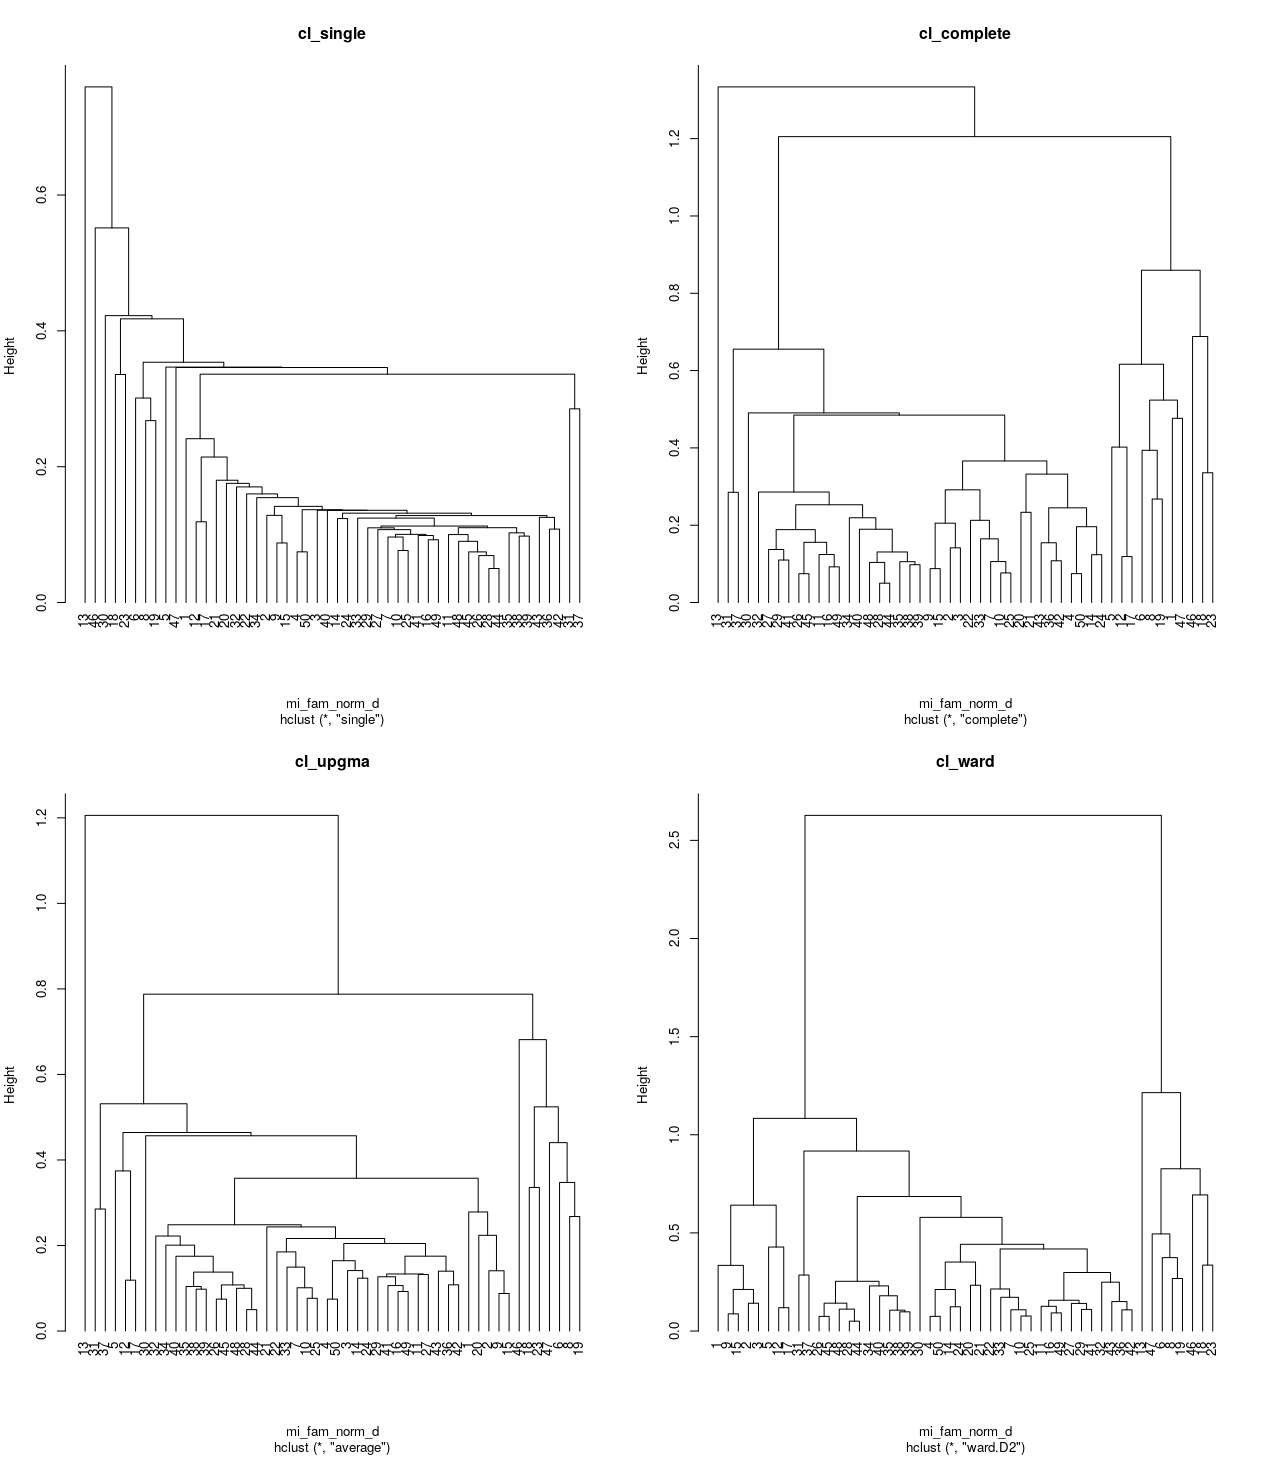
\includegraphics[width=1.00000\textwidth]{enlace_agrpados_metodos.png}
\caption{matriz de comunidad normalizada\label{agrupado}}
\end{figure}

\begin{figure}
\centering
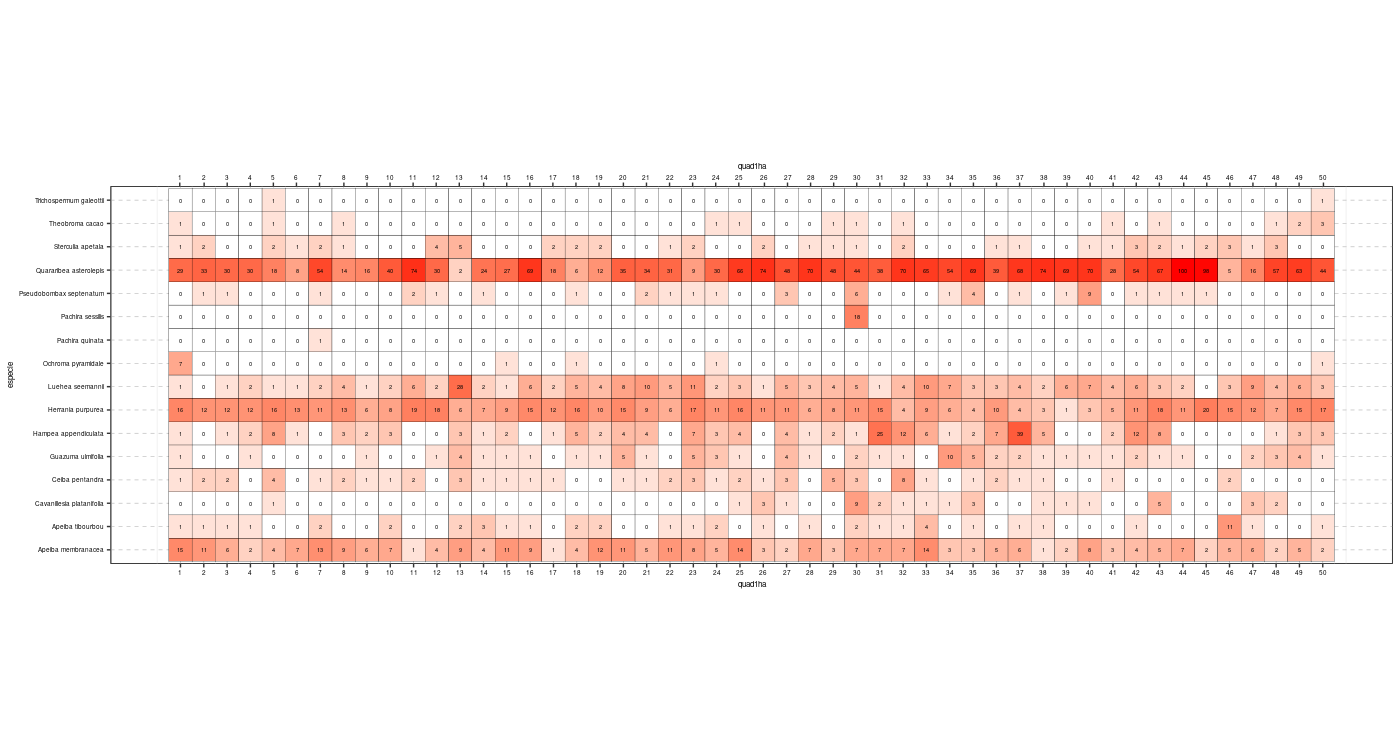
\includegraphics{especies.png}
\caption{Representación de especies por abundancia de
sitio\label{abundancia}}
\end{figure}

\begin{figure}
\centering
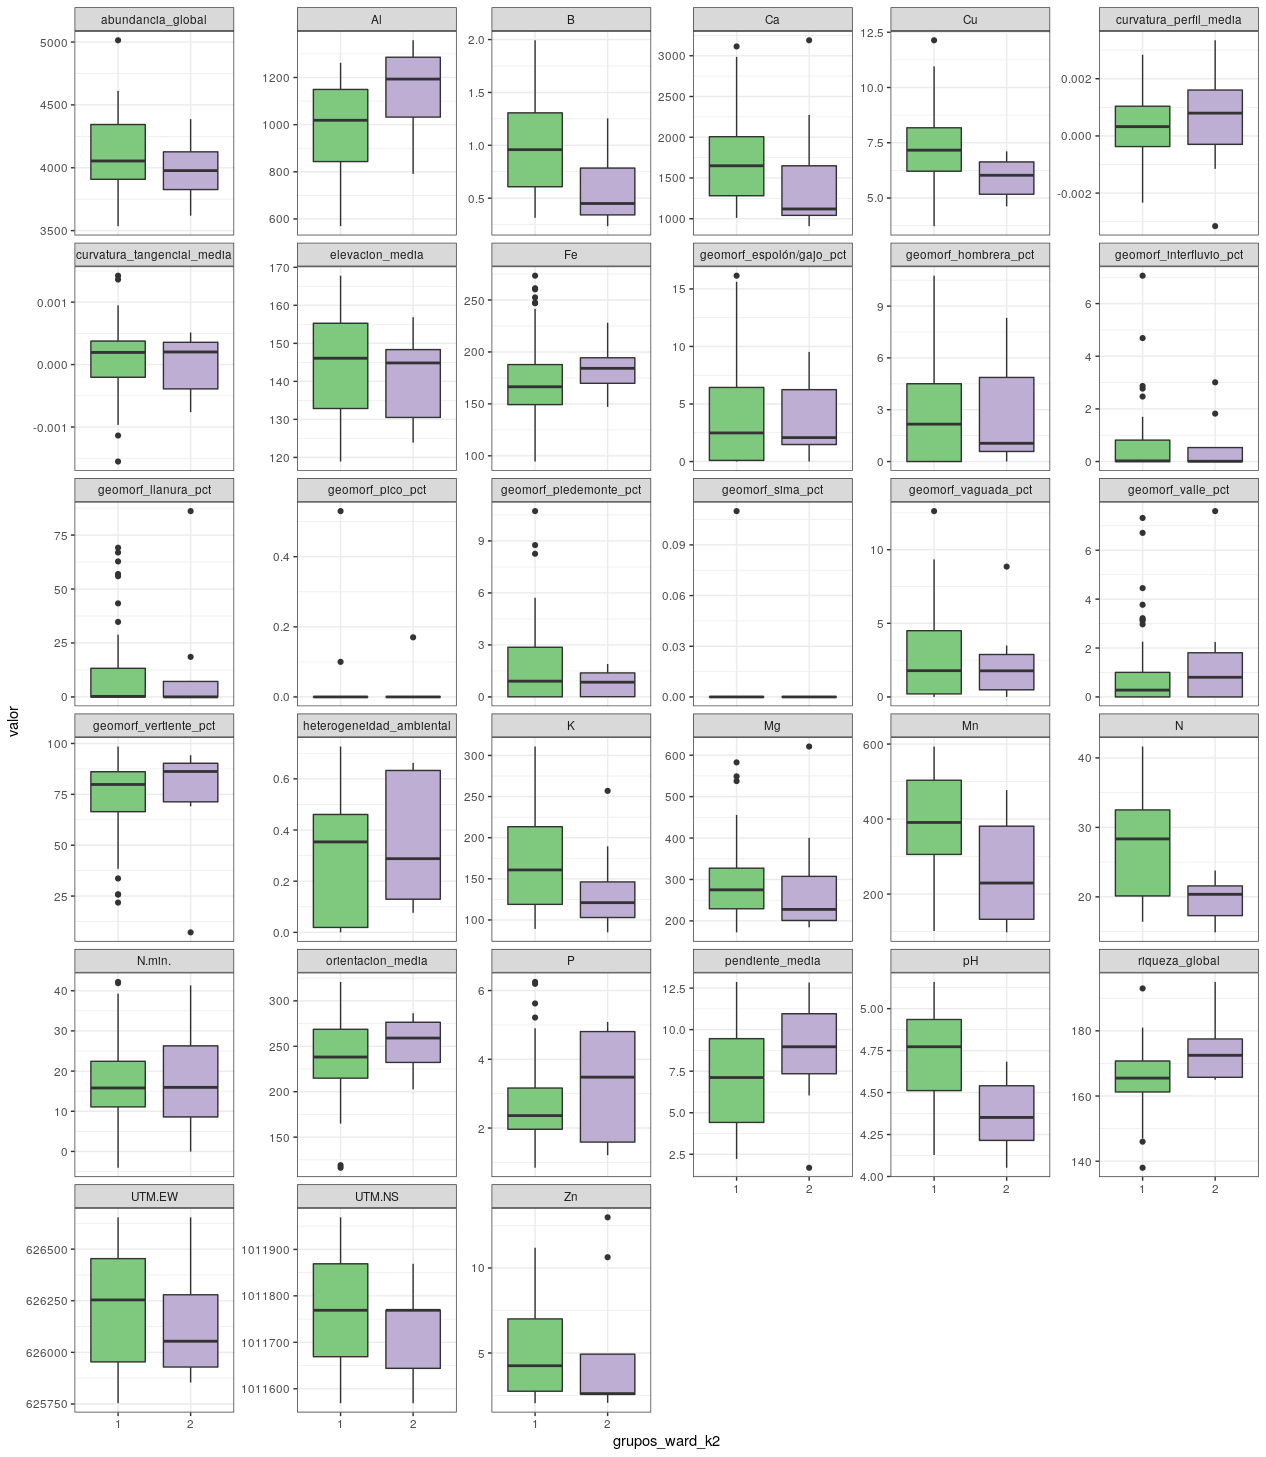
\includegraphics[width=1.10000\textwidth]{Rplot01_diagrama_caja_agrpados.png}
\caption{Representación de especies por abundancia de
sitio\label{homogeneidades}}
\end{figure}

\begin{longtable}[]{@{}lrr@{}}
\caption{Homogeneidad de promedios de variables
ambientales\label{promedio}}\tabularnewline
\toprule
variable & Valor de p, prueba t & Valor de p, prueba
Wilcoxon\tabularnewline
\midrule
\endfirsthead
\toprule
variable & Valor de p, prueba t & Valor de p, prueba
Wilcoxon\tabularnewline
\midrule
\endhead
N & 0.00 & 0.02\tabularnewline
pH & 0.00 & 0.00\tabularnewline
Cu & 0.01 & 0.03\tabularnewline
B & 0.02 & 0.02\tabularnewline
geomorf\_piedemonte\_pct & 0.02 & 0.43\tabularnewline
Mn & 0.04 & 0.03\tabularnewline
riqueza\_global & 0.05 & 0.04\tabularnewline
Al & 0.11 & 0.05\tabularnewline
\bottomrule
\end{longtable}

Al aplicar las diferentes métricas como la equidad de \emph{Shannon}, la
antropía \emph{simpson} y la ratio de \emph{Hill} para conocer la
abundancia y riqueza de especies por cada sitio, se observó una alta
correlación entre cada una a través del método de \emph{Pearson} a
excepción de la ratio de \emph{Hill} donde fue menor. También, en
conformidad con las variables ambientales la abundancia de la familia
fue mayor en presencia del zinc (Zn), nitrogeno (N) y el pH con valores
de 0.45\%, 0.47\% y 0.66\% respectivamente. En tanto, que la riqueza
global predominó en la zona donde el pH fue más idóneo con estimado de
-0.48\% (ver figura\ref{ambiente}). Por otro lado, en los modelos de
abundancia de especies los sitios alpha con mayor y menor riqueza son el
30 y 45 con 13 y 5 especies sucesivamente, los de máxima y mínima
abundancia fue el 6 y 37 con un rango entre 31 y 127. Siendo el lugar
más rico el 30 donde abundan 110 grupos y el más pobre el 45 con 123.
Mientras, que los sitios que contribuyen a la diversidad beta al
implementar el modelo de un único número con la matriz de comunidad con
el método de \emph{Helliger} fueron el 13 con 0.12\% y 46 con 0.82\%. En
tanto, que las especies contribuidoras son la \emph{Quararibea
asterolepis}, \emph{Hampea appendiculata} y \emph{Herrania purpurea} con
0.18\%, 0.14\% y 0.11\%, respectivamente (ver tabla \ref{beta}).

En tanto, que la rarefacción a la abundancia más pequeña encontrada fue
en la zona 45 con 5 y la estimación de individuo por abundancia de grupo
de 3,393. Asimismo, al combinar los grupos y ubicarlo en un solo lugar
por medio del enfoque asintótico, se observó que exceden un total de
3,789 individuos y 14 especie. Dentro de las mismas se encuentran 4
sujeto y 2 clases raras con un estimado de cobertura muestral de 0.67\%
para plantas extrañas, con grado de 16\% de homogéneidad, con un nivel
bajo de 16\% y superior 17.72\%. En Cuanto, a la matriz con el enfoque
no asintótico se registró un espacio con 3,792 individuo y 16 grupos, al
relacionarla con la antropía de \emph{Shannon} se estimó un 4.68\% y con
la equidad de \emph{Simpson} un 2.77\% de diversidad. Por otro lado, al
agrupar la comunidad según el método de Ward se visualizó una cantidad
de 3,393 sujeto, 13 clase, con 13 individuo y 3 grupos inusuales, con
una estimación de 0.92\% de especies.

\begin{longtable}[]{@{}lr@{}}
\caption{Especie contribuidora a la diversidad
beta\label{beta}}\tabularnewline
\toprule
Especie & Valor\tabularnewline
\midrule
\endfirsthead
\toprule
Especie & Valor\tabularnewline
\midrule
\endhead
Apeiba membranacea & 0.08\tabularnewline
Apeiba tibourbou & 0.07\tabularnewline
Hampea appendiculata & 0.14\tabularnewline
Herrania purpurea & 0.11\tabularnewline
Luehea seemannii & 0.09\tabularnewline
Quararibea asterolepis & 0.18\tabularnewline
\bottomrule
\end{longtable}

De acuerdo los datos obtenidos en el análisis de la ecología espacial
por medio de las pruebas de permutación para el \emph{I de Moran} local
se observó una alta correlación de algunas especies en varias zonas
geomorfológicas de la BCI en el orden uno. Donde se estima un 0.42\% en
la llanura, 0.31\% en el espolón, 0.29\% en la vertiente y 0.38\% en la
vaguada, siendo el área del espolón el de más conveniencia. Mientras,
que ante la presencia de ciertos elementos químicos algunas plantas
presentaron una adecuación como fue con el zinc (Zn) con 0.85\%, el
potasio (K) 0.74\%, el calsio (Ca) 0.69 y el pH con 0.72\%. Mientras,
que con el \emph{I de Moran} global aplicado a la abundancia de las
especies de la familia \emph{Malvaceae} las de mayor grado de
autocorrelación fue la \emph{Pachira quinata} con valor de 1\%,
\emph{Pachira sessilis} con 0.71\%, \emph{Guazuma ulmifolia} 0.62\% y la
\emph{Ochroma pyramidale} 0.53\%.

En cuanto, a la matriz de distancia con la prueba Mantel se observó leve
dependencia espacial de algunas especies inducida por variables
ambientales, a medida en que aumenta ésta la autocorrelación es de forma
negativa, siendo el orden 1 y 2 los de más conexión con 4.62\% y -4.95\%
respectivamente. También, mediante el correlograma con una sola variable
los grupos tuvieron una fuerte relación en los siete ordenes primero con
estimaciones entre 0.21\% y 0.72\% en los tres iniciales y desde -0.36\%
a -0.66\% en los cuatro siguientes. Por último, la clase que más abunda
es \emph{Herrania purpurea} con un valor estimado de 0.41\%, seguido por
la \emph{Apeiba membranacea} con 0.36\% (ver figura \ref{distancia} \&
\ref{diversidad}).

\begin{figure}
\centering
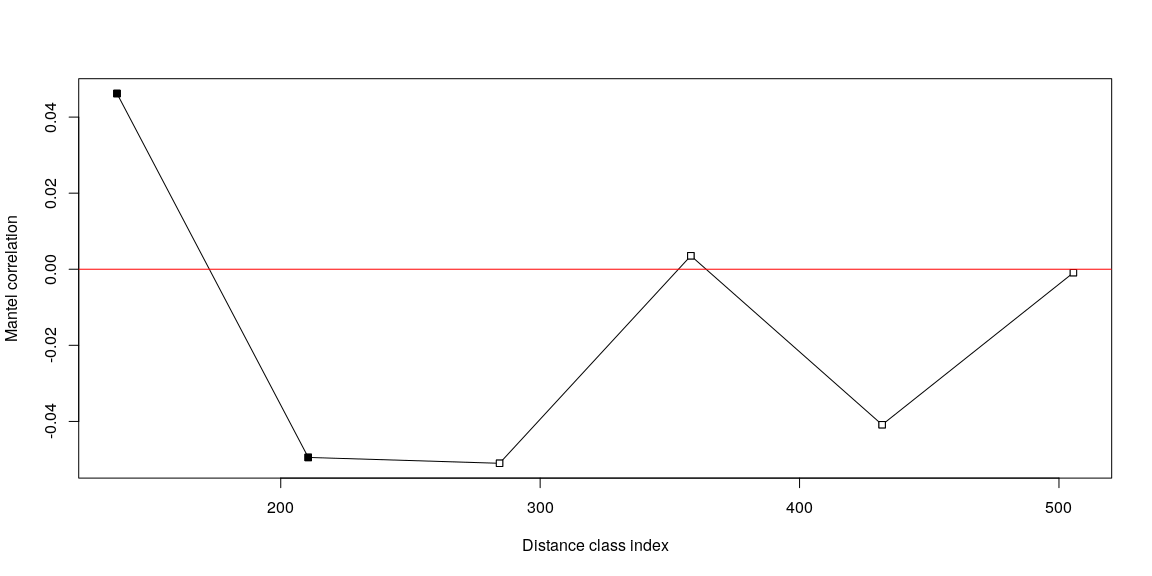
\includegraphics[width=1.00000\textwidth]{ecologia_espacial_files/figure-markdown_github/unnamed-chunk-14-1.png}
\caption{Distancia con prueba Mantel\label{distancia}}
\end{figure}

\begin{figure}
\centering
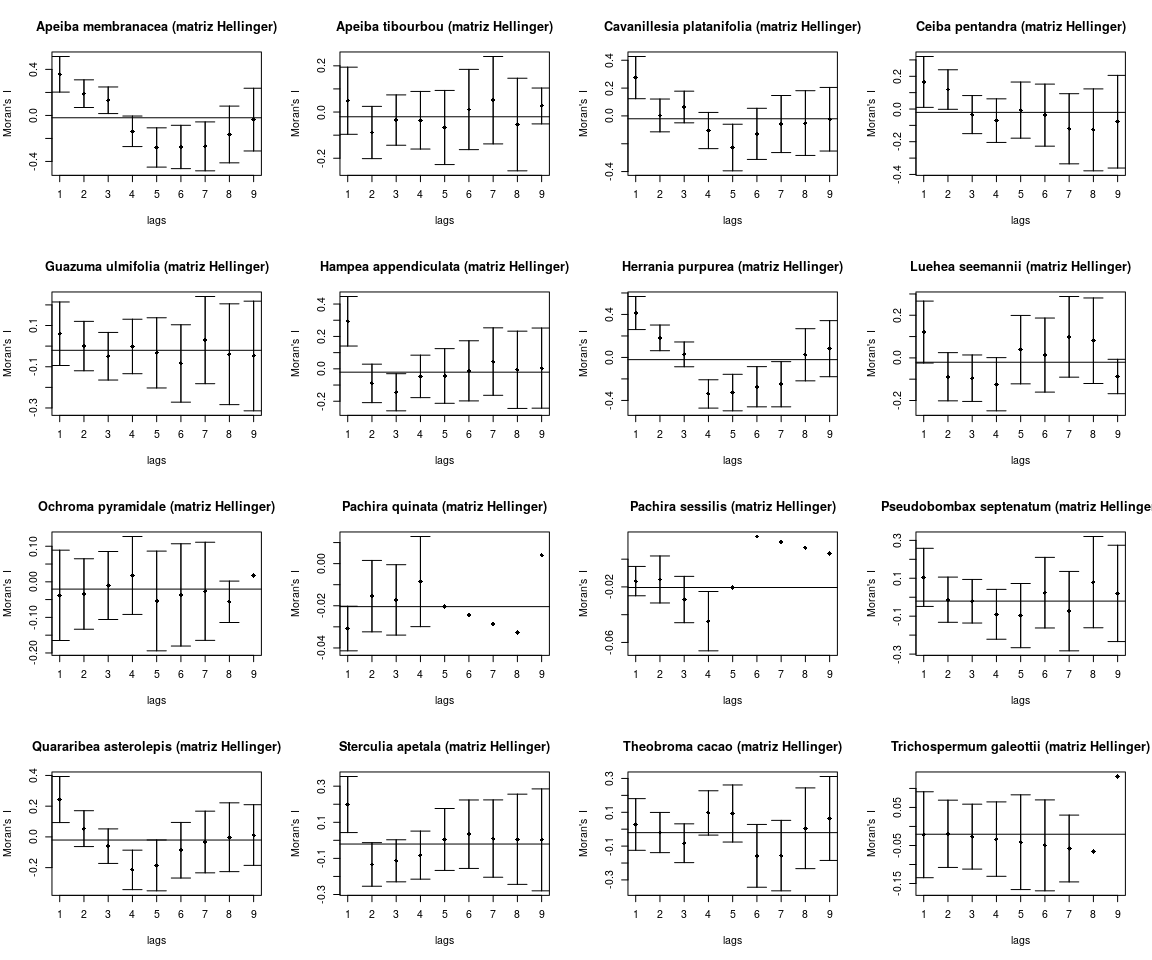
\includegraphics[width=1.10000\textwidth]{ecologia_espacial_files/figure-markdown_github/unnamed-chunk-10-1.png}
\caption{Correlación de las diferentes especies\label{diversidad}}
\end{figure}

\begin{figure}
\centering
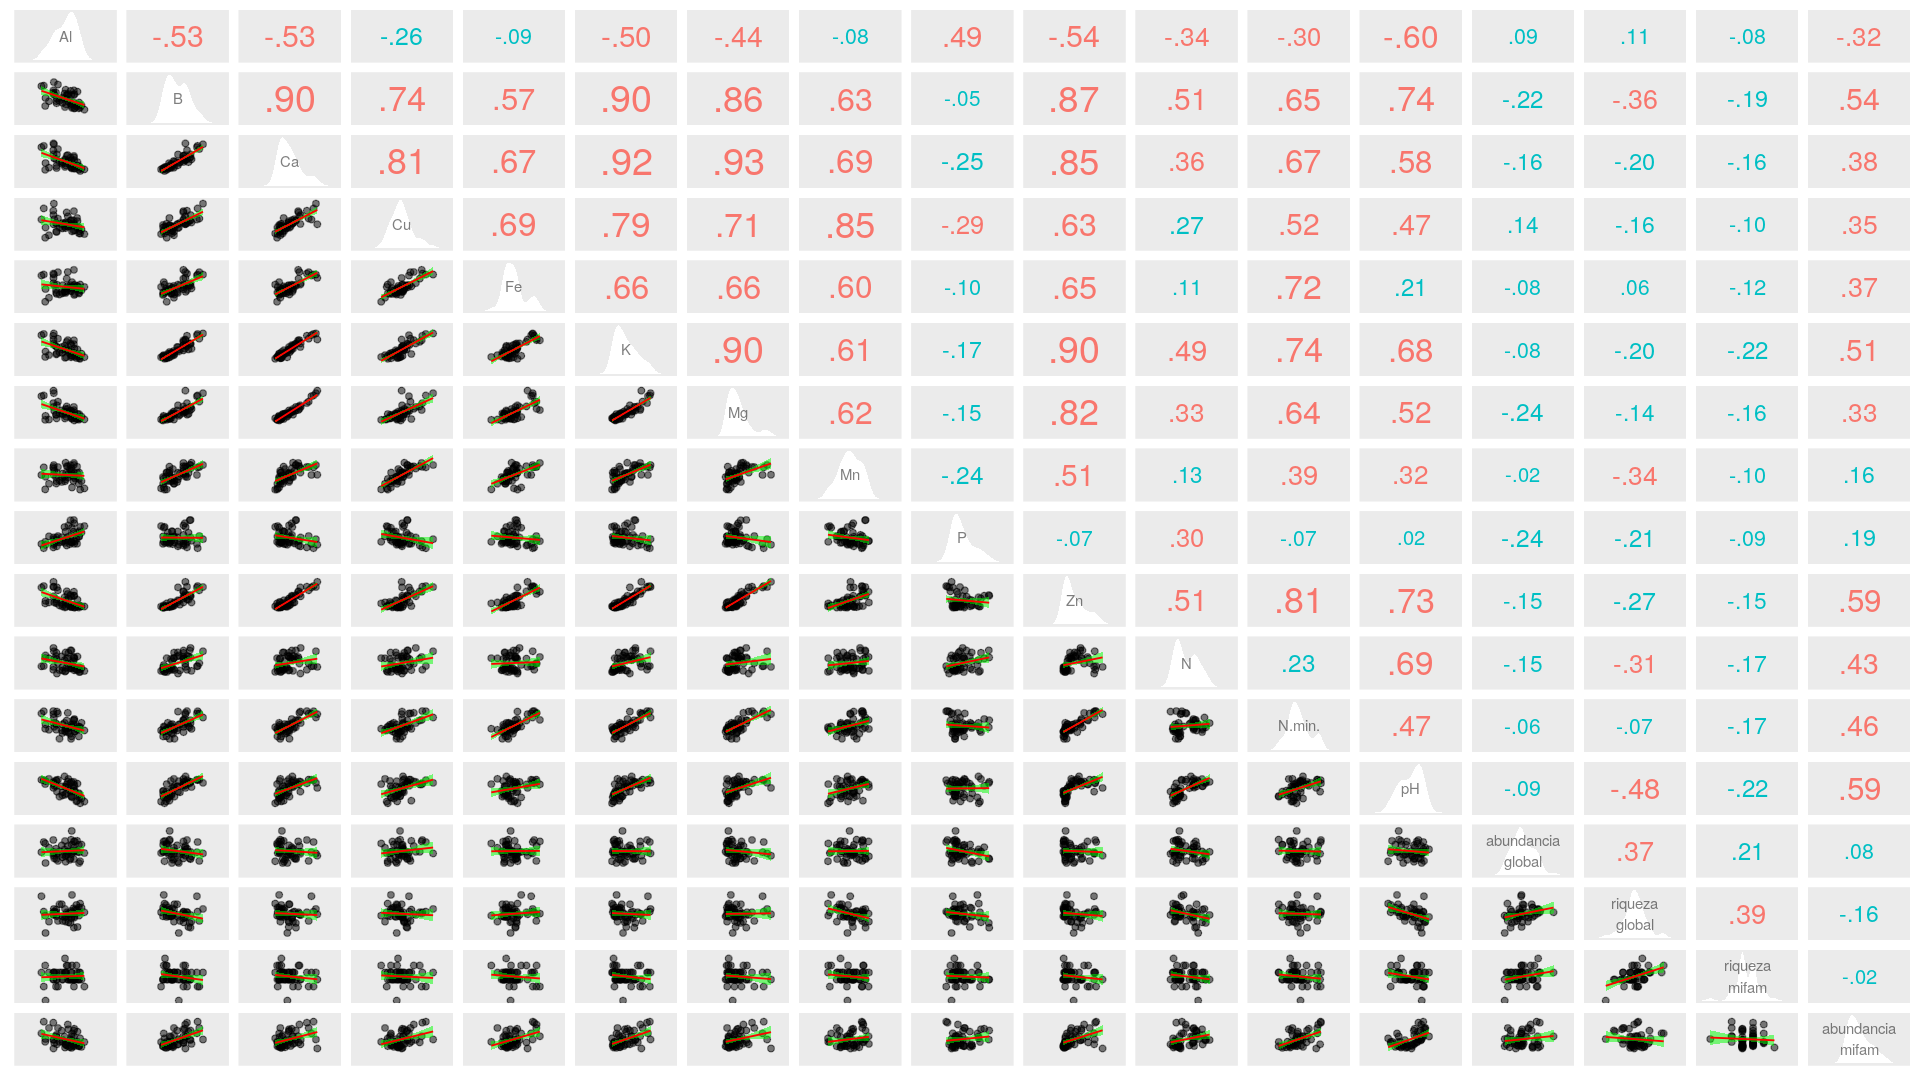
\includegraphics[width=1.10000\textwidth]{matriz_correlacion_suelo_abun_riq_spearman.png}
\caption{Distribución de especies por ambiente\label{ambiente}}
\end{figure}

\section{Discusión}\label{discusiuxf3n}

Los agrupamientos integrados producidos por varias especies en los dos
grupos generados por los diferentes métodos de enlace y donde se
identificó a las plantas \emph{Quararibea asterolepis} y \emph{Sterculia
apetala} como las que más se asocian de manera combinada dentro de la
familia y de manera desigual en el espacio se debe a que algunas sirven
de alimento o de refugio para otros grupos, haciendo que esta se reunan
en un sitio en específico el cual le favorezca en su crecimiento y
desarrollo dispersandola en todo el terreno (Alvarado-Hernández, 2011).

El nivel de representación de la diversidad de especies dado por cada
1,h, fue como resultado de las condisiones climáticas y a la
disponibilidad del agua existente en la zona (Stevenson \& Rodríguez,
2008), razón de que en los sitios más húmedo el nivel de abundancia y
riqueza fue mayor. Además, de la presencia de otras clases que
contribuyeron a la variación espacial de la diversidad entre los lugares
como fue la \emph{Apeiba membranacea}, \emph{Hampea appendiculata}.

En cuanto a la ecología espacial, la formación de patrones discontinuo
por aglomeración en presencia de los elementos químico como el
\emph{zinc} (Zn), el \emph{boro} (B) y el \emph{potasio} (K)
especialmente en la zona de la Vaguada, la llanura, el espolón y la
vertiente indica que ciertas especies de la familia de la
\emph{Malvaceae} son propensas a desarrollarse en sitios con alto
volumen de materia orgánica y gran disponibilidad de agua. Aunque, el
exceso de ciertos elementos pueden afectar la distribución y crecimiento
de ciertas plantas (Clark, 2002), así, como el origen de formación del
suelo los cuales ofrecen ciertas propiedades que definirían el tipo de
colocación (Flores, Suvires, \& Dalmasso, 2015). Esto posiblemente
sucedió en los lugares del piedemonte, el valle, la sima y ante el
conjunto de compuesto como el \emph{fósforo} (P), \emph{cobre} (Cu) y el
\emph{aluminio} (Al) donde la correlación fue menor. También, es posible
que el modelo presentado sea el resuldato por los periodos de sequía que
pudo padecer la parcela en el momento de algunos de la censos, razón de
que este fenómeno en caso de prolongarse podría causar la extinción
local de especies arbóreas (Springer, 1998).

El patrón presentado por las especies de la familia \emph{Malvaceae}
dentro de la parcela permanente de la BCI puede variar al pasar el
tiempo por causa del cambio en el clima. Razón, de que algunos grupos
tienen alta dependencia a desarrollarse en zonas húmeda la cuales pueden
ser afectadas por una temporada de sequía que enfrente ese espacio,
dejando como posibles consecuencias la alteración de las caracteristicas
físicas y la extinción de algunas especies. Posiblemente fue el caso de
la \emph{Apeiba hybrid} quién para los censos de 1981 y 1985 mostró un
área basal de 0.005 y 0.003 respectivamente, mientras que para los
restantes no presentó valor de medición (Hubbell et al., 2021). En tal
sentido, se espera la desaparición de algunas de la clase que componen
dicha familia si el ser humano no diseña estrategias oportunas para
contrarestar las variaciones climáticas y la conservación de las plantas
originarias del bosque.

\section{Agradecimientos}\label{agradecimientos}

Este estudio fue realizado gracias al Dr.~José Ramón Martínez Batlle
maestro de la asignatura de Biogeografía en la Universidad Autónoma de
Santo Domingo (UASD) quién por medio de la escuela de geografía
incentiva al conocimiento a través de la investigación de caracter
científico. También, al Instituto Smithsonian de Instigaciones
Tropicales por suministrar los datos, reslutado de años de observaciones
y puesto a la disposición mediante censos.

\section{Información de soporte}\label{informaciuxf3n-de-soporte}

\begin{Shaded}
\begin{Highlighting}[]
\NormalTok{\textbackslash{}beginsupplement}
\end{Highlighting}
\end{Shaded}

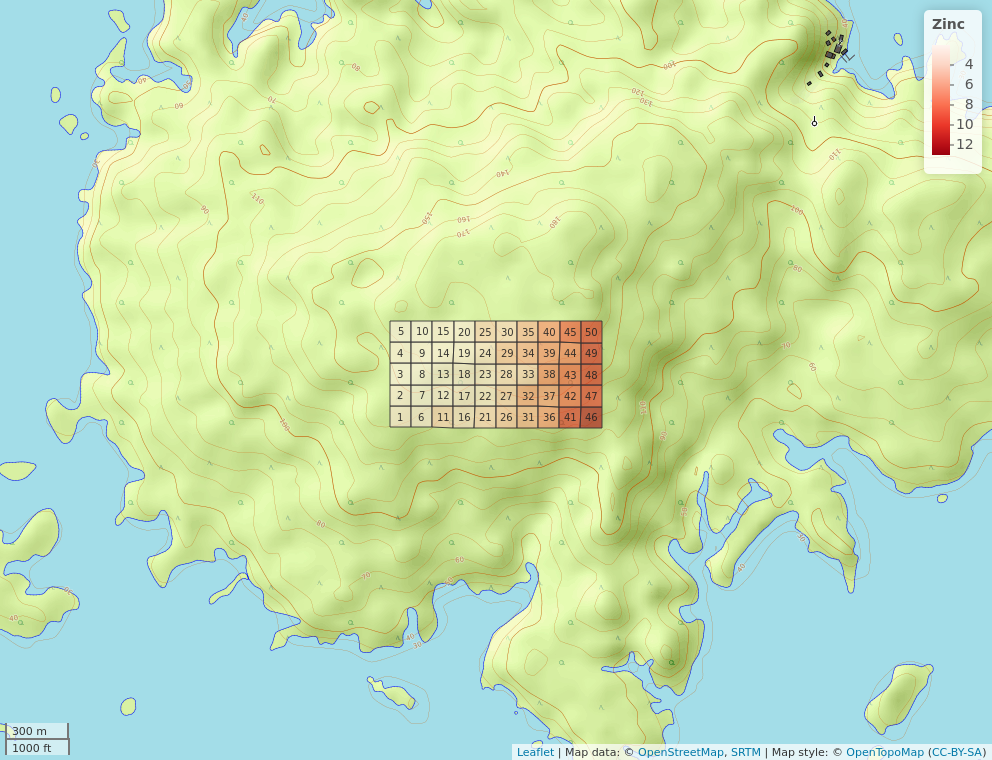
\includegraphics{mapa_zinc.png} \{width=110\%\}

\begin{figure}
\centering
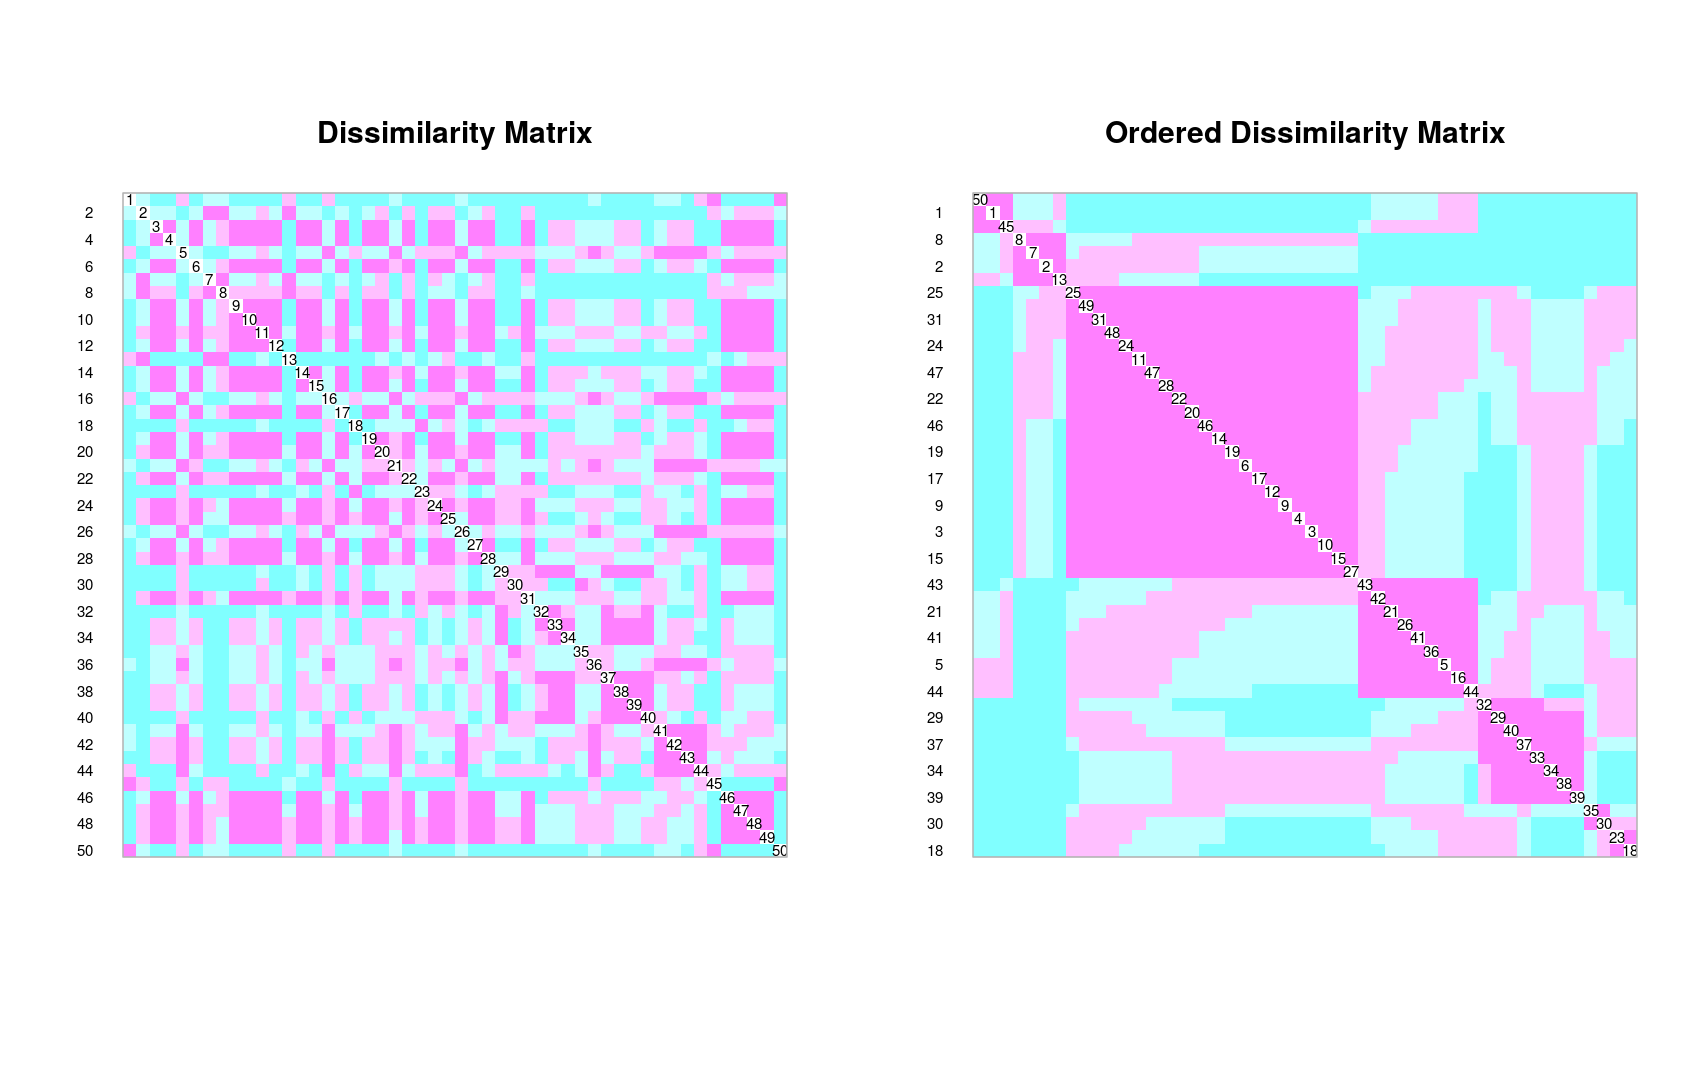
\includegraphics[width=1.10000\textwidth]{mapas_variables_ambientales_numericas.png}
\caption{\label{fig:soporte1} Variables ambientales numéricas}
\end{figure}

\begin{figure}
\centering
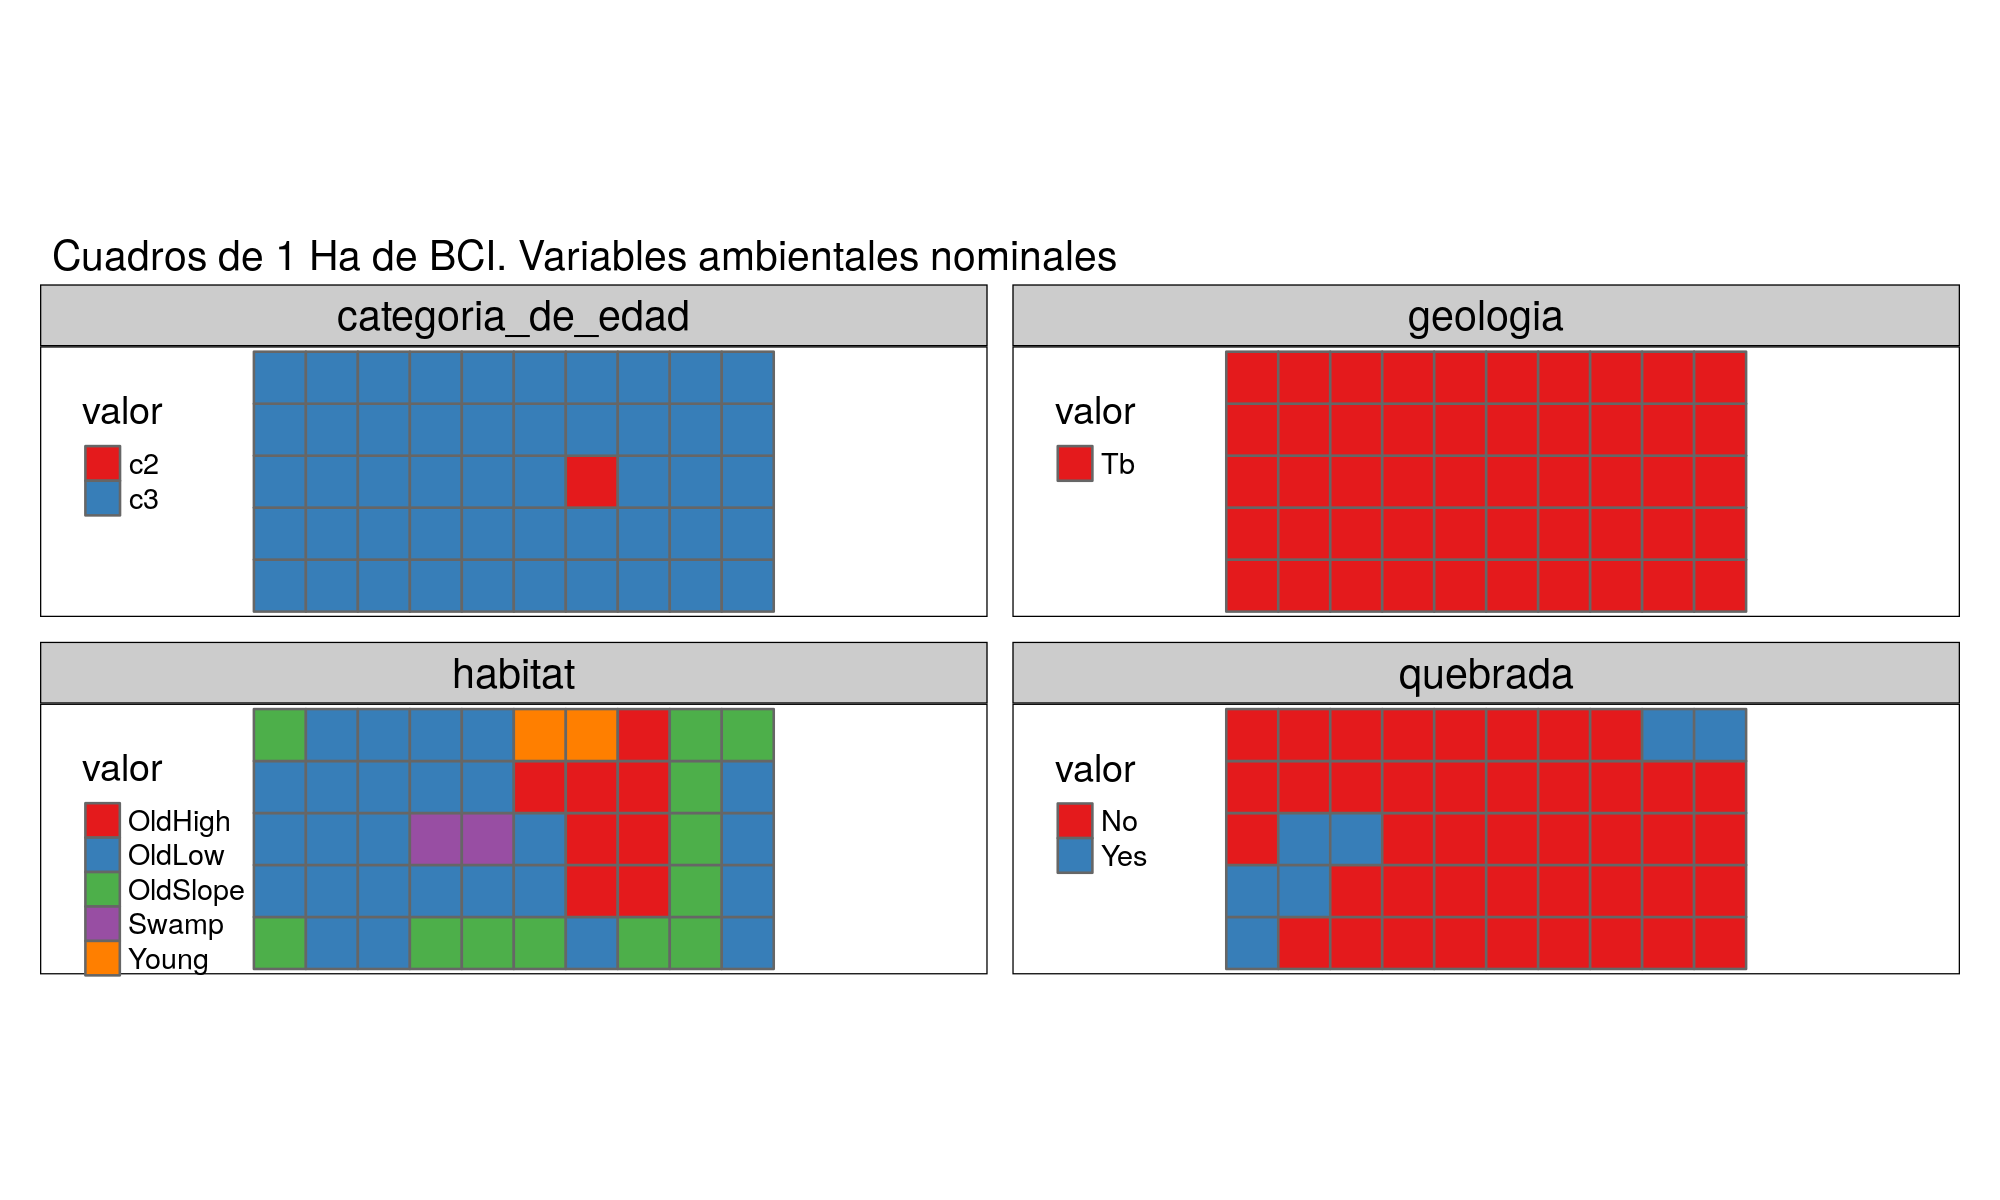
\includegraphics[width=1.10000\textwidth]{mapas_variables_ambientales_nominales_tmap.png}
\caption{\label{fig:soporte1} Variables ambientales nominales}
\end{figure}

\section{\texorpdfstring{\emph{Script}
reproducible}{Script reproducible}}\label{script-reproducible}

\begin{Shaded}
\begin{Highlighting}[]
\KeywordTok{library}\NormalTok{(vegan)}
\KeywordTok{library}\NormalTok{(adespatial)}
\KeywordTok{library}\NormalTok{(broom)}
\KeywordTok{library}\NormalTok{(tidyverse)}
\KeywordTok{library}\NormalTok{(sf)}
\KeywordTok{library}\NormalTok{(gclus)}
\KeywordTok{source}\NormalTok{(}\StringTok{'biodata/funciones.R'}\NormalTok{)}

\KeywordTok{load}\NormalTok{(}\StringTok{'biodata/matriz_ambiental.Rdata'}\NormalTok{)}
\KeywordTok{load}\NormalTok{(}\StringTok{"~/unidad-0-asignacion-99-mi-manuscrito-anavalera29/biodata/Malvaceae.Rdata"}\NormalTok{)}

\NormalTok{mi_fam_t <-}\StringTok{ }\NormalTok{mc_malvc }\OperatorTok\StringTok{ }
\StringTok{  }\KeywordTok{rename_all}\NormalTok{(gsub, }\DataTypeTok{pattern =} \StringTok{' '}\NormalTok{, }\DataTypeTok{replacement =} \StringTok{'}\CharTok{\textbackslash{}n}\StringTok{'}\NormalTok{) }\OperatorTok\StringTok{ }
\StringTok{  }\KeywordTok{t}\NormalTok{()}
\NormalTok{mi_fam_t }\OperatorTok\StringTok{ }\NormalTok{tibble}
 
\NormalTok{mi_fam_t_chi <-}\StringTok{ }\KeywordTok{decostand}\NormalTok{(mi_fam_t, }\StringTok{"chi.square"}\NormalTok{)}
\NormalTok{mi_fam_t_chi }\OperatorTok\StringTok{ }\NormalTok{tibble}
 
\NormalTok{mi_fam_t_chi_d <-}\StringTok{ }\KeywordTok{dist}\NormalTok{(mi_fam_t_chi)}
\NormalTok{mi_fam_t_chi_d }\OperatorTok\StringTok{ }\NormalTok{tidy}
 
\KeywordTok{coldiss}\NormalTok{(mi_fam_t_chi_d, }\DataTypeTok{diag =} \OtherTok{TRUE}\NormalTok{)}

\NormalTok{mi_fam_t_jac <-}\StringTok{ }\KeywordTok{vegdist}\NormalTok{(mi_fam_t, }\StringTok{"jaccard"}\NormalTok{, }\DataTypeTok{binary =} \OtherTok{TRUE}\NormalTok{)}
\NormalTok{mi_fam_t_jac }\OperatorTok\StringTok{ }\NormalTok{tidy}
\KeywordTok{coldiss}\NormalTok{(mi_fam_t_jac, }\DataTypeTok{diag =} \OtherTok{TRUE}\NormalTok{)}

\NormalTok{env_num <-}\StringTok{ }\NormalTok{bci_env_grid }\OperatorTok
\StringTok{  }\NormalTok{dplyr}\OperatorTok{::}\KeywordTok{select_if}\NormalTok{(is.numeric) }\OperatorTok
\StringTok{  }\NormalTok{dplyr}\OperatorTok{::}\KeywordTok{select}\NormalTok{(}\OperatorTok{-}\NormalTok{id, }\OperatorTok{-}\KeywordTok{matches}\NormalTok{(}\StringTok{'^U.*'}\NormalTok{)) }\OperatorTok\StringTok{ }
\StringTok{  }\NormalTok{st_drop_geometry }\OperatorTok\StringTok{ }
\StringTok{  }\KeywordTok{mutate}\NormalTok{(}
    \DataTypeTok{riqueza_mifam =} \KeywordTok{specnumber}\NormalTok{(mc_malvc),}
    \DataTypeTok{abundancia_mifam =} \KeywordTok{rowSums}\NormalTok{(mc_malvc)) }\OperatorTok\StringTok{ }
\StringTok{  }\KeywordTok{rename_all}\NormalTok{(gsub, }\DataTypeTok{pattern =} \StringTok{'_pct$'}\NormalTok{, }\DataTypeTok{replacement =} \StringTok{''}\NormalTok{) }\OperatorTok\StringTok{ }
\StringTok{  }\KeywordTok{rename_all}\NormalTok{(gsub, }\DataTypeTok{pattern =} \StringTok{'_| '}\NormalTok{, }\DataTypeTok{replacement =} \StringTok{'}\CharTok{\textbackslash{}n}\StringTok{'}\NormalTok{)}
\NormalTok{env_num }\OperatorTok\StringTok{ }\NormalTok{tibble}
\end{Highlighting}
\end{Shaded}

\begin{Shaded}
\begin{Highlighting}[]
\CommentTok{#Medición de asociación con el modo Q: matriz de disimilaridad. }
\KeywordTok{library}\NormalTok{(vegan)}
\KeywordTok{library}\NormalTok{(adespatial)}
\KeywordTok{library}\NormalTok{(broom)}
\KeywordTok{library}\NormalTok{(tidyverse)}
\KeywordTok{library}\NormalTok{(sf)}
\KeywordTok{library}\NormalTok{(cluster)}
\KeywordTok{library}\NormalTok{(gclus)}
\KeywordTok{source}\NormalTok{(}\StringTok{'biodata/funciones.R'}\NormalTok{)}

\KeywordTok{load}\NormalTok{(}\StringTok{'biodata/matriz_ambiental.Rdata'}\NormalTok{)}
\KeywordTok{load}\NormalTok{(}\StringTok{"~/unidad-0-asignacion-99-mi-manuscrito-anavalera29/biodata/Malvaceae.Rdata"}\NormalTok{)}

\CommentTok{#' matriz de distancia euclídea, utilizando la transformación *Hellinger*:}
\CommentTok{#' }
\NormalTok{mi_fam_d_hel <-}\StringTok{ }\KeywordTok{dist.ldc}\NormalTok{(mc_malvc, }\StringTok{"hellinger"}\NormalTok{, }\DataTypeTok{silent =}\NormalTok{ T)}
\NormalTok{mi_fam_d_hel }\OperatorTok\StringTok{ }\NormalTok{tidy }\CommentTok{# Para evitar desbordar la consola}
 
\KeywordTok{coldiss}\NormalTok{(mi_fam_d_hel, }\DataTypeTok{diag =}\NormalTok{ T)}

\KeywordTok{coldissgg}\NormalTok{(mi_fam_d_hel, }\DataTypeTok{ordered =}\NormalTok{ T, }\DataTypeTok{nc =} \DecValTok{4}\NormalTok{, }\DataTypeTok{fsz =} \DecValTok{0}\NormalTok{)}

\KeywordTok{coldissgg}\NormalTok{(mi_fam_d_hel, }\DataTypeTok{ordered =}\NormalTok{ T, }\DataTypeTok{nc =} \DecValTok{4}\NormalTok{, }\DataTypeTok{fsz =} \FloatTok{1.5}\NormalTok{)}
 
\KeywordTok{png}\NormalTok{(}
  \DataTypeTok{filename =} \StringTok{'matriz_disimilaridad_hellinger.png'}\NormalTok{,}
  \DataTypeTok{width =} \DecValTok{2400}\NormalTok{, }\DataTypeTok{height =} \DecValTok{1200}\NormalTok{, }\DataTypeTok{pointsize =} \DecValTok{32}
\NormalTok{)}
\KeywordTok{coldiss}\NormalTok{(mi_fam_d_hel, }\DataTypeTok{diag =}\NormalTok{ T)}
\KeywordTok{dev.off}\NormalTok{()}

\OperatorTok{**}\NormalTok{distancia de Jaccard}\OperatorTok{**}\StringTok{ }\NormalTok{(}\OperatorTok{**}\NormalTok{D}\OperatorTok{<}\NormalTok{sub}\OperatorTok{>}\NormalTok{J}\OperatorTok{<}\ErrorTok{/}\NormalTok{sub}\OperatorTok{>}\ErrorTok{**}\NormalTok{) en un único paso usando la función }\StringTok{`}\DataTypeTok{vegdist}\StringTok{`}\NormalTok{.}
\CommentTok{#' }
\NormalTok{mi_fam_jac <-}\StringTok{ }\KeywordTok{vegdist}\NormalTok{(mc_malvc, }\DataTypeTok{method =} \StringTok{'jac'}\NormalTok{, }\DataTypeTok{binary =}\NormalTok{ T)}
\NormalTok{mi_fam_jac }\OperatorTok\StringTok{ }\NormalTok{tidy }\CommentTok{# Mostrando sólo las primeras 10 combinaciones en modo data.frame}

\KeywordTok{coldiss}\NormalTok{(mi_fam_jac, }\DataTypeTok{diag =}\NormalTok{ T)}

\CommentTok{#' }
\NormalTok{(}\DecValTok{1} \OperatorTok{-}\StringTok{ }\NormalTok{mi_fam_jac) }\OperatorTok\StringTok{ }\NormalTok{tidy }\OperatorTok\StringTok{ }\KeywordTok{rename}\NormalTok{(}\DataTypeTok{similaridad=}\NormalTok{distance) }\CommentTok{#Similaridad}

\CommentTok{#' La fórmula de la similaridad de Jaccard es **S<sub>J</sub>=a/(a+b+c)**, donde **a** es el número de especies compartidas (presentes en ambos sitios comparados), **b** el número de especies exclusivas del sitio 2, y **c** el número de especies exclusivas del sitio 1.}
\CommentTok{#' }
\NormalTok{mi_fam_abc <-}\StringTok{ }\KeywordTok{betadiver}\NormalTok{(mc_malvc) }
\NormalTok{mi_fam_abc }\OperatorTok
\StringTok{  }\KeywordTok{map}\NormalTok{(tidy) }\OperatorTok
\StringTok{  }\KeywordTok{map}\NormalTok{(slice, }\DecValTok{1}\NormalTok{) }\OperatorTok
\StringTok{  }\KeywordTok{map_df}\NormalTok{(I, }\DataTypeTok{.id =} \StringTok{'tipo'}\NormalTok{) }\OperatorTok\StringTok{ }
\StringTok{  }\NormalTok{dplyr}\OperatorTok{::}\KeywordTok{select}\NormalTok{(tipo, }\DataTypeTok{n_especies=}\NormalTok{distance)}

\KeywordTok{round}\NormalTok{(}\DecValTok{11}\OperatorTok{/}\DecValTok{12}\OperatorTok{*}\DecValTok{100}\NormalTok{,}\DecValTok{2}\NormalTok{) }\CommentTok{#Porcentaje de especies compartidas = similaridad}

\CommentTok{#' índices de similaridad. Por ejemplo, el Jaccard se calcula así:}
\CommentTok{#' }
\KeywordTok{betadiver}\NormalTok{(mc_malvc, }\DataTypeTok{method =} \StringTok{'j'}\NormalTok{) }\OperatorTok\StringTok{ }\NormalTok{tidy}

\CommentTok{#' Además de la distancia de Jaccard, otra distancia muy utilizada es la de Sorensen o Bray-Curtis. Se calcula fácilmente con la función `vegdist`:}
\CommentTok{#' }
\NormalTok{mi_fam_sor <-}\StringTok{ }\KeywordTok{vegdist}\NormalTok{(mc_malvc, }\DataTypeTok{method =} \StringTok{'bray'}\NormalTok{, }\DataTypeTok{binary =}\NormalTok{ T)}
\NormalTok{mi_fam_sor }\OperatorTok\StringTok{ }\NormalTok{tidy}
\KeywordTok{coldiss}\NormalTok{(mi_fam_sor, }\DataTypeTok{diag =}\NormalTok{ T)}
\CommentTok{#' }
\CommentTok{#' }\AlertTok{###}\CommentTok{ Modo Q para datos cuantitativos, NO de abundancia de especies (variables ambientales)}
 
\NormalTok{env_suelo_punt_z <-}\StringTok{ }\NormalTok{bci_env_grid }\OperatorTok
\StringTok{  }\KeywordTok{st_drop_geometry}\NormalTok{() }\OperatorTok\StringTok{ }
\StringTok{  }\NormalTok{dplyr}\OperatorTok{::}\KeywordTok{select}\NormalTok{(}\KeywordTok{matches}\NormalTok{(}\StringTok{'^[A-T,Z]|^pH$'}\NormalTok{, }\DataTypeTok{ignore.case =}\NormalTok{ F)) }\OperatorTok\StringTok{ }
\StringTok{  }\KeywordTok{scale}\NormalTok{()}
\NormalTok{env_suelo_punt_z_d <-}\StringTok{ }\KeywordTok{dist}\NormalTok{(env_suelo_punt_z)}
\NormalTok{env_suelo_punt_z_d }\OperatorTok\StringTok{ }\NormalTok{tidy}
\KeywordTok{coldiss}\NormalTok{(env_suelo_punt_z_d, }\DataTypeTok{diag =}\NormalTok{ T)}
\CommentTok{#'}
\CommentTok{#' }\AlertTok{###}\CommentTok{ Modo Q para datos cualitativos y cuantitativos (mixtos), NO de abundancia de especies (variables ambientales)}
\CommentTok{#' }

\NormalTok{env_mix <-}\StringTok{ }\NormalTok{bci_env_grid }\OperatorTok
\StringTok{  }\KeywordTok{st_drop_geometry}\NormalTok{() }\OperatorTok
\StringTok{  }\NormalTok{dplyr}\OperatorTok{::}\KeywordTok{select}\NormalTok{(heterogeneidad_ambiental, habitat, quebrada)}
\NormalTok{env_mix_d <-}\StringTok{ }\KeywordTok{daisy}\NormalTok{(}\DataTypeTok{x =}\NormalTok{ env_mix, }\DataTypeTok{metric =} \StringTok{'gower'}\NormalTok{)}
\NormalTok{env_mix_d }\OperatorTok\StringTok{ }\NormalTok{as.dist }\OperatorTok\StringTok{ }\NormalTok{tidy}
\NormalTok{env_mix_d }\OperatorTok\StringTok{ }\KeywordTok{coldiss}\NormalTok{(}\DataTypeTok{diag =}\NormalTok{ T)}
\CommentTok{#'}
\end{Highlighting}
\end{Shaded}

\begin{Shaded}
\begin{Highlighting}[]
\CommentTok{#'Medición de asociación de especie modo R}

\KeywordTok{library}\NormalTok{(vegan)}
\KeywordTok{library}\NormalTok{(adespatial)}
\KeywordTok{library}\NormalTok{(broom)}
\KeywordTok{library}\NormalTok{(tidyverse)}
\KeywordTok{library}\NormalTok{(sf)}
\KeywordTok{library}\NormalTok{(gclus)}
\KeywordTok{source}\NormalTok{(}\StringTok{'biodata/funciones.R'}\NormalTok{)}

\KeywordTok{load}\NormalTok{(}\StringTok{'biodata/matriz_ambiental.Rdata'}\NormalTok{)}
\KeywordTok{load}\NormalTok{(}\StringTok{"~/unidad-0-asignacion-99-mi-manuscrito-anavalera29/biodata/Malvaceae.Rdata"}\NormalTok{)}
\CommentTok{#'}
\CommentTok{#' ## Modo R: matrices de dependencia entre variables (índice de correlación)}
\CommentTok{#' }
\CommentTok{#' }\AlertTok{###}\CommentTok{ Modo R para datos cuantitativos de especies (abundancia)}

\NormalTok{mi_fam_t <-}\StringTok{ }\NormalTok{mc_malvc }\OperatorTok\StringTok{ }
\StringTok{  }\KeywordTok{rename_all}\NormalTok{(gsub, }\DataTypeTok{pattern =} \StringTok{' '}\NormalTok{, }\DataTypeTok{replacement =} \StringTok{'}\CharTok{\textbackslash{}n}\StringTok{'}\NormalTok{) }\OperatorTok\StringTok{ }
\StringTok{  }\KeywordTok{t}\NormalTok{()}
\NormalTok{mi_fam_t }\OperatorTok\StringTok{ }\NormalTok{tibble}
\CommentTok{#' }
\CommentTok{#' Segundo, transformo la matriz transpuesta usando estandarización *Chi*.}
\CommentTok{#' }
\NormalTok{mi_fam_t_chi <-}\StringTok{ }\KeywordTok{decostand}\NormalTok{(mi_fam_t, }\StringTok{"chi.square"}\NormalTok{)}
\NormalTok{mi_fam_t_chi }\OperatorTok\StringTok{ }\NormalTok{tibble}
\CommentTok{#' }
\CommentTok{#' Tercero,  calculo la distancia euclídea.}
\CommentTok{#' }
\NormalTok{mi_fam_t_chi_d <-}\StringTok{ }\KeywordTok{dist}\NormalTok{(mi_fam_t_chi)}
\NormalTok{mi_fam_t_chi_d }\OperatorTok\StringTok{ }\NormalTok{tidy}
\CommentTok{#' }
\CommentTok{#' Finalmente, creo el "mapa de calor".}
\CommentTok{#' }
\KeywordTok{coldiss}\NormalTok{(mi_fam_t_chi_d, }\DataTypeTok{diag =} \OtherTok{TRUE}\NormalTok{)}

\CommentTok{#' }\AlertTok{###}\CommentTok{ Modo R para datos binarios (presencia/ausencia)}
 
\NormalTok{mi_fam_t_jac <-}\StringTok{ }\KeywordTok{vegdist}\NormalTok{(mi_fam_t, }\StringTok{"jaccard"}\NormalTok{, }\DataTypeTok{binary =} \OtherTok{TRUE}\NormalTok{)}
\NormalTok{mi_fam_t_jac }\OperatorTok\StringTok{ }\NormalTok{tidy}
\KeywordTok{coldiss}\NormalTok{(mi_fam_t_jac, }\DataTypeTok{diag =} \OtherTok{TRUE}\NormalTok{)}
\CommentTok{#'}
\CommentTok{#' }\AlertTok{###}\CommentTok{ Modo R para datos cuantitativos, NO de abundancia de especies (variables ambientales)}

\NormalTok{env_num <-}\StringTok{ }\NormalTok{bci_env_grid }\OperatorTok
\StringTok{  }\NormalTok{dplyr}\OperatorTok{::}\KeywordTok{select_if}\NormalTok{(is.numeric) }\OperatorTok
\StringTok{  }\NormalTok{dplyr}\OperatorTok{::}\KeywordTok{select}\NormalTok{(}\OperatorTok{-}\NormalTok{id, }\OperatorTok{-}\KeywordTok{matches}\NormalTok{(}\StringTok{'^U.*'}\NormalTok{)) }\OperatorTok\StringTok{ }
\StringTok{  }\NormalTok{st_drop_geometry }\OperatorTok\StringTok{ }
\StringTok{  }\KeywordTok{mutate}\NormalTok{(}
    \DataTypeTok{riqueza_mifam =} \KeywordTok{specnumber}\NormalTok{(mc_malvc),}
    \DataTypeTok{abundancia_mifam =} \KeywordTok{rowSums}\NormalTok{(mc_malvc)) }\OperatorTok\StringTok{ }
\StringTok{  }\KeywordTok{rename_all}\NormalTok{(gsub, }\DataTypeTok{pattern =} \StringTok{'_pct$'}\NormalTok{, }\DataTypeTok{replacement =} \StringTok{''}\NormalTok{) }\OperatorTok\StringTok{ }
\StringTok{  }\KeywordTok{rename_all}\NormalTok{(gsub, }\DataTypeTok{pattern =} \StringTok{'_| '}\NormalTok{, }\DataTypeTok{replacement =} \StringTok{'}\CharTok{\textbackslash{}n}\StringTok{'}\NormalTok{)}
\NormalTok{env_num }\OperatorTok\StringTok{ }\NormalTok{tibble}
\end{Highlighting}
\end{Shaded}

\begin{Shaded}
\begin{Highlighting}[]
\CommentTok{#'Técnica de ordenación}

\KeywordTok{library}\NormalTok{(vegan)}
\KeywordTok{library}\NormalTok{(tidyverse)}
\KeywordTok{library}\NormalTok{(sf)}
\KeywordTok{library}\NormalTok{(mapview)}
\KeywordTok{source}\NormalTok{(}\StringTok{'biodata/funciones.R'}\NormalTok{)}
\CommentTok{#' }
\CommentTok{#' }\AlertTok{###}\CommentTok{ Cargar datos}
\CommentTok{#' }
\KeywordTok{load}\NormalTok{(}\StringTok{"~/unidad-0-asignacion-99-mi-manuscrito-anavalera29/biodata/Malvaceae.Rdata"}\NormalTok{)}
\KeywordTok{load}\NormalTok{(}\StringTok{'biodata/matriz_ambiental.Rdata'}\NormalTok{)}
\NormalTok{mi_fam <-}\StringTok{ }\NormalTok{mc_malvc}
\NormalTok{(}\KeywordTok{colnames}\NormalTok{(mi_fam) <-}\StringTok{ }\KeywordTok{make.cepnames}\NormalTok{(}\KeywordTok{colnames}\NormalTok{(mi_fam)))}
\NormalTok{(df_equivalencias <-}\StringTok{ }\KeywordTok{data.frame}\NormalTok{(}
  \DataTypeTok{nombre_original =} \KeywordTok{colnames}\NormalTok{(mc_malvc),}
  \KeywordTok{colnames}\NormalTok{(mi_fam)))}
\NormalTok{bci_env_grid }\OperatorTok\StringTok{ }\NormalTok{tibble}
\NormalTok{grupos_upgma_k2 <-}\StringTok{ }\KeywordTok{readRDS}\NormalTok{(}\StringTok{'grupos_upgma_k2.RDS'}\NormalTok{)}
\KeywordTok{table}\NormalTok{(grupos_upgma_k2)}
\NormalTok{grupos_ward_k2 <-}\StringTok{ }\KeywordTok{readRDS}\NormalTok{(}\StringTok{'grupos_ward_k2.RDS'}\NormalTok{)}
\KeywordTok{table}\NormalTok{(grupos_ward_k2)}
\CommentTok{#'Matriz de correlaciones y obtener vectores propios para el PCA.}
\CommentTok{#' }
\NormalTok{env_suelo <-}\StringTok{ }\NormalTok{bci_env_grid }\OperatorTok
\StringTok{  }\NormalTok{st_drop_geometry }\OperatorTok
\StringTok{  }\NormalTok{dplyr}\OperatorTok{::}\KeywordTok{select}\NormalTok{(}\KeywordTok{matches}\NormalTok{(}\StringTok{'^[A-T,Z]|^pH$'}\NormalTok{, }\DataTypeTok{ignore.case =}\NormalTok{ F))}
\NormalTok{env_suelo }\OperatorTok\StringTok{ }\NormalTok{tibble}
\NormalTok{env_suelo_pca <-}\StringTok{ }\KeywordTok{rda}\NormalTok{(env_suelo, }\DataTypeTok{scale =} \OtherTok{TRUE}\NormalTok{)}
\NormalTok{env_suelo_pca}
\KeywordTok{summary}\NormalTok{(env_suelo_pca)}

\CommentTok{#' }
\KeywordTok{screeplot}\NormalTok{(env_suelo_pca, }\DataTypeTok{bstick =} \OtherTok{TRUE}\NormalTok{)}
\CommentTok{#' }
\CommentTok{#' Usando función `cleanplot.pca`}
\CommentTok{#' }
\KeywordTok{par}\NormalTok{(}\DataTypeTok{mfrow =} \KeywordTok{c}\NormalTok{(}\DecValTok{1}\NormalTok{, }\DecValTok{2}\NormalTok{))}
\KeywordTok{cleanplot.pca}\NormalTok{(env_suelo_pca, }\DataTypeTok{scaling =} \DecValTok{1}\NormalTok{, }\DataTypeTok{mar.percent =} \FloatTok{0.08}\NormalTok{, }\DataTypeTok{cex.char1 =} \FloatTok{1.5}\NormalTok{)}
\KeywordTok{cleanplot.pca}\NormalTok{(env_suelo_pca, }\DataTypeTok{scaling =} \DecValTok{2}\NormalTok{, }\DataTypeTok{mar.percent =} \FloatTok{0.04}\NormalTok{, }\DataTypeTok{cex.char1 =} \FloatTok{1.5}\NormalTok{)}
\KeywordTok{par}\NormalTok{(}\DataTypeTok{mfrow =} \KeywordTok{c}\NormalTok{(}\DecValTok{1}\NormalTok{, }\DecValTok{1}\NormalTok{))}
\CommentTok{#' }
\CommentTok{#' Comparar distribución de los sitios en biplots con distribución real en el mapa:}
\CommentTok{#' }
\CommentTok{#' }\AlertTok{###}\CommentTok{ Generar mapa de cuadros sin simbología}
\CommentTok{#' }
\NormalTok{mapa_cuadros <-}\StringTok{ }\KeywordTok{mapView}\NormalTok{(}
\NormalTok{  bci_env_grid,}
  \DataTypeTok{col.regions =} \StringTok{'grey80'}\NormalTok{,}
  \DataTypeTok{alpha.regions =} \FloatTok{0.3}\NormalTok{,}
  \DataTypeTok{map.types =} \StringTok{'OpenTopoMap'}\NormalTok{,}
  \DataTypeTok{legend =}\NormalTok{ F, }\DataTypeTok{zoom =} \DecValTok{14}\NormalTok{,}
  \DataTypeTok{zcol =} \StringTok{'id'}\NormalTok{) }\OperatorTok\StringTok{ }\KeywordTok{addStaticLabels}\NormalTok{() }\OperatorTok
\StringTok{  }\NormalTok{leaflet}\OperatorTok{::}\KeywordTok{setView}\NormalTok{(}
    \DataTypeTok{lng =} \OperatorTok{-}\FloatTok{79.85136}\NormalTok{,}
    \DataTypeTok{lat =} \FloatTok{9.15097}\NormalTok{,}
    \DataTypeTok{zoom =} \DecValTok{15}\NormalTok{)}
\NormalTok{mapa_cuadros}
\CommentTok{#' }
\CommentTok{#' Comparar con resultados de un análisis de agrupamiento del mismo conjunto de datos. Primero agrupo mis sitios basado en la misma matriz ambiental fuente del PCA (`env_suelo`), escalándola.}
\CommentTok{#' }
\NormalTok{(env_agrupamiento <-}\StringTok{ }\KeywordTok{hclust}\NormalTok{(}\KeywordTok{dist}\NormalTok{(}\KeywordTok{scale}\NormalTok{(env_suelo)), }\StringTok{'ward.D'}\NormalTok{))}
\NormalTok{(env_grupos <-}\StringTok{ }\KeywordTok{cutree}\NormalTok{(env_agrupamiento, }\DataTypeTok{k =} \DecValTok{3}\NormalTok{))}
\NormalTok{(mi_cluster <-}\StringTok{ }\KeywordTok{factor}\NormalTok{(env_grupos))}
\NormalTok{(mi_cluster_l <-}\StringTok{ }\KeywordTok{levels}\NormalTok{(mi_cluster))}
\NormalTok{(mi_cluster_l_seq <-}\StringTok{ }\DecValTok{1}\OperatorTok{:}\KeywordTok{length}\NormalTok{(mi_cluster_l))}

\CommentTok{#' }
\NormalTok{(puntuaciones <-}\StringTok{ }\KeywordTok{scores}\NormalTok{(env_suelo_pca, }\DataTypeTok{display =} \StringTok{'wa'}\NormalTok{, }\DataTypeTok{scaling =} \DecValTok{1}\NormalTok{))}
\CommentTok{#'}
\CommentTok{#' Luego creo el gráfico base, coloco los puntos sobre el gráfico usando las puntuaciones, les coloco rótulos y, finalmente, coloco leyenda:}
\CommentTok{#'}
\NormalTok{grafico_base <-}\StringTok{ }\KeywordTok{plot}\NormalTok{(}
\NormalTok{  env_suelo_pca,}
  \DataTypeTok{display =} \StringTok{"wa"}\NormalTok{,}
  \DataTypeTok{scaling =} \DecValTok{1}\NormalTok{,}
  \DataTypeTok{type =} \StringTok{"n"}\NormalTok{,}
  \DataTypeTok{main =} \StringTok{"PCA y grupos"}
\NormalTok{)}
\KeywordTok{abline}\NormalTok{(}\DataTypeTok{v =} \DecValTok{0}\NormalTok{, }\DataTypeTok{lty =} \StringTok{"dotted"}\NormalTok{)}
\KeywordTok{abline}\NormalTok{(}\DataTypeTok{h =} \DecValTok{0}\NormalTok{, }\DataTypeTok{lty =} \StringTok{"dotted"}\NormalTok{)}
\ControlFlowTok{for}\NormalTok{ (i }\ControlFlowTok{in}\NormalTok{ mi_cluster_l_seq) \{}
  \KeywordTok{points}\NormalTok{(puntuaciones[mi_cluster }\OperatorTok{==}\StringTok{ }\NormalTok{i, ],}
         \DataTypeTok{pch =}\NormalTok{ (}\DecValTok{14} \OperatorTok{+}\StringTok{ }\NormalTok{i),}
         \DataTypeTok{cex =} \DecValTok{2}\NormalTok{,}
         \DataTypeTok{col =}\NormalTok{ i }\OperatorTok{+}\StringTok{ }\DecValTok{1}\NormalTok{)}
\NormalTok{\}}
\KeywordTok{text}\NormalTok{(puntuaciones, }\KeywordTok{row.names}\NormalTok{(env_suelo), }\DataTypeTok{cex =} \DecValTok{1}\NormalTok{, }\DataTypeTok{pos =} \DecValTok{3}\NormalTok{)}
\KeywordTok{legend}\NormalTok{(}
  \StringTok{"topright"}\NormalTok{, }\CommentTok{# Otras alternativas: "bottomleft", "bottomright" y "topleft"}
  \KeywordTok{paste}\NormalTok{(}\StringTok{"Grupo"}\NormalTok{, }\KeywordTok{c}\NormalTok{(mi_cluster_l_seq)),}
  \DataTypeTok{pch =} \DecValTok{14} \OperatorTok{+}\StringTok{ }\KeywordTok{c}\NormalTok{(mi_cluster_l_seq),}
  \DataTypeTok{col =} \DecValTok{1} \OperatorTok{+}\StringTok{ }\KeywordTok{c}\NormalTok{(mi_cluster_l_seq),}
  \DataTypeTok{pt.cex =} \DecValTok{2}
\NormalTok{)}

\CommentTok{# (mi_cluster_anterior <- grupos_upgma_k2)}
\NormalTok{(mi_cluster_anterior <-}\StringTok{ }\NormalTok{grupos_ward_k2)}
\NormalTok{(mi_cluster_anterior_l <-}\StringTok{ }\KeywordTok{levels}\NormalTok{(mi_cluster_anterior))}
\NormalTok{(mi_cluster_anterior_l_seq <-}\StringTok{ }\DecValTok{1}\OperatorTok{:}\KeywordTok{length}\NormalTok{(mi_cluster_anterior_l))}
\NormalTok{grafico_base <-}\StringTok{ }\KeywordTok{plot}\NormalTok{(}
\NormalTok{  env_suelo_pca,}
  \DataTypeTok{display =} \StringTok{"wa"}\NormalTok{,}
  \DataTypeTok{scaling =} \DecValTok{1}\NormalTok{,}
  \DataTypeTok{type =} \StringTok{"n"}\NormalTok{,}
  \DataTypeTok{main =} \StringTok{"PCA y grupos"}
\NormalTok{)}
\KeywordTok{abline}\NormalTok{(}\DataTypeTok{v =} \DecValTok{0}\NormalTok{, }\DataTypeTok{lty =} \StringTok{"dotted"}\NormalTok{)}
\KeywordTok{abline}\NormalTok{(}\DataTypeTok{h =} \DecValTok{0}\NormalTok{, }\DataTypeTok{lty =} \StringTok{"dotted"}\NormalTok{)}
\ControlFlowTok{for}\NormalTok{ (i }\ControlFlowTok{in}\NormalTok{ mi_cluster_anterior_l_seq) \{}
  \KeywordTok{points}\NormalTok{(puntuaciones[mi_cluster_anterior }\OperatorTok{==}\StringTok{ }\NormalTok{i, ],}
         \DataTypeTok{pch =}\NormalTok{ (}\DecValTok{14} \OperatorTok{+}\StringTok{ }\NormalTok{i),}
         \DataTypeTok{cex =} \DecValTok{2}\NormalTok{,}
         \DataTypeTok{col =}\NormalTok{ i }\OperatorTok{+}\StringTok{ }\DecValTok{1}\NormalTok{)}
\NormalTok{\}}
\KeywordTok{text}\NormalTok{(puntuaciones, }\KeywordTok{row.names}\NormalTok{(env_suelo), }\DataTypeTok{cex =} \DecValTok{1}\NormalTok{, }\DataTypeTok{pos =} \DecValTok{3}\NormalTok{)}
\KeywordTok{legend}\NormalTok{(}
  \StringTok{"topright"}\NormalTok{, }\CommentTok{# Otras alternativas: "bottomleft", "bottomright" y "topleft"}
  \KeywordTok{paste}\NormalTok{(}\StringTok{"Grupo"}\NormalTok{, }\KeywordTok{c}\NormalTok{(mi_cluster_anterior_l_seq)),}
  \DataTypeTok{pch =} \DecValTok{14} \OperatorTok{+}\StringTok{ }\KeywordTok{c}\NormalTok{(mi_cluster_anterior_l_seq),}
  \DataTypeTok{col =} \DecValTok{1} \OperatorTok{+}\StringTok{ }\KeywordTok{c}\NormalTok{(mi_cluster_anterior_l_seq),}
  \DataTypeTok{pt.cex =} \DecValTok{2}
\NormalTok{)}
 
\CommentTok{#' #### PCA aplicado a datos de comunidad transformados}
\CommentTok{#' }
\NormalTok{mi_fam_hel <-}\StringTok{ }\KeywordTok{decostand}\NormalTok{(mi_fam, }\DataTypeTok{method =} \StringTok{'hellinger'}\NormalTok{)}
\NormalTok{mi_fam_hel }\OperatorTok\StringTok{ }\NormalTok{tibble}
\NormalTok{mi_fam_hel_pca <-}\StringTok{ }\KeywordTok{rda}\NormalTok{(mi_fam_hel)}
\KeywordTok{summary}\NormalTok{(mi_fam_hel_pca)}
\KeywordTok{screeplot}\NormalTok{(}
\NormalTok{  mi_fam_hel_pca,}
  \DataTypeTok{bstick =} \OtherTok{TRUE}\NormalTok{,}
  \DataTypeTok{npcs =} \KeywordTok{length}\NormalTok{(mi_fam_hel_pca}\OperatorTok{$}\NormalTok{CA}\OperatorTok{$}\NormalTok{eig)}
\NormalTok{)}
\NormalTok{mi_fam_hel_pca_sc1 <-}\StringTok{ }\KeywordTok{scores}\NormalTok{(mi_fam_hel_pca,}
                             \DataTypeTok{display =} \StringTok{"species"}\NormalTok{, }\DataTypeTok{scaling =} \DecValTok{1}\NormalTok{)}
\NormalTok{mi_fam_hel_pca_sc2 <-}\StringTok{ }\KeywordTok{scores}\NormalTok{(mi_fam_hel_pca,}
                             \DataTypeTok{display =} \StringTok{"species"}\NormalTok{, }\DataTypeTok{scaling =} \DecValTok{2}\NormalTok{)}
\KeywordTok{par}\NormalTok{(}\DataTypeTok{mfrow =} \KeywordTok{c}\NormalTok{(}\DecValTok{1}\NormalTok{, }\DecValTok{2}\NormalTok{))}
\KeywordTok{cleanplot.pca}\NormalTok{(mi_fam_hel_pca, }\DataTypeTok{scaling =} \DecValTok{1}\NormalTok{, }\DataTypeTok{mar.percent =} \FloatTok{0.06}\NormalTok{, }\DataTypeTok{cex.char1 =} \FloatTok{0.7}\NormalTok{)}
\KeywordTok{cleanplot.pca}\NormalTok{(mi_fam_hel_pca, }\DataTypeTok{scaling =} \DecValTok{2}\NormalTok{, }\DataTypeTok{mar.percent =} \FloatTok{0.06}\NormalTok{, }\DataTypeTok{cex.char1 =} \FloatTok{0.7}\NormalTok{)}
\KeywordTok{par}\NormalTok{(}\DataTypeTok{mfrow =} \KeywordTok{c}\NormalTok{(}\DecValTok{1}\NormalTok{, }\DecValTok{1}\NormalTok{))}

\KeywordTok{biplot}\NormalTok{(}
\NormalTok{  mi_fam_hel_pca,}
  \DataTypeTok{main =} \StringTok{"PCA, escalamiento 2, ajuste a variables ambientales"}\NormalTok{)}
\NormalTok{(mi_fam_hel_pca_envfit <-}\StringTok{ }\KeywordTok{envfit}\NormalTok{(mi_fam_hel_pca, env_suelo, }\DataTypeTok{scaling =} \DecValTok{2}\NormalTok{))}
\KeywordTok{plot}\NormalTok{(mi_fam_hel_pca_envfit, }\DataTypeTok{p.max =} \FloatTok{0.05}\NormalTok{ , }\DataTypeTok{col =} \DecValTok{3}\NormalTok{)}

\NormalTok{env_num <-}\StringTok{ }\NormalTok{bci_env_grid }\OperatorTok
\StringTok{  }\KeywordTok{select_if}\NormalTok{(is.numeric) }\OperatorTok
\StringTok{  }\KeywordTok{select}\NormalTok{(}\OperatorTok{-}\NormalTok{id) }\OperatorTok
\StringTok{  }\NormalTok{st_drop_geometry}
\NormalTok{(mi_fam_hel_pca_envfit_num <-}\StringTok{ }\KeywordTok{envfit}\NormalTok{(mi_fam_hel_pca, env_num, }\DataTypeTok{scaling =} \DecValTok{2}\NormalTok{))}
\KeywordTok{biplot}\NormalTok{(}
\NormalTok{  mi_fam_hel_pca,}
  \DataTypeTok{main =} \StringTok{"PCA, escalamiento 2, ajuste a variables ambientales"}\NormalTok{)}
\KeywordTok{plot}\NormalTok{(mi_fam_hel_pca_envfit_num, }\DataTypeTok{p.max =} \FloatTok{0.05}\NormalTok{ , }\DataTypeTok{col =} \DecValTok{3}\NormalTok{)}
\KeywordTok{biplot}\NormalTok{(}
\NormalTok{  mi_fam_hel_pca,}
  \DataTypeTok{main =} \StringTok{"PCA, escalamiento 2, ajuste a variables ambientales"}\NormalTok{)}
\KeywordTok{plot}\NormalTok{(mi_fam_hel_pca_envfit_num, }\DataTypeTok{p.max =} \FloatTok{0.1}\NormalTok{ , }\DataTypeTok{col =} \DecValTok{3}\NormalTok{)}
 
\CommentTok{#' }\AlertTok{###}\CommentTok{ Análisis de correspondencia (CA)}
\CommentTok{#' }
\NormalTok{mi_fam_ca <-}\StringTok{ }\KeywordTok{cca}\NormalTok{(mi_fam)}
\KeywordTok{summary}\NormalTok{(mi_fam_ca)}
\KeywordTok{summary}\NormalTok{(mi_fam_ca, }\DataTypeTok{scaling =} \DecValTok{1}\NormalTok{)}
\CommentTok{#'}
\CommentTok{#' Screeplot}
\CommentTok{#' }
\KeywordTok{screeplot}\NormalTok{(mi_fam_ca, }\DataTypeTok{bstick =} \OtherTok{TRUE}\NormalTok{, }\DataTypeTok{npcs =} \KeywordTok{length}\NormalTok{(mi_fam_ca}\OperatorTok{$}\NormalTok{CA}\OperatorTok{$}\NormalTok{eig))}
\CommentTok{#'}
\CommentTok{#' Biplots}
\CommentTok{#' }
\KeywordTok{par}\NormalTok{(}\DataTypeTok{mfrow =} \KeywordTok{c}\NormalTok{(}\DecValTok{1}\NormalTok{, }\DecValTok{2}\NormalTok{))}
\KeywordTok{plot}\NormalTok{(mi_fam_ca,}
     \DataTypeTok{scaling =} \DecValTok{1}\NormalTok{,}
     \DataTypeTok{main =} \StringTok{"Análisis de correspondencia, escalamiento 1"}
\NormalTok{)}
\KeywordTok{plot}\NormalTok{(mi_fam_ca,}
     \DataTypeTok{scaling =} \DecValTok{2}\NormalTok{, }\CommentTok{# Por defecto scaling=2, lo escribo sólo para fines didáticos}
     \DataTypeTok{main =} \StringTok{"Análisis de correspondencia, escalamiento 2"}\NormalTok{)}
\KeywordTok{par}\NormalTok{(}\DataTypeTok{mfrow =} \KeywordTok{c}\NormalTok{(}\DecValTok{1}\NormalTok{, }\DecValTok{1}\NormalTok{))}
\CommentTok{#' }
\CommentTok{#' Excluyendo especie *Thevetia ahouai*, abreviada como *Thevahou*.}
\CommentTok{#' }
\NormalTok{mi_fam_ca <-}\StringTok{ }\KeywordTok{cca}\NormalTok{(mi_fam[, }\OperatorTok{-}\KeywordTok{grep}\NormalTok{(}\StringTok{'Thevahou'}\NormalTok{, }\KeywordTok{colnames}\NormalTok{(mi_fam))])}
\KeywordTok{summary}\NormalTok{(mi_fam_ca)}
\KeywordTok{summary}\NormalTok{(mi_fam_ca, }\DataTypeTok{scaling =} \DecValTok{1}\NormalTok{)}
\KeywordTok{screeplot}\NormalTok{(mi_fam_ca, }\DataTypeTok{bstick =} \OtherTok{TRUE}\NormalTok{, }\DataTypeTok{npcs =} \KeywordTok{length}\NormalTok{(mi_fam_ca}\OperatorTok{$}\NormalTok{CA}\OperatorTok{$}\NormalTok{eig))}
\KeywordTok{par}\NormalTok{(}\DataTypeTok{mfrow =} \KeywordTok{c}\NormalTok{(}\DecValTok{1}\NormalTok{, }\DecValTok{2}\NormalTok{))}
\KeywordTok{plot}\NormalTok{(mi_fam_ca,}
     \DataTypeTok{scaling =} \DecValTok{1}\NormalTok{,}
     \DataTypeTok{main =} \StringTok{"CA, escalamiento 1, sin Thevetia ahouai"}
\NormalTok{)}
\KeywordTok{plot}\NormalTok{(mi_fam_ca,}
     \DataTypeTok{scaling =} \DecValTok{2}\NormalTok{,}
     \DataTypeTok{main =} \StringTok{"CA, escalamiento 2, sin Thevetia ahouai"}\NormalTok{)}
\KeywordTok{par}\NormalTok{(}\DataTypeTok{mfrow =} \KeywordTok{c}\NormalTok{(}\DecValTok{1}\NormalTok{, }\DecValTok{1}\NormalTok{))}
\CommentTok{#' }
\CommentTok{#' Análisis de coordenadas principales (PCoA)}

\NormalTok{mi_fam_d_bray <-}\StringTok{ }\KeywordTok{vegdist}\NormalTok{(mi_fam, }\DataTypeTok{method =} \StringTok{'bray'}\NormalTok{) }\CommentTok{# En realidad, 'bray' es la opción por defecto}
\NormalTok{mi_fam_d_bray_pcoa <-}\StringTok{ }\KeywordTok{cmdscale}\NormalTok{(}
\NormalTok{  mi_fam_d_bray,}
  \DataTypeTok{k =}\NormalTok{ (}\KeywordTok{nrow}\NormalTok{(mi_fam) }\OperatorTok{-}\StringTok{ }\DecValTok{1}\NormalTok{),}
  \DataTypeTok{add =}\NormalTok{ T,}
  \DataTypeTok{eig =} \OtherTok{TRUE}\NormalTok{)}
\KeywordTok{round}\NormalTok{(mi_fam_d_bray_pcoa}\OperatorTok{$}\NormalTok{eig, }\DecValTok{2}\NormalTok{)}
\KeywordTok{round}\NormalTok{(}\KeywordTok{sum}\NormalTok{(mi_fam_d_bray_pcoa}\OperatorTok{$}\NormalTok{eig[mi_fam_d_bray_pcoa}\OperatorTok{$}\NormalTok{eig}\OperatorTok{<}\DecValTok{0}\NormalTok{]),}\DecValTok{2}\NormalTok{)}
\KeywordTok{round}\NormalTok{(}\KeywordTok{sum}\NormalTok{(mi_fam_d_bray_pcoa}\OperatorTok{$}\NormalTok{eig[mi_fam_d_bray_pcoa}\OperatorTok{$}\NormalTok{eig}\OperatorTok{>=}\DecValTok{0}\NormalTok{]),}\DecValTok{2}\NormalTok{)}
\KeywordTok{ordiplot}\NormalTok{(}\KeywordTok{scores}\NormalTok{(mi_fam_d_bray_pcoa, }\DataTypeTok{choices =} \KeywordTok{c}\NormalTok{(}\DecValTok{1}\NormalTok{, }\DecValTok{2}\NormalTok{)),}
         \DataTypeTok{type =} \StringTok{"t"}\NormalTok{,}
         \DataTypeTok{main =} \StringTok{"PCoA con promedios ponderados de especies"}\NormalTok{)}
\KeywordTok{abline}\NormalTok{(}\DataTypeTok{h =} \DecValTok{0}\NormalTok{, }\DataTypeTok{lty =} \DecValTok{3}\NormalTok{)}
\KeywordTok{abline}\NormalTok{(}\DataTypeTok{v =} \DecValTok{0}\NormalTok{, }\DataTypeTok{lty =} \DecValTok{3}\NormalTok{)}
\NormalTok{mi_fam_d_bray_pcoa_wa <-}\StringTok{ }\KeywordTok{wascores}\NormalTok{(mi_fam_d_bray_pcoa}\OperatorTok{$}\NormalTok{points[, }\DecValTok{1}\OperatorTok{:}\DecValTok{2}\NormalTok{], mi_fam)}
\KeywordTok{text}\NormalTok{(}
\NormalTok{  mi_fam_d_bray_pcoa_wa,}
  \KeywordTok{rownames}\NormalTok{(mi_fam_d_bray_pcoa_wa),}
  \DataTypeTok{cex =} \FloatTok{0.7}\NormalTok{, }\DataTypeTok{col =} \StringTok{"red"}\NormalTok{)}
\NormalTok{(mi_fam_d_bray_pcoa_env <-}\StringTok{ }\KeywordTok{envfit}\NormalTok{(mi_fam_d_bray_pcoa, env_num))}
\KeywordTok{plot}\NormalTok{(mi_fam_d_bray_pcoa_env, }\DataTypeTok{p.max =} \FloatTok{0.05}\NormalTok{, }\DataTypeTok{col =} \DecValTok{3}\NormalTok{)}
\end{Highlighting}
\end{Shaded}

\begin{Shaded}
\begin{Highlighting}[]
\CommentTok{#'Técnica de ordenación 2}

\KeywordTok{library}\NormalTok{(vegan)}
\KeywordTok{library}\NormalTok{(tidyverse)}
\KeywordTok{library}\NormalTok{(sf)}
\KeywordTok{source}\NormalTok{(}\StringTok{'biodata/funciones.R'}\NormalTok{)}
\CommentTok{#' }
\CommentTok{#' }\AlertTok{###}\CommentTok{ Cargar datos}
\CommentTok{#' }
\KeywordTok{load}\NormalTok{(}\StringTok{"~/unidad-0-asignacion-99-mi-manuscrito-anavalera29/biodata/Malvaceae.Rdata"}\NormalTok{)}
\KeywordTok{load}\NormalTok{(}\StringTok{'biodata/matriz_ambiental.Rdata'}\NormalTok{)}
\NormalTok{mi_fam <-}\StringTok{ }\NormalTok{mc_malvc}
\NormalTok{(}\KeywordTok{colnames}\NormalTok{(mi_fam) <-}\StringTok{ }\KeywordTok{make.cepnames}\NormalTok{(}\KeywordTok{colnames}\NormalTok{(mi_fam)))}
\NormalTok{(df_equivalencias <-}\StringTok{ }\KeywordTok{data.frame}\NormalTok{(}
  \DataTypeTok{nombre_original =} \KeywordTok{colnames}\NormalTok{(mc_malvc),}
  \KeywordTok{colnames}\NormalTok{(mi_fam)))}
\NormalTok{bci_env_grid }\OperatorTok\StringTok{ }\NormalTok{tibble}
\CommentTok{#' }
\CommentTok{#' ## Ordenación restringida}

\CommentTok{#' }\AlertTok{###}\CommentTok{ Análisis de redundancia (RDA)}

\CommentTok{#'Matriz ambiental de variables suelo:}
\CommentTok{#' }
\NormalTok{mi_fam_hel <-}\StringTok{ }\KeywordTok{decostand}\NormalTok{(mi_fam, }\DataTypeTok{method =} \StringTok{'hellinger'}\NormalTok{)}
\NormalTok{mi_fam_hel }\OperatorTok\StringTok{ }\NormalTok{tibble}
\NormalTok{env_suelo <-}\StringTok{ }\NormalTok{bci_env_grid }\OperatorTok
\StringTok{  }\NormalTok{st_drop_geometry }\OperatorTok
\StringTok{  }\NormalTok{dplyr}\OperatorTok{::}\KeywordTok{select}\NormalTok{(}\KeywordTok{matches}\NormalTok{(}\StringTok{'^[A-T,Z]|^pH$'}\NormalTok{, }\DataTypeTok{ignore.case =}\NormalTok{ F))}
\NormalTok{env_suelo }\OperatorTok\StringTok{ }\NormalTok{tibble}
\NormalTok{mi_fam_hel_rda_suelo <-}\StringTok{ }\KeywordTok{rda}\NormalTok{(mi_fam_hel }\OperatorTok{~}\StringTok{ }\NormalTok{., env_suelo)}
\KeywordTok{summary}\NormalTok{(mi_fam_hel_rda_suelo)}

\KeywordTok{RsquareAdj}\NormalTok{(mi_fam_hel_rda_suelo)}\OperatorTok{$}\NormalTok{adj.r.squared}

\KeywordTok{vif.cca}\NormalTok{(mi_fam_hel_rda_suelo)}
 
\CommentTok{#'Representación del modelo se realiza en un *triplot*, que es un gráfico enriquecido, puesto que contiene tres elementos: sitios, variables de respuesta (especies) y variables explicativas (variables ambientales). Para los sitios se usan las puntuaciones restringidas de sitio.}
\CommentTok{#' }
\CommentTok{#' Escalamiento 1:}
\CommentTok{#' }
\KeywordTok{plot}\NormalTok{(mi_fam_hel_rda_suelo,}
     \DataTypeTok{scaling =} \DecValTok{1}\NormalTok{,}
     \DataTypeTok{display =} \KeywordTok{c}\NormalTok{(}\StringTok{"sp"}\NormalTok{, }\StringTok{"lc"}\NormalTok{, }\StringTok{"cn"}\NormalTok{),}
     \DataTypeTok{main =} \StringTok{"Triplot de RDA especies ~ var. suelo, escalamiento 1"}
\NormalTok{)}
\NormalTok{mi_fam_hel_rda_suelo_sc1 <-}
\StringTok{  }\KeywordTok{scores}\NormalTok{(mi_fam_hel_rda_suelo,}
         \DataTypeTok{choices =} \DecValTok{1}\OperatorTok{:}\DecValTok{2}\NormalTok{,}
         \DataTypeTok{scaling =} \DecValTok{1}\NormalTok{,}
         \DataTypeTok{display =} \StringTok{"sp"}
\NormalTok{  )}
\KeywordTok{arrows}\NormalTok{(}\DecValTok{0}\NormalTok{, }\DecValTok{0}\NormalTok{,}
\NormalTok{       mi_fam_hel_rda_suelo_sc1[, }\DecValTok{1}\NormalTok{] }\OperatorTok{*}\StringTok{ }\FloatTok{0.9}\NormalTok{,}
\NormalTok{       mi_fam_hel_rda_suelo_sc1[, }\DecValTok{2}\NormalTok{] }\OperatorTok{*}\StringTok{ }\FloatTok{0.9}\NormalTok{,}
       \DataTypeTok{length =} \DecValTok{0}\NormalTok{,}
       \DataTypeTok{lty =} \DecValTok{1}\NormalTok{,}
       \DataTypeTok{col =} \StringTok{"red"}
\NormalTok{)}

\CommentTok{#' Escalamiento 2}
\CommentTok{#' }
\KeywordTok{plot}\NormalTok{(mi_fam_hel_rda_suelo,}
     \DataTypeTok{scaling =} \DecValTok{2}\NormalTok{,}
     \DataTypeTok{display =} \KeywordTok{c}\NormalTok{(}\StringTok{"sp"}\NormalTok{, }\StringTok{"lc"}\NormalTok{, }\StringTok{"cn"}\NormalTok{),}
     \DataTypeTok{main =} \StringTok{"Triplot de RDA especies ~ var. suelo, escalamiento 2"}
\NormalTok{)}
\NormalTok{mi_fam_hel_rda_suelo_sc2 <-}
\StringTok{  }\KeywordTok{scores}\NormalTok{(mi_fam_hel_rda_suelo,}
         \DataTypeTok{scaling =} \DecValTok{2}\NormalTok{,}
         \DataTypeTok{choices =} \DecValTok{1}\OperatorTok{:}\DecValTok{2}\NormalTok{,}
         \DataTypeTok{display =} \StringTok{"sp"}
\NormalTok{  )}
\KeywordTok{arrows}\NormalTok{(}\DecValTok{0}\NormalTok{, }\DecValTok{0}\NormalTok{,}
\NormalTok{       mi_fam_hel_rda_suelo_sc2[, }\DecValTok{1}\NormalTok{] }\OperatorTok{*}\StringTok{ }\FloatTok{0.9}\NormalTok{,}
\NormalTok{       mi_fam_hel_rda_suelo_sc2[, }\DecValTok{2}\NormalTok{] }\OperatorTok{*}\StringTok{ }\FloatTok{0.9}\NormalTok{,}
       \DataTypeTok{length =} \DecValTok{0}\NormalTok{,}
       \DataTypeTok{lty =} \DecValTok{1}\NormalTok{,}
       \DataTypeTok{col =} \StringTok{"red"}
\NormalTok{)}
\CommentTok{#'Matriz ambiental con las variables que resultaron significativas en el ajuste *post-hoc* (pasivo) durante la ordenación no restringida, para obtener un RDA comprensivo.}
\NormalTok{env_selec <-}\StringTok{ }\NormalTok{bci_env_grid }\OperatorTok
\StringTok{  }\KeywordTok{select}\NormalTok{(}
\NormalTok{    heterogeneidad_ambiental,}
\NormalTok{    riqueza_global,}
\NormalTok{    UTM.EW,}
\NormalTok{    Al, B, Ca, Cu, Fe, K, Mg, Mn, P, Zn, N, N.min., pH) }\OperatorTok\StringTok{ }
\StringTok{  }\NormalTok{st_drop_geometry}
\NormalTok{mi_fam_hel_rda_selec <-}\StringTok{ }\KeywordTok{rda}\NormalTok{(mi_fam_hel }\OperatorTok{~}\StringTok{ }\NormalTok{., env_selec)}
\CommentTok{#' }
\KeywordTok{vif.cca}\NormalTok{(mi_fam_hel_rda_selec)}
\CommentTok{# Comprobación por gráfico de asociación entre variables sin las flechas de especies:}
\CommentTok{#' }
\KeywordTok{plot}\NormalTok{(mi_fam_hel_rda_selec,}
     \DataTypeTok{scaling =} \DecValTok{2}\NormalTok{,}
     \DataTypeTok{display =} \KeywordTok{c}\NormalTok{(}\StringTok{"sp"}\NormalTok{, }\StringTok{"lc"}\NormalTok{, }\StringTok{"cn"}\NormalTok{),}
     \DataTypeTok{main =} \StringTok{"Triplot de RDA especies ~ var. selec, escalamiento 2"}
\NormalTok{)}

\NormalTok{env_selec2 <-}\StringTok{ }\NormalTok{bci_env_grid }\OperatorTok
\StringTok{  }\KeywordTok{select}\NormalTok{(}
\NormalTok{    heterogeneidad_ambiental,}
\NormalTok{    riqueza_global,}
\NormalTok{    UTM.EW,}
\NormalTok{    Al, B, Cu, Fe, Mg, Mn, P, Zn, N, N.min., pH) }\OperatorTok\StringTok{ }
\StringTok{  }\NormalTok{st_drop_geometry}
\NormalTok{mi_fam_hel_rda_selec2 <-}\StringTok{ }\KeywordTok{rda}\NormalTok{(mi_fam_hel }\OperatorTok{~}\StringTok{ }\NormalTok{., env_selec2)}
\KeywordTok{vif.cca}\NormalTok{(mi_fam_hel_rda_selec2)}
\KeywordTok{plot}\NormalTok{(mi_fam_hel_rda_selec2,}
     \DataTypeTok{scaling =} \DecValTok{2}\NormalTok{,}
     \DataTypeTok{display =} \KeywordTok{c}\NormalTok{(}\StringTok{"sp"}\NormalTok{, }\StringTok{"lc"}\NormalTok{, }\StringTok{"cn"}\NormalTok{),}
     \DataTypeTok{main =} \StringTok{"Triplot de RDA especies ~ var. selec2, escalamiento 2"}
\NormalTok{)}
 
\NormalTok{env_selec3 <-}\StringTok{ }\NormalTok{bci_env_grid }\OperatorTok
\StringTok{  }\KeywordTok{select}\NormalTok{(}
\NormalTok{    heterogeneidad_ambiental,}
\NormalTok{    riqueza_global,}
\NormalTok{    UTM.EW,}
\NormalTok{    Al, Cu, Fe, Mn, P, Zn, N, N.min., pH) }\OperatorTok\StringTok{ }
\StringTok{  }\NormalTok{st_drop_geometry}
\NormalTok{mi_fam_hel_rda_selec3 <-}\StringTok{ }\KeywordTok{rda}\NormalTok{(mi_fam_hel }\OperatorTok{~}\StringTok{ }\NormalTok{., env_selec3)}
\KeywordTok{vif.cca}\NormalTok{(mi_fam_hel_rda_selec3)}
\KeywordTok{plot}\NormalTok{(mi_fam_hel_rda_selec3,}
     \DataTypeTok{scaling =} \DecValTok{2}\NormalTok{,}
     \DataTypeTok{display =} \KeywordTok{c}\NormalTok{(}\StringTok{"sp"}\NormalTok{, }\StringTok{"lc"}\NormalTok{, }\StringTok{"cn"}\NormalTok{),}
     \DataTypeTok{main =} \StringTok{"Triplot de RDA especies ~ var. selec3, escalamiento 2"}
\NormalTok{)}
\CommentTok{#'}
\CommentTok{#' Exclusión de la coordenada `UTM.EW` para mejorar los VIF de las demás variables, como por ejemplo `Zn` y `N.min.`.}
\CommentTok{#' }
\NormalTok{env_selec4 <-}\StringTok{ }\NormalTok{bci_env_grid }\OperatorTok
\StringTok{  }\KeywordTok{select}\NormalTok{(}
\NormalTok{    heterogeneidad_ambiental,}
\NormalTok{    riqueza_global,}
\NormalTok{    Al, Cu, Fe, Mn, P, Zn, N, N.min., pH) }\OperatorTok\StringTok{ }
\StringTok{  }\NormalTok{st_drop_geometry}
\NormalTok{mi_fam_hel_rda_selec4 <-}\StringTok{ }\KeywordTok{rda}\NormalTok{(mi_fam_hel }\OperatorTok{~}\StringTok{ }\NormalTok{., env_selec4)}
\KeywordTok{vif.cca}\NormalTok{(mi_fam_hel_rda_selec4)}
\KeywordTok{plot}\NormalTok{(mi_fam_hel_rda_selec4,}
     \DataTypeTok{scaling =} \DecValTok{2}\NormalTok{,}
     \DataTypeTok{display =} \KeywordTok{c}\NormalTok{(}\StringTok{"sp"}\NormalTok{, }\StringTok{"lc"}\NormalTok{, }\StringTok{"cn"}\NormalTok{),}
     \DataTypeTok{main =} \StringTok{"Triplot de RDA especies ~ var. selec4, escalamiento 2"}
\NormalTok{)}

\KeywordTok{summary}\NormalTok{(mi_fam_hel_rda_selec4)}
\KeywordTok{RsquareAdj}\NormalTok{(mi_fam_hel_rda_selec4)}\OperatorTok{$}\NormalTok{adj.r.squared}
\CommentTok{#' }
\CommentTok{#' Triplot, pero ahora con las flechas para las especies.}
\CommentTok{#' }
\CommentTok{#' Escalamiento 1:}
\CommentTok{#' }
\KeywordTok{plot}\NormalTok{(mi_fam_hel_rda_selec4,}
     \DataTypeTok{scaling =} \DecValTok{1}\NormalTok{,}
     \DataTypeTok{display =} \KeywordTok{c}\NormalTok{(}\StringTok{"sp"}\NormalTok{, }\StringTok{"lc"}\NormalTok{, }\StringTok{"cn"}\NormalTok{),}
     \DataTypeTok{main =} \StringTok{"Triplot de RDA especies ~ var. selec4, escalamiento 1"}
\NormalTok{)}
\NormalTok{mi_fam_hel_rda_selec4_sc1 <-}
\StringTok{  }\KeywordTok{scores}\NormalTok{(mi_fam_hel_rda_selec4,}
         \DataTypeTok{choices =} \DecValTok{1}\OperatorTok{:}\DecValTok{2}\NormalTok{,}
         \DataTypeTok{scaling =} \DecValTok{1}\NormalTok{,}
         \DataTypeTok{display =} \StringTok{"sp"}
\NormalTok{  )}
\KeywordTok{arrows}\NormalTok{(}\DecValTok{0}\NormalTok{, }\DecValTok{0}\NormalTok{,}
\NormalTok{       mi_fam_hel_rda_selec4_sc1[, }\DecValTok{1}\NormalTok{] }\OperatorTok{*}\StringTok{ }\FloatTok{0.9}\NormalTok{,}
\NormalTok{       mi_fam_hel_rda_selec4_sc1[, }\DecValTok{2}\NormalTok{] }\OperatorTok{*}\StringTok{ }\FloatTok{0.9}\NormalTok{,}
       \DataTypeTok{length =} \DecValTok{0}\NormalTok{,}
       \DataTypeTok{lty =} \DecValTok{1}\NormalTok{,}
       \DataTypeTok{col =} \StringTok{"red"}
\NormalTok{)}
\CommentTok{#' }
\CommentTok{#' Escalamiento 2}
\CommentTok{#' }
\KeywordTok{plot}\NormalTok{(mi_fam_hel_rda_selec4,}
     \DataTypeTok{scaling =} \DecValTok{2}\NormalTok{,}
     \DataTypeTok{display =} \KeywordTok{c}\NormalTok{(}\StringTok{"sp"}\NormalTok{, }\StringTok{"lc"}\NormalTok{, }\StringTok{"cn"}\NormalTok{),}
     \DataTypeTok{main =} \StringTok{"Triplot de RDA especies ~ var. selec4, escalamiento 2"}
\NormalTok{)}
\NormalTok{mi_fam_hel_rda_selec4_sc2 <-}
\StringTok{  }\KeywordTok{scores}\NormalTok{(mi_fam_hel_rda_selec4,}
         \DataTypeTok{scaling =} \DecValTok{2}\NormalTok{,}
         \DataTypeTok{choices =} \DecValTok{1}\OperatorTok{:}\DecValTok{2}\NormalTok{,}
         \DataTypeTok{display =} \StringTok{"sp"}
\NormalTok{  )}
\KeywordTok{arrows}\NormalTok{(}\DecValTok{0}\NormalTok{, }\DecValTok{0}\NormalTok{,}
\NormalTok{       mi_fam_hel_rda_selec4_sc2[, }\DecValTok{1}\NormalTok{] }\OperatorTok{*}\StringTok{ }\FloatTok{0.9}\NormalTok{,}
\NormalTok{       mi_fam_hel_rda_selec4_sc2[, }\DecValTok{2}\NormalTok{] }\OperatorTok{*}\StringTok{ }\FloatTok{0.9}\NormalTok{,}
       \DataTypeTok{length =} \DecValTok{0}\NormalTok{,}
       \DataTypeTok{lty =} \DecValTok{1}\NormalTok{,}
       \DataTypeTok{col =} \StringTok{"red"}
\NormalTok{)}
\CommentTok{#' }
\CommentTok{#' }\AlertTok{###}\CommentTok{ Análisis de correspondencia canónica (CCA)}
\CommentTok{#' }
\CommentTok{#' #### Ejemplo usando las matriz ambiental con variables seleccionadas:}
\CommentTok{#' }
\NormalTok{mi_fam_cca_selec4 <-}\StringTok{ }\KeywordTok{cca}\NormalTok{(mi_fam }\OperatorTok{~}\StringTok{ }\NormalTok{., env_selec4)}
\KeywordTok{summary}\NormalTok{(mi_fam_cca_selec4)}
\KeywordTok{RsquareAdj}\NormalTok{(mi_fam_cca_selec4)}
\CommentTok{#' }
\CommentTok{#' Escalamiento 1}
\CommentTok{#' }
\KeywordTok{plot}\NormalTok{(mi_fam_cca_selec4,}
     \DataTypeTok{scaling =} \DecValTok{1}\NormalTok{,}
     \DataTypeTok{display =} \KeywordTok{c}\NormalTok{(}\StringTok{"sp"}\NormalTok{, }\StringTok{"lc"}\NormalTok{, }\StringTok{"cn"}\NormalTok{),}
     \DataTypeTok{main =} \StringTok{"Triplot de CCA especies ~ var. selec4, escalamiento 1"}
\NormalTok{)}
\CommentTok{#' }
\CommentTok{#' Escalamiento 2}
\CommentTok{#' }
\KeywordTok{plot}\NormalTok{(mi_fam_cca_selec4,}
     \DataTypeTok{scaling =} \DecValTok{2}\NormalTok{,}
     \DataTypeTok{display =} \KeywordTok{c}\NormalTok{(}\StringTok{"sp"}\NormalTok{, }\StringTok{"lc"}\NormalTok{, }\StringTok{"cn"}\NormalTok{),}
     \DataTypeTok{main =} \StringTok{"Triplot de CCA especies ~ var. selec4, escalamiento 2"}
\NormalTok{)}
\CommentTok{#'}
\CommentTok{#' Excluyendo especies con abundancia menor a 100 individuos}
\CommentTok{#' }
\KeywordTok{colSums}\NormalTok{(mi_fam) }\OperatorTok\StringTok{ }\NormalTok{sort}
\NormalTok{mi_fam_no_raras <-}\StringTok{ }\NormalTok{mi_fam }\OperatorTok\StringTok{ }\KeywordTok{select_if}\NormalTok{(}\KeywordTok{colSums}\NormalTok{(.) }\OperatorTok{>}\StringTok{ }\DecValTok{100}\NormalTok{)}
\KeywordTok{intersect}\NormalTok{(}\KeywordTok{colnames}\NormalTok{(mi_fam), }\KeywordTok{colnames}\NormalTok{(mi_fam_no_raras))}
\KeywordTok{setdiff}\NormalTok{(}\KeywordTok{colnames}\NormalTok{(mi_fam), }\KeywordTok{colnames}\NormalTok{(mi_fam_no_raras))}
\NormalTok{mi_fam_no_raras_cca_selec4 <-}\StringTok{ }\KeywordTok{cca}\NormalTok{(mi_fam_no_raras }\OperatorTok{~}\StringTok{ }\NormalTok{., env_selec4)}
\KeywordTok{summary}\NormalTok{(mi_fam_no_raras_cca_selec4)}
\KeywordTok{RsquareAdj}\NormalTok{(mi_fam_no_raras_cca_selec4)}
\CommentTok{#'}
\end{Highlighting}
\end{Shaded}

\begin{Shaded}
\begin{Highlighting}[]
\CommentTok{#'Variables ambientales}
\KeywordTok{library}\NormalTok{(mapview)}
\KeywordTok{library}\NormalTok{(tidyverse)}
\KeywordTok{library}\NormalTok{(sf)}
\KeywordTok{library}\NormalTok{(RColorBrewer)}

\CommentTok{#' }\AlertTok{###}\CommentTok{ Cargar datos}
\KeywordTok{load}\NormalTok{(}\StringTok{"~/unidad-0-asignacion-99-mi-manuscrito-anavalera29/biodata/Meliaceae.Rdata"}\NormalTok{)}

\CommentTok{#' }\AlertTok{###}\CommentTok{ Paletas}
\NormalTok{azul <-}\StringTok{ }\KeywordTok{colorRampPalette}\NormalTok{(}\KeywordTok{brewer.pal}\NormalTok{(}\DecValTok{8}\NormalTok{, }\StringTok{"Blues"}\NormalTok{))}
\NormalTok{rojo <-}\StringTok{ }\KeywordTok{colorRampPalette}\NormalTok{(}\KeywordTok{brewer.pal}\NormalTok{(}\DecValTok{8}\NormalTok{, }\StringTok{"Reds"}\NormalTok{))}
\NormalTok{rojo_inv <-}\StringTok{ }\KeywordTok{colorRampPalette}\NormalTok{(}\KeywordTok{rev}\NormalTok{(}\KeywordTok{brewer.pal}\NormalTok{(}\DecValTok{8}\NormalTok{, }\StringTok{"Reds"}\NormalTok{)))}

\CommentTok{#' }\AlertTok{###}\CommentTok{ Mapa de cuadros, simbología por pendiente}
\NormalTok{mapa_cuadros_pendiente <-}\StringTok{ }\KeywordTok{mapView}\NormalTok{(}
\NormalTok{  bci_env_grid,}
  \DataTypeTok{layer.name =} \StringTok{'pendiente'}\NormalTok{,}
  \DataTypeTok{alpha.regions =} \FloatTok{0.4}\NormalTok{,}
  \DataTypeTok{map.types =} \StringTok{'OpenTopoMap'}\NormalTok{,}
  \DataTypeTok{legend =}\NormalTok{ T, }\DataTypeTok{zoom =} \DecValTok{14}\NormalTok{,}
  \DataTypeTok{col.regions =}\NormalTok{ rojo,}
  \DataTypeTok{zcol =} \StringTok{'pendiente_media'}\NormalTok{) }\OperatorTok
\StringTok{  }\KeywordTok{addStaticLabels}\NormalTok{(}\DataTypeTok{label =} \KeywordTok{round}\NormalTok{(bci_env_grid}\OperatorTok{$}\NormalTok{pendiente_media, }\DecValTok{1}\NormalTok{)) }\OperatorTok
\StringTok{  }\NormalTok{leaflet}\OperatorTok{::}\KeywordTok{setView}\NormalTok{(}
    \DataTypeTok{lng =} \OperatorTok{-}\FloatTok{79.85136}\NormalTok{,}
    \DataTypeTok{lat =} \FloatTok{9.15097}\NormalTok{,}
    \DataTypeTok{zoom =} \DecValTok{15}\NormalTok{)}
\NormalTok{mapa_cuadros_pendiente}
\NormalTok{mapa_cuadros_pendiente }\OperatorTok\StringTok{ }\KeywordTok{mapshot}\NormalTok{(}\DataTypeTok{file =} \StringTok{'mapa_cuadros_pendiente.png'}\NormalTok{) }\CommentTok{#Genera archivo}

\CommentTok{#' }\AlertTok{###}\CommentTok{ Mapa de cuadros, simbología por Nitrógeno}
\NormalTok{mapa_cuadros_nit <-}\StringTok{ }\KeywordTok{mapView}\NormalTok{(}
\NormalTok{  bci_env_grid,}
  \DataTypeTok{layer.name =} \StringTok{'N (mg/kg)'}\NormalTok{,}
  \DataTypeTok{alpha.regions =} \FloatTok{0.4}\NormalTok{,}
  \DataTypeTok{map.types =} \StringTok{'OpenTopoMap'}\NormalTok{,}
  \DataTypeTok{legend =}\NormalTok{ T, }\DataTypeTok{zoom =} \DecValTok{14}\NormalTok{,}
  \DataTypeTok{col.regions =}\NormalTok{ rojo,}
  \DataTypeTok{zcol =} \StringTok{'N'}\NormalTok{) }\OperatorTok
\StringTok{  }\KeywordTok{addStaticLabels}\NormalTok{(}\DataTypeTok{label =} \KeywordTok{round}\NormalTok{(bci_env_grid}\OperatorTok{$}\NormalTok{N, }\DecValTok{1}\NormalTok{)) }\OperatorTok
\StringTok{  }\NormalTok{leaflet}\OperatorTok{::}\KeywordTok{setView}\NormalTok{(}
    \DataTypeTok{lng =} \OperatorTok{-}\FloatTok{79.85136}\NormalTok{,}
    \DataTypeTok{lat =} \FloatTok{9.15097}\NormalTok{,}
    \DataTypeTok{zoom =} \DecValTok{15}\NormalTok{)}
\NormalTok{mapa_cuadros_nit}
\NormalTok{mapa_cuadros_nit }\OperatorTok\StringTok{ }\KeywordTok{mapshot}\NormalTok{(}\DataTypeTok{file =} \StringTok{'mapa_cuadros_nit.png'}\NormalTok{)}

\CommentTok{#' }\AlertTok{###}\CommentTok{ Mapa de cuadros, simbología por pH}
\NormalTok{mapa_cuadros_ph <-}\StringTok{ }\KeywordTok{mapView}\NormalTok{(}
\NormalTok{  bci_env_grid,}
  \DataTypeTok{layer.name =} \StringTok{'pH'}\NormalTok{,}
  \DataTypeTok{alpha.regions =} \FloatTok{0.4}\NormalTok{,}
  \DataTypeTok{map.types =} \StringTok{'OpenTopoMap'}\NormalTok{,}
  \DataTypeTok{legend =}\NormalTok{ T, }\DataTypeTok{zoom =} \DecValTok{14}\NormalTok{,}
  \DataTypeTok{col.regions =}\NormalTok{ rojo_inv,}
  \DataTypeTok{zcol =} \StringTok{'pH'}\NormalTok{) }\OperatorTok
\StringTok{  }\KeywordTok{addStaticLabels}\NormalTok{(}\DataTypeTok{label =} \KeywordTok{round}\NormalTok{(bci_env_grid}\OperatorTok{$}\NormalTok{pH, }\DecValTok{1}\NormalTok{)) }\OperatorTok
\StringTok{  }\NormalTok{leaflet}\OperatorTok{::}\KeywordTok{setView}\NormalTok{(}
    \DataTypeTok{lng =} \OperatorTok{-}\FloatTok{79.85136}\NormalTok{,}
    \DataTypeTok{lat =} \FloatTok{9.15097}\NormalTok{,}
    \DataTypeTok{zoom =} \DecValTok{15}\NormalTok{)}
\NormalTok{mapa_cuadros_ph}
\NormalTok{mapa_cuadros_ph }\OperatorTok\StringTok{ }\KeywordTok{mapshot}\NormalTok{(}\DataTypeTok{file =} \StringTok{'mapa_cuadros_ph.png'}\NormalTok{)}
\end{Highlighting}
\end{Shaded}

\begin{Shaded}
\begin{Highlighting}[]
\CommentTok{#'Variables ambientales por Lote}

\KeywordTok{library}\NormalTok{(tmap)}
\KeywordTok{library}\NormalTok{(sf)}
\KeywordTok{library}\NormalTok{(tidyverse)}
\KeywordTok{library}\NormalTok{(RColorBrewer)}
\CommentTok{#' }
\CommentTok{#' }\AlertTok{###}\CommentTok{ Cargar datos}
\CommentTok{#' }
\KeywordTok{load}\NormalTok{(}\StringTok{'biodata/matriz_ambiental.Rdata'}\NormalTok{)}
\CommentTok{#' }
\CommentTok{#' ## Convertir a KML}
\CommentTok{#' }
\KeywordTok{st_write}\NormalTok{(}
\NormalTok{  bci_env_grid }\OperatorTok\StringTok{ }\KeywordTok{rename}\NormalTok{(}\DataTypeTok{Name =}\NormalTok{ id),}
  \DataTypeTok{driver =} \StringTok{'KML'}\NormalTok{,}
  \DataTypeTok{dsn =} \StringTok{'matriz_ambiental.kml'}\NormalTok{)}
\KeywordTok{st_write}\NormalTok{(}
\NormalTok{  bci_env_grid }\OperatorTok\StringTok{ }\KeywordTok{rename}\NormalTok{(}\DataTypeTok{Name =}\NormalTok{ id) }\OperatorTok\StringTok{ }\KeywordTok{st_centroid}\NormalTok{(),}
  \DataTypeTok{driver =} \StringTok{'KML'}\NormalTok{,}
  \DataTypeTok{dsn =} \StringTok{'matriz_ambiental_puntos.kml'}\NormalTok{)}

\CommentTok{#' }
\CommentTok{#' ## Generar mapas por lotes}
\CommentTok{#' }
\CommentTok{#' }\AlertTok{###}\CommentTok{ Variables ambientales numéricas con `ggplot2`}
\CommentTok{#' }
\NormalTok{mapas_var_amb_num_gg <-}\StringTok{ }\NormalTok{bci_env_grid }\OperatorTok
\StringTok{  }\KeywordTok{select_if}\NormalTok{(is.numeric) }\OperatorTok\StringTok{ }
\StringTok{  }\KeywordTok{gather}\NormalTok{(variable, valor, }\OperatorTok{-}\NormalTok{geometry) }\OperatorTok\StringTok{ }
\StringTok{  }\KeywordTok{group_by}\NormalTok{(variable) }\OperatorTok\StringTok{ }
\StringTok{  }\KeywordTok{mutate}\NormalTok{(}
    \DataTypeTok{valor =}\NormalTok{ scales}\OperatorTok{::}\KeywordTok{rescale}\NormalTok{(valor, }\DataTypeTok{to =} \KeywordTok{c}\NormalTok{(}\DecValTok{0}\NormalTok{, }\DecValTok{1}\NormalTok{)),}
    \DataTypeTok{id =} \KeywordTok{rep}\NormalTok{(}\DecValTok{1}\OperatorTok{:}\DecValTok{50}\NormalTok{)) }\OperatorTok\StringTok{ }
\StringTok{  }\NormalTok{ggplot }\OperatorTok{+}
\StringTok{  }\KeywordTok{aes}\NormalTok{(}\DataTypeTok{geometry =}\NormalTok{ geometry, }\DataTypeTok{fill =}\NormalTok{ valor) }\OperatorTok{+}
\StringTok{  }\KeywordTok{theme}\NormalTok{(}\DataTypeTok{axis.text =} \KeywordTok{element_blank}\NormalTok{()) }\OperatorTok{+}
\StringTok{  }\KeywordTok{geom_sf}\NormalTok{(}\DataTypeTok{lwd =} \FloatTok{0.1}\NormalTok{, }\DataTypeTok{color =} \StringTok{'grey50'}\NormalTok{, }\DataTypeTok{alpha =} \FloatTok{0.8}\NormalTok{) }\OperatorTok{+}\StringTok{ }\KeywordTok{coord_sf}\NormalTok{() }\OperatorTok{+}
\StringTok{  }\KeywordTok{scale_fill_gradientn}\NormalTok{(}\DataTypeTok{colours =} \KeywordTok{brewer.pal}\NormalTok{(}\DecValTok{11}\NormalTok{, }\StringTok{'BrBG'}\NormalTok{)) }\OperatorTok{+}
\StringTok{  }\KeywordTok{geom_sf_text}\NormalTok{(}\KeywordTok{aes}\NormalTok{(}\DataTypeTok{label =}\NormalTok{ id, }\DataTypeTok{color =} \KeywordTok{between}\NormalTok{(valor, }\FloatTok{0.3}\NormalTok{, }\FloatTok{0.7}\NormalTok{)), }\DataTypeTok{size =} \FloatTok{1.75}\NormalTok{) }\OperatorTok{+}
\StringTok{  }\KeywordTok{scale_color_manual}\NormalTok{(}\DataTypeTok{guide =} \OtherTok{FALSE}\NormalTok{, }\DataTypeTok{values =} \KeywordTok{c}\NormalTok{(}\StringTok{"white"}\NormalTok{, }\StringTok{"black"}\NormalTok{)) }\OperatorTok{+}
\StringTok{  }\KeywordTok{facet_wrap}\NormalTok{(}\OperatorTok{~}\StringTok{ }\NormalTok{variable, }\DataTypeTok{ncol =} \DecValTok{6}\NormalTok{) }\OperatorTok{+}\StringTok{ }
\StringTok{  }\KeywordTok{ggtitle}\NormalTok{(}\StringTok{'Cuadros de 1 Ha de BCI. Variables ambientales numéricas escaladas de 0 a 1'}\NormalTok{)}
\NormalTok{mapas_var_amb_num_gg}
\CommentTok{#'}
\CommentTok{#' PNG}
\CommentTok{#'}
\KeywordTok{png}\NormalTok{(}
  \DataTypeTok{filename =} \StringTok{'mapas_variables_ambientales_numericas.png'}\NormalTok{,}
  \DataTypeTok{width =} \DecValTok{1700}\NormalTok{, }\DataTypeTok{height =} \DecValTok{1080}\NormalTok{, }\DataTypeTok{res =} \DecValTok{150}\NormalTok{)}
\NormalTok{mapas_var_amb_num_gg}
\KeywordTok{dev.off}\NormalTok{()}
\CommentTok{#' }
\CommentTok{#' }\AlertTok{###}\CommentTok{ Variables ambientales numéricas con `tmap`}
\CommentTok{#' }
\NormalTok{mapas_var_amb_num_tmap <-}\StringTok{ }\NormalTok{bci_env_grid }\OperatorTok
\StringTok{  }\KeywordTok{select_if}\NormalTok{(is.numeric) }\OperatorTok\StringTok{ }
\StringTok{  }\KeywordTok{gather}\NormalTok{(variable, valor, }\OperatorTok{-}\NormalTok{geometry) }\OperatorTok\StringTok{ }
\StringTok{  }\KeywordTok{group_by}\NormalTok{(variable) }\OperatorTok\StringTok{ }
\StringTok{  }\KeywordTok{mutate}\NormalTok{(}
    \DataTypeTok{valor =}\NormalTok{ scales}\OperatorTok{::}\KeywordTok{rescale}\NormalTok{(valor, }\DataTypeTok{to =} \KeywordTok{c}\NormalTok{(}\DecValTok{0}\NormalTok{, }\DecValTok{1}\NormalTok{)),}
    \DataTypeTok{id =} \KeywordTok{rep}\NormalTok{(}\DecValTok{1}\OperatorTok{:}\DecValTok{50}\NormalTok{)) }\OperatorTok\StringTok{ }
\StringTok{  }\KeywordTok{tm_shape}\NormalTok{() }\OperatorTok{+}
\StringTok{  }\KeywordTok{tm_polygons}\NormalTok{(}\DataTypeTok{col =} \StringTok{'valor'}\NormalTok{,}
              \DataTypeTok{palette =} \KeywordTok{brewer.pal}\NormalTok{(}\DecValTok{11}\NormalTok{, }\StringTok{'BrBG'}\NormalTok{),}
              \DataTypeTok{style =}\StringTok{'cont'}\NormalTok{,}
              \DataTypeTok{legend.is.portrait =} \OtherTok{FALSE}\NormalTok{) }\OperatorTok{+}
\StringTok{  }\KeywordTok{tm_facets}\NormalTok{(}\DataTypeTok{by =} \StringTok{'variable'}\NormalTok{, }\DataTypeTok{ncol =} \DecValTok{6}\NormalTok{, }\DataTypeTok{nrow =} \DecValTok{6}\NormalTok{) }\OperatorTok{+}
\StringTok{  }\KeywordTok{tm_layout}\NormalTok{(}\DataTypeTok{main.title=}\StringTok{"Cuadros de 1 Ha de BCI. Variables ambientales numéricas escaladas de 0 a 1"}\NormalTok{,}
            \DataTypeTok{main.title.size =} \FloatTok{0.7}\NormalTok{,}
            \DataTypeTok{legend.outside.position=}\StringTok{"bottom"}\NormalTok{,}
            \DataTypeTok{legend.outside=}\OtherTok{TRUE}\NormalTok{,}
            \DataTypeTok{legend.width =} \FloatTok{0.2}\NormalTok{,}
            \DataTypeTok{legend.text.size =} \FloatTok{0.5}\NormalTok{,}
            \DataTypeTok{legend.stack=}\StringTok{"horizontal"}\NormalTok{, }
            \DataTypeTok{outer.margins=}\DecValTok{0}\NormalTok{)}
\NormalTok{mapas_var_amb_num_tmap}
\CommentTok{#'}
\CommentTok{#' PNG}
\CommentTok{#' }
\KeywordTok{png}\NormalTok{(}
  \DataTypeTok{filename =} \StringTok{'mapas_variables_ambientales_numericas_tmap.png'}\NormalTok{,}
  \DataTypeTok{width =} \DecValTok{1800}\NormalTok{, }\DataTypeTok{height =} \DecValTok{1400}\NormalTok{, }\DataTypeTok{res =} \DecValTok{350}\NormalTok{, }\DataTypeTok{pointsize =} \DecValTok{12}\NormalTok{)}
\NormalTok{mapas_var_amb_num_tmap}
\KeywordTok{dev.off}\NormalTok{()}
\CommentTok{#' }
\CommentTok{#' }\AlertTok{###}\CommentTok{ Variables ambientales nominales con `tmap`}
\CommentTok{#' }
\NormalTok{mapas_var_amb_nom_tmap <-}\StringTok{ }\NormalTok{bci_env_grid }\OperatorTok
\StringTok{  }\KeywordTok{select_if}\NormalTok{(}\KeywordTok{negate}\NormalTok{(is.numeric)) }\OperatorTok\StringTok{ }
\StringTok{  }\KeywordTok{gather}\NormalTok{(variable, valor, }\OperatorTok{-}\NormalTok{geometry) }\OperatorTok\StringTok{ }
\StringTok{  }\KeywordTok{tm_shape}\NormalTok{() }\OperatorTok{+}
\StringTok{  }\KeywordTok{tm_polygons}\NormalTok{(}\DataTypeTok{col =} \StringTok{'valor'}\NormalTok{,}
              \DataTypeTok{palette =} \KeywordTok{brewer.pal}\NormalTok{(}\DecValTok{8}\NormalTok{, }\StringTok{'Set1'}\NormalTok{),}
              \DataTypeTok{legend.show =}\NormalTok{ T) }\OperatorTok{+}
\StringTok{  }\KeywordTok{tm_facets}\NormalTok{(}\DataTypeTok{by =} \StringTok{'variable'}\NormalTok{, }\DataTypeTok{ncol =} \DecValTok{2}\NormalTok{, }\DataTypeTok{free.scales =}\NormalTok{ T, }\DataTypeTok{free.coords =}\NormalTok{ T) }\OperatorTok{+}
\StringTok{  }\KeywordTok{tm_layout}\NormalTok{(}\DataTypeTok{main.title=}\StringTok{"Cuadros de 1 Ha de BCI. Variables ambientales nominales"}\NormalTok{,}
            \DataTypeTok{main.title.size =} \FloatTok{0.7}\NormalTok{,}
            \DataTypeTok{asp =} \FloatTok{3.5}\NormalTok{,}
            \DataTypeTok{legend.text.size =} \FloatTok{0.7}\NormalTok{)}
\NormalTok{mapas_var_amb_nom_tmap}
\CommentTok{#'}
\CommentTok{#' PNG}
\CommentTok{#' }
\KeywordTok{png}\NormalTok{(}
  \DataTypeTok{filename =} \StringTok{'mapas_variables_ambientales_nominales_tmap.png'}\NormalTok{,}
  \DataTypeTok{width =} \DecValTok{2000}\NormalTok{, }\DataTypeTok{height =} \DecValTok{1200}\NormalTok{, }\DataTypeTok{res =} \DecValTok{350}\NormalTok{, }\DataTypeTok{pointsize =} \DecValTok{12}\NormalTok{)}
\NormalTok{mapas_var_amb_nom_tmap}
\KeywordTok{dev.off}\NormalTok{()}
\end{Highlighting}
\end{Shaded}

\begin{Shaded}
\begin{Highlighting}[]
\CommentTok{#' }\AlertTok{###}\CommentTok{ Área de cargar paquetes}
\KeywordTok{library}\NormalTok{(vegan)}
\KeywordTok{library}\NormalTok{(tidyverse)}
\KeywordTok{library}\NormalTok{(sf)}
\KeywordTok{source}\NormalTok{(}\StringTok{'biodata/funciones.R'}\NormalTok{)}

\CommentTok{#' }\AlertTok{###}\CommentTok{ Área de cargar datos}
\CommentTok{#' Censo (el objeto se carga con prefijo "censo") y matriz de comunidad (prefijo "mc")}
\KeywordTok{load}\NormalTok{(}\StringTok{'~/unidad-0-asignacion-99-mi-manuscrito-anavalera29/biodata/Malvaceae.Rdata'}\NormalTok{)}
\KeywordTok{load}\NormalTok{(}\StringTok{'biodata/matriz_ambiental.Rdata'}\NormalTok{) }\CommentTok{#Matriz ambiental, se carga como "bci_env_grid"}

\CommentTok{#' }\AlertTok{###}\CommentTok{ Imprimir datos en pantalla (impresiones parciales con head)}
\KeywordTok{head}\NormalTok{(censo_malvc)}
\KeywordTok{head}\NormalTok{(mc_malvc)}
\NormalTok{bci_env_grid }\CommentTok{# No necesita imprimirse parcialmente}

\CommentTok{#' Requiere que se haya cargado ya la colección tidyverse}
\NormalTok{censo_malvc }\OperatorTok\StringTok{ }\NormalTok{tibble}
\NormalTok{mc_malvc }\OperatorTok\StringTok{ }\NormalTok{tibble}

\CommentTok{#' }\AlertTok{###}\CommentTok{ Lista de especies}
\KeywordTok{sort}\NormalTok{(}\KeywordTok{colnames}\NormalTok{(mc_malvc))}

\CommentTok{#' }\AlertTok{###}\CommentTok{ Número de sitios, tanto en matriz de comunidad como en ambiental}
\CommentTok{#' Verifica que coinciden}
\KeywordTok{nrow}\NormalTok{(mc_malvc) }\CommentTok{#En la matriz de comunidad}
\KeywordTok{nrow}\NormalTok{(bci_env_grid) }\CommentTok{#En la matriz ambiental}

\CommentTok{#' }\AlertTok{###}\CommentTok{ Riqueza numérica de especies (usando matriz de comunidad) por quadrat}
\CommentTok{#' Nota: cargar paquete vegan arriba, en el área de paquetes}
\KeywordTok{specnumber}\NormalTok{(mc_malvc)}
\KeywordTok{sort}\NormalTok{(}\KeywordTok{specnumber}\NormalTok{(mc_malvc)) }\CommentTok{# Ordenados ascendentemente}
\KeywordTok{summary}\NormalTok{(}\KeywordTok{specnumber}\NormalTok{(mc_malvc)) }\CommentTok{# Resumen estadístico}

\CommentTok{#' }\AlertTok{###}\CommentTok{ Abundancia de especies por quadrat}
\KeywordTok{sort}\NormalTok{(}\KeywordTok{rowSums}\NormalTok{(mc_malvc))}
\KeywordTok{summary}\NormalTok{(}\KeywordTok{rowSums}\NormalTok{(mc_malvc)) }\CommentTok{# Resumen estadístico}

\CommentTok{#' }\AlertTok{###}\CommentTok{ Abundancia por especie}
\KeywordTok{sort}\NormalTok{(}\KeywordTok{colSums}\NormalTok{(mc_malvc))}
\KeywordTok{summary}\NormalTok{(}\KeywordTok{colSums}\NormalTok{(mc_malvc)) }\CommentTok{# Resumen estadístico}

\CommentTok{#' }\AlertTok{###}\CommentTok{ Riqueza numérica de toda la "comunidad"}
\KeywordTok{specnumber}\NormalTok{(}\KeywordTok{colSums}\NormalTok{(mc_malvc))}

\CommentTok{#' }\AlertTok{###}\CommentTok{ Abundancia de toda la comunidad}
\KeywordTok{sum}\NormalTok{(}\KeywordTok{colSums}\NormalTok{(mc_malvc))}

\CommentTok{#' }\AlertTok{###}\CommentTok{ Una tabla }
\CommentTok{#' Para esto, usaré la colección "tidyverse"}
\NormalTok{abun_sp <-}\StringTok{ }\NormalTok{censo_malvc }\OperatorTok
\StringTok{  }\KeywordTok{group_by}\NormalTok{(Latin) }\OperatorTok\StringTok{ }
\StringTok{  }\KeywordTok{count}\NormalTok{() }\OperatorTok\StringTok{ }
\StringTok{  }\KeywordTok{arrange}\NormalTok{(}\KeywordTok{desc}\NormalTok{(n))}
\NormalTok{abun_sp}


\CommentTok{#' Gráfico de mosaicos de la abundancia por especie por cuadros}
\NormalTok{abun_sp_q <-}\StringTok{ }\KeywordTok{crear_grafico_mosaico_de_mc}\NormalTok{(mc_malvc, }\DataTypeTok{tam_rotulo =} \DecValTok{6}\NormalTok{)}
\NormalTok{abun_sp_q}
\end{Highlighting}
\end{Shaded}

\begin{Shaded}
\begin{Highlighting}[]
\CommentTok{#'Correlación ambiental}

\KeywordTok{library}\NormalTok{(tidyverse)}
\KeywordTok{library}\NormalTok{(sf)}
\KeywordTok{library}\NormalTok{(ez)}
\KeywordTok{library}\NormalTok{(psych)}
\KeywordTok{library}\NormalTok{(vegan)}

\CommentTok{#' }\AlertTok{###}\CommentTok{ Cargar datos}
\KeywordTok{load}\NormalTok{(}\StringTok{'biodata/matriz_ambiental.Rdata'}\NormalTok{)}
\KeywordTok{load}\NormalTok{(}\StringTok{"~/unidad-0-asignacion-99-mi-manuscrito-anavalera29/biodata/Malvaceae.Rdata"}\NormalTok{)}

\CommentTok{#' }\AlertTok{###}\CommentTok{ Una correlación simple}
\KeywordTok{cor}\NormalTok{(bci_env_grid}\OperatorTok{$}\NormalTok{pendiente_media, bci_env_grid}\OperatorTok{$}\NormalTok{geomorf_vertiente_pct)}
\KeywordTok{plot}\NormalTok{(bci_env_grid}\OperatorTok{$}\NormalTok{pendiente_media, bci_env_grid}\OperatorTok{$}\NormalTok{geomorf_vertiente_pct)}
\KeywordTok{cor.test}\NormalTok{(bci_env_grid}\OperatorTok{$}\NormalTok{pendiente_media, bci_env_grid}\OperatorTok{$}\NormalTok{geomorf_vertiente_pct)}

\CommentTok{#' }\AlertTok{###}\CommentTok{ Generar objeto de columnas numéricas}

\NormalTok{env_num <-}\StringTok{ }\NormalTok{bci_env_grid }\OperatorTok
\StringTok{  }\NormalTok{dplyr}\OperatorTok{::}\KeywordTok{select_if}\NormalTok{(is.numeric) }\OperatorTok
\StringTok{  }\NormalTok{dplyr}\OperatorTok{::}\KeywordTok{select}\NormalTok{(}\OperatorTok{-}\NormalTok{id, }\OperatorTok{-}\KeywordTok{matches}\NormalTok{(}\StringTok{'^U.*'}\NormalTok{)) }\OperatorTok\StringTok{ }
\StringTok{  }\NormalTok{st_drop_geometry }\OperatorTok\StringTok{ }
\StringTok{  }\KeywordTok{mutate}\NormalTok{(}
    \DataTypeTok{riqueza_mifam =} \KeywordTok{specnumber}\NormalTok{(mc_malvc),}
    \DataTypeTok{abundancia_mifam =} \KeywordTok{rowSums}\NormalTok{(mc_malvc)) }\OperatorTok\StringTok{ }
\StringTok{  }\KeywordTok{rename_all}\NormalTok{(gsub, }\DataTypeTok{pattern =} \StringTok{'_pct$'}\NormalTok{, }\DataTypeTok{replacement =} \StringTok{''}\NormalTok{) }\OperatorTok\StringTok{ }
\StringTok{  }\KeywordTok{rename_all}\NormalTok{(gsub, }\DataTypeTok{pattern =} \StringTok{'_| '}\NormalTok{, }\DataTypeTok{replacement =} \StringTok{'}\CharTok{\textbackslash{}n}\StringTok{'}\NormalTok{)}
\NormalTok{env_num }\OperatorTok\StringTok{ }\NormalTok{tibble}

\CommentTok{#' }\AlertTok{###}\CommentTok{ Panel de correlaciones con herramientas del paquete `graphics` y `psych`}
\KeywordTok{cor}\NormalTok{(env_num)}
\KeywordTok{ncol}\NormalTok{(env_num)}
\KeywordTok{pairs}\NormalTok{(env_num[,}\KeywordTok{sample}\NormalTok{(}\DecValTok{1}\OperatorTok{:}\DecValTok{33}\NormalTok{, }\DecValTok{15}\NormalTok{)]) }\CommentTok{# paquete graphics}
\NormalTok{env_num[,}\KeywordTok{sample}\NormalTok{(}\DecValTok{1}\OperatorTok{:}\DecValTok{33}\NormalTok{, }\DecValTok{15}\NormalTok{)] }\OperatorTok\StringTok{ }\NormalTok{pairs.panels }\CommentTok{#paquete psych}

\CommentTok{#' }\AlertTok{###}\CommentTok{ Panel de correlaciones con `ez`}

\CommentTok{#' #### Sólo suelo (elementos y pH), abundancia/riqueza}
\NormalTok{p_cor_suelo_ar <-}\StringTok{ }\NormalTok{env_num }\OperatorTok
\StringTok{  }\NormalTok{dplyr}\OperatorTok{::}\KeywordTok{select}\NormalTok{(}\KeywordTok{matches}\NormalTok{(}\StringTok{'^[A-T,Z]|abundancia|riqueza|^pH$'}\NormalTok{, }\DataTypeTok{ignore.case =}\NormalTok{ F)) }\OperatorTok
\StringTok{  }\KeywordTok{ezCor}\NormalTok{(}\DataTypeTok{r_size_lims =} \KeywordTok{c}\NormalTok{(}\DecValTok{4}\NormalTok{,}\DecValTok{8}\NormalTok{), }\DataTypeTok{label_size =} \DecValTok{3}\NormalTok{)}
\NormalTok{p_cor_suelo_ar}

\CommentTok{#' #### Sólo heterogeneidad, geomorfologia, abundancia/riqueza}
\NormalTok{p_cor_geomorf_ar <-}\StringTok{ }\NormalTok{env_num }\OperatorTok
\StringTok{  }\NormalTok{dplyr}\OperatorTok{::}\KeywordTok{select}\NormalTok{(}\OperatorTok{-}\KeywordTok{matches}\NormalTok{(}\StringTok{'^[A-T,Z]|pH'}\NormalTok{, }\DataTypeTok{ignore.case =}\NormalTok{ F)) }\OperatorTok
\StringTok{  }\KeywordTok{ezCor}\NormalTok{(}\DataTypeTok{r_size_lims =} \KeywordTok{c}\NormalTok{(}\DecValTok{4}\NormalTok{,}\DecValTok{8}\NormalTok{), }\DataTypeTok{label_size =} \DecValTok{3}\NormalTok{)}
\NormalTok{p_cor_geomorf_ar}

\CommentTok{#' #### Matriz de comunidad}
\NormalTok{p_cor_mc <-}\StringTok{ }\NormalTok{mc_malvc}\OperatorTok
\StringTok{  }\KeywordTok{rename_all}\NormalTok{(gsub, }\DataTypeTok{pattern =} \StringTok{'_| '}\NormalTok{, }\DataTypeTok{replacement =} \StringTok{'}\CharTok{\textbackslash{}n}\StringTok{'}\NormalTok{) }\OperatorTok\StringTok{ }
\StringTok{  }\KeywordTok{ezCor}\NormalTok{(}\DataTypeTok{r_size_lims =} \KeywordTok{c}\NormalTok{(}\DecValTok{4}\NormalTok{,}\DecValTok{8}\NormalTok{), }\DataTypeTok{label_size =} \DecValTok{3}\NormalTok{)}
\NormalTok{p_cor_mc}
\end{Highlighting}
\end{Shaded}

\begin{Shaded}
\begin{Highlighting}[]
\CommentTok{#'Análisis de agrupamiento 1}

\KeywordTok{library}\NormalTok{(vegan)}
\KeywordTok{library}\NormalTok{(magrittr)}
\KeywordTok{library}\NormalTok{(broom)}
\KeywordTok{source}\NormalTok{(}\StringTok{'biodata/funciones.R'}\NormalTok{)}

\CommentTok{#' }\AlertTok{###}\CommentTok{ Cargar datos}
\CommentTok{#' }
\KeywordTok{load}\NormalTok{(}\StringTok{"~/unidad-0-asignacion-99-mi-manuscrito-anavalera29/biodata/Malvaceae.Rdata"}\NormalTok{)}
\NormalTok{mi_fam <-}\StringTok{ }\NormalTok{mc_malvc}
\CommentTok{#'}
\CommentTok{#' ## Características de las técnicas de agrupamiento}

\CommentTok{#' ## Agrupamiento jerárquico}

\CommentTok{#'Método de normalización y distancia euclidea (distancia de cuerdas o *chord*).}
\CommentTok{#' }
\NormalTok{mi_fam_norm <-}\StringTok{ }\KeywordTok{decostand}\NormalTok{(mi_fam, }\StringTok{"normalize"}\NormalTok{)}
\NormalTok{mi_fam_norm_d <-}\StringTok{ }\KeywordTok{vegdist}\NormalTok{(mi_fam_norm, }\StringTok{"euc"}\NormalTok{)}
\NormalTok{mi_fam_norm_d }\OperatorTok\StringTok{ }\NormalTok{tidy}
\CommentTok{#'}
\CommentTok{#' Es importante, para garantizar consistencia a lo largo del agrupamiento, asignar los nombres de sitios al atributo `labels` del objeto de distancias.}
\CommentTok{#' }
\KeywordTok{attr}\NormalTok{(mi_fam_norm_d, }\StringTok{"labels"}\NormalTok{) <-}\StringTok{ }\KeywordTok{rownames}\NormalTok{(mi_fam)}
\CommentTok{#' }
\CommentTok{#' Posteriormente, el agrupamiento jerárquico lo realizaré con la función `hclust` del paquete `stats` (se carga por defecto al abrir R), especificando el argumento `method = 'single'`:}
\CommentTok{#' }
\NormalTok{(cl_single <-}\StringTok{ }\KeywordTok{hclust}\NormalTok{(mi_fam_norm_d, }\DataTypeTok{method =} \StringTok{'single'}\NormalTok{))}
\CommentTok{#' }
\CommentTok{#' Dendrograma:}
\KeywordTok{plot}\NormalTok{(cl_single, }\DataTypeTok{labels =} \KeywordTok{rownames}\NormalTok{(mi_fam), }\DataTypeTok{hang =} \OperatorTok{-}\DecValTok{1}\NormalTok{,}
     \DataTypeTok{main =} \StringTok{"Sitios de BCI según composición de especies de Malvaceae}\CharTok{\textbackslash{}n}\StringTok{Enlace simple a partir de matriz de distancia de cuerdas"}\NormalTok{,}
     \DataTypeTok{xlab =} \StringTok{'Sitios'}\NormalTok{, }\DataTypeTok{ylab =} \StringTok{'Altura'}\NormalTok{)}
\CommentTok{#' }
\CommentTok{#' }\AlertTok{###}\CommentTok{ Agrupamiento "aglomerativo" por enlace completo}

\NormalTok{(cl_complete <-}\StringTok{ }\KeywordTok{hclust}\NormalTok{(mi_fam_norm_d, }\DataTypeTok{method =} \StringTok{'complete'}\NormalTok{))}
\KeywordTok{plot}\NormalTok{(cl_complete, }\DataTypeTok{labels =} \KeywordTok{rownames}\NormalTok{(mi_fam), }\DataTypeTok{hang =} \OperatorTok{-}\DecValTok{1}\NormalTok{,}
     \DataTypeTok{main =} \StringTok{"Sitios de BCI según composición de especies de Malvaceae}\CharTok{\textbackslash{}n}\StringTok{Enlace completo a partir de matriz de distancia de cuerdas"}\NormalTok{,}
     \DataTypeTok{xlab =} \StringTok{'Sitios'}\NormalTok{, }\DataTypeTok{ylab =} \StringTok{'Altura'}\NormalTok{)}
\CommentTok{#' }
\CommentTok{#' }\AlertTok{###}\CommentTok{ Agrupamiento "aglomerativo" por enlace promedio}
 
\CommentTok{#'Dendrograma del método UPGMA.}
\CommentTok{#' }
\NormalTok{(cl_upgma <-}\StringTok{ }\KeywordTok{hclust}\NormalTok{(mi_fam_norm_d, }\DataTypeTok{method =} \StringTok{'average'}\NormalTok{))}
\KeywordTok{plot}\NormalTok{(cl_upgma, }\DataTypeTok{labels =} \KeywordTok{rownames}\NormalTok{(mi_fam), }\DataTypeTok{hang =} \OperatorTok{-}\DecValTok{1}\NormalTok{,}
     \DataTypeTok{main =} \StringTok{"Sitios de BCI según composición de especies de Malvaceae}\CharTok{\textbackslash{}n}\StringTok{UPGMA a partir de matriz de distancia de cuerdas"}\NormalTok{,}
     \DataTypeTok{xlab =} \StringTok{'Sitios'}\NormalTok{, }\DataTypeTok{ylab =} \StringTok{'Altura'}\NormalTok{)}
\CommentTok{#' }
\CommentTok{#' }\AlertTok{###}\CommentTok{ Agrupamiento por el método de Ward de varianza mínima}
 
\NormalTok{(cl_ward <-}\StringTok{ }\KeywordTok{hclust}\NormalTok{(mi_fam_norm_d, }\DataTypeTok{method =} \StringTok{'ward.D2'}\NormalTok{))}
\KeywordTok{plot}\NormalTok{(cl_ward, }\DataTypeTok{labels =} \KeywordTok{rownames}\NormalTok{(mi_fam), }\DataTypeTok{hang =} \OperatorTok{-}\DecValTok{1}\NormalTok{,}
     \DataTypeTok{main =} \StringTok{"Sitios de BCI según composición de especies de Malvaceae}\CharTok{\textbackslash{}n}\StringTok{Método de Ward a partir de matriz de distancia de cuerdas"}\NormalTok{,}
     \DataTypeTok{xlab =} \StringTok{'Sitios'}\NormalTok{, }\DataTypeTok{ylab =} \StringTok{'Altura'}\NormalTok{)}
\end{Highlighting}
\end{Shaded}

\begin{Shaded}
\begin{Highlighting}[]
\CommentTok{#'Análisis de agrupamiento 2 }
     
\KeywordTok{library}\NormalTok{(vegan)}
\KeywordTok{library}\NormalTok{(tidyverse)}
\KeywordTok{library}\NormalTok{(broom)}
\KeywordTok{library}\NormalTok{(cluster)}
\KeywordTok{library}\NormalTok{(gclus)}
\KeywordTok{library}\NormalTok{(pvclust)}
\KeywordTok{library}\NormalTok{(sf)}
\KeywordTok{source}\NormalTok{(}\StringTok{'biodata/funciones.R'}\NormalTok{)}
\CommentTok{#' }
\CommentTok{#' }\AlertTok{###}\CommentTok{ Cargar datos}
\CommentTok{#' }
\KeywordTok{load}\NormalTok{(}\StringTok{"~/unidad-0-asignacion-99-mi-manuscrito-anavalera29/biodata/Malvaceae.Rdata"}\NormalTok{)}
\NormalTok{mi_fam <-}\StringTok{ }\NormalTok{mc_malvc}
\KeywordTok{load}\NormalTok{(}\StringTok{'biodata/matriz_ambiental.Rdata'}\NormalTok{)}
\NormalTok{mi_fam }\OperatorTok\StringTok{ }\NormalTok{tibble}
\NormalTok{bci_env_grid }\OperatorTok\StringTok{ }\NormalTok{tibble}
\CommentTok{#' }
\CommentTok{#' }\AlertTok{###}\CommentTok{ Generar matriz de distancias de cuerdas}
\CommentTok{#' }
\NormalTok{mi_fam_norm <-}\StringTok{ }\KeywordTok{decostand}\NormalTok{(mi_fam, }\StringTok{"normalize"}\NormalTok{)}
\NormalTok{mi_fam_norm_d <-}\StringTok{ }\KeywordTok{vegdist}\NormalTok{(mi_fam_norm, }\StringTok{"euc"}\NormalTok{)}
\NormalTok{mi_fam_norm_d }\OperatorTok\StringTok{ }\NormalTok{tidy}
\CommentTok{#' }
\CommentTok{#' ## Interpretación visual de dendrogramas}

\CommentTok{#' Para la exploración visual, objetos de cluster dentro de una lista:}
\CommentTok{#' }
\NormalTok{lista_cl <-}\StringTok{ }\KeywordTok{list}\NormalTok{(}
  \DataTypeTok{cl_single =} \KeywordTok{hclust}\NormalTok{(mi_fam_norm_d, }\DataTypeTok{method =} \StringTok{'single'}\NormalTok{),}
  \DataTypeTok{cl_complete =} \KeywordTok{hclust}\NormalTok{(mi_fam_norm_d, }\DataTypeTok{method =} \StringTok{'complete'}\NormalTok{),}
  \DataTypeTok{cl_upgma =} \KeywordTok{hclust}\NormalTok{(mi_fam_norm_d, }\DataTypeTok{method =} \StringTok{'average'}\NormalTok{),}
  \DataTypeTok{cl_ward =} \KeywordTok{hclust}\NormalTok{(mi_fam_norm_d, }\DataTypeTok{method =} \StringTok{'ward.D2'}\NormalTok{)}
\NormalTok{)}
\CommentTok{#' }
\CommentTok{#' Un plot en panel 2x2 ayuda a visualizarlos todos de manera conjunta. En tu caso, observa y compara todos los dendrogramas:}
\CommentTok{#' }
\KeywordTok{par}\NormalTok{(}\DataTypeTok{mfrow =} \KeywordTok{c}\NormalTok{(}\DecValTok{2}\NormalTok{,}\DecValTok{2}\NormalTok{))}
\KeywordTok{invisible}\NormalTok{(}\KeywordTok{map}\NormalTok{(}\KeywordTok{names}\NormalTok{(lista_cl), }\ControlFlowTok{function}\NormalTok{(x) }\KeywordTok{plot}\NormalTok{(lista_cl[[x]], }\DataTypeTok{main =}\NormalTok{ x, }\DataTypeTok{hang =} \OperatorTok{-}\DecValTok{1}\NormalTok{)))}
\KeywordTok{par}\NormalTok{(}\DataTypeTok{mfrow =} \KeywordTok{c}\NormalTok{(}\DecValTok{1}\NormalTok{,}\DecValTok{1}\NormalTok{))}

\CommentTok{#' Usando la lista de objetos de clústers, cálculo de correlación cofenética dentro de un `map` (una función del paquete `purrr`, perteneciente a la colección `tidyverse`)}
\CommentTok{#'}
\KeywordTok{map_df}\NormalTok{(lista_cl, }\ControlFlowTok{function}\NormalTok{(x) \{}
\NormalTok{  coph_d <-}\StringTok{ }\KeywordTok{cophenetic}\NormalTok{(x)}
\NormalTok{  corr <-}\StringTok{ }\KeywordTok{cor}\NormalTok{(mi_fam_norm_d, coph_d)}
  \KeywordTok{return}\NormalTok{(corr)}
\NormalTok{\})}

\CommentTok{#'cálculos para UPGMA y Ward.}
\CommentTok{#' }
\CommentTok{#' Para UPGMA:}
\CommentTok{#' }
\NormalTok{anch_sil_upgma <-}\StringTok{ }\KeywordTok{calcular_anchuras_siluetas}\NormalTok{(}
  \DataTypeTok{mc_orig =}\NormalTok{ mi_fam, }
  \DataTypeTok{distancias =}\NormalTok{ mi_fam_norm_d, }
  \DataTypeTok{cluster =}\NormalTok{ lista_cl}\OperatorTok{$}\NormalTok{cl_upgma)}
\NormalTok{anch_sil_upgma}

\NormalTok{u_dend_reord <-}\StringTok{ }\KeywordTok{reorder.hclust}\NormalTok{(lista_cl}\OperatorTok{$}\NormalTok{cl_upgma, mi_fam_norm_d)}
\KeywordTok{plot}\NormalTok{(u_dend_reord, }\DataTypeTok{hang =} \OperatorTok{-}\DecValTok{1}\NormalTok{)}
\KeywordTok{rect.hclust}\NormalTok{(}
  \DataTypeTok{tree =}\NormalTok{ u_dend_reord,}
  \DataTypeTok{k =}\NormalTok{ anch_sil_upgma}\OperatorTok{$}\NormalTok{n_grupos_optimo)}
\CommentTok{#' }
\CommentTok{#' Ahora compararé el dendrograma con el mapa de calor en un mismo gráfico, colocando los dendrogramas en los márgenes del gráfico. }
\CommentTok{#' }
\KeywordTok{heatmap}\NormalTok{(}
  \KeywordTok{as.matrix}\NormalTok{(mi_fam_norm_d),}
  \DataTypeTok{Rowv =} \KeywordTok{as.dendrogram}\NormalTok{(u_dend_reord),}
  \DataTypeTok{symm =} \OtherTok{TRUE}\NormalTok{,}
  \DataTypeTok{margin =} \KeywordTok{c}\NormalTok{(}\DecValTok{3}\NormalTok{, }\DecValTok{3}\NormalTok{),}
  \DataTypeTok{col =} \KeywordTok{rev}\NormalTok{(}\KeywordTok{cm.colors}\NormalTok{(}\DecValTok{4}\NormalTok{))}
\NormalTok{)}
 
\CommentTok{#' Mostraré el resultado para Ward:}
\CommentTok{#' }
\NormalTok{anch_sil_ward <-}\StringTok{ }\KeywordTok{calcular_anchuras_siluetas}\NormalTok{(}
  \DataTypeTok{mc_orig =}\NormalTok{ mi_fam, }
  \DataTypeTok{distancias =}\NormalTok{ mi_fam_norm_d, }
  \DataTypeTok{cluster =}\NormalTok{ lista_cl}\OperatorTok{$}\NormalTok{cl_ward)}
\NormalTok{anch_sil_ward}
\CommentTok{#' }
\NormalTok{w_dend_reord <-}\StringTok{ }\KeywordTok{reorder.hclust}\NormalTok{(lista_cl}\OperatorTok{$}\NormalTok{cl_ward, mi_fam_norm_d)}
\KeywordTok{plot}\NormalTok{(w_dend_reord, }\DataTypeTok{hang =} \OperatorTok{-}\DecValTok{1}\NormalTok{)}
\KeywordTok{rect.hclust}\NormalTok{(}
  \DataTypeTok{tree =}\NormalTok{ w_dend_reord,}
  \DataTypeTok{k =}\NormalTok{ anch_sil_ward}\OperatorTok{$}\NormalTok{n_grupos_optimo)}
\KeywordTok{plot}\NormalTok{(w_dend_reord, }\DataTypeTok{hang =} \OperatorTok{-}\DecValTok{1}\NormalTok{)}
\KeywordTok{rect.hclust}\NormalTok{(}
  \DataTypeTok{tree =}\NormalTok{ w_dend_reord,}
  \DataTypeTok{k =}\NormalTok{ anch_sil_ward}\OperatorTok{$}\NormalTok{n_grupos_optimo }\OperatorTok{+}\StringTok{ }\DecValTok{1}\NormalTok{)}
\CommentTok{#' }
\CommentTok{#' Comparando el dendrograma con el mapa de calor. Verificar si el número de grupos hace sentido.}
\CommentTok{#' }
\KeywordTok{heatmap}\NormalTok{(}
  \KeywordTok{as.matrix}\NormalTok{(mi_fam_norm_d),}
  \DataTypeTok{Rowv =} \KeywordTok{as.dendrogram}\NormalTok{(w_dend_reord),}
  \DataTypeTok{symm =} \OtherTok{TRUE}\NormalTok{,}
  \DataTypeTok{margin =} \KeywordTok{c}\NormalTok{(}\DecValTok{3}\NormalTok{, }\DecValTok{3}\NormalTok{),}
  \DataTypeTok{col =} \KeywordTok{rev}\NormalTok{(}\KeywordTok{cm.colors}\NormalTok{(}\DecValTok{4}\NormalTok{))}
\NormalTok{)}

\CommentTok{#' #### UPGMA}
\CommentTok{#' }
\NormalTok{cl_pvclust_upgma <-}
\StringTok{  }\KeywordTok{pvclust}\NormalTok{(}\KeywordTok{t}\NormalTok{(mi_fam_norm),}
          \DataTypeTok{method.hclust =} \StringTok{"average"}\NormalTok{,}
          \DataTypeTok{method.dist =} \StringTok{"euc"}\NormalTok{,}
          \DataTypeTok{iseed =} \DecValTok{91}\NormalTok{, }\CommentTok{# Resultado reproducible}
          \DataTypeTok{parallel =} \OtherTok{TRUE}\NormalTok{)}
\CommentTok{# Añadir los valores de p}
\KeywordTok{plot}\NormalTok{(cl_pvclust_upgma, }\DataTypeTok{hang =} \OperatorTok{-}\DecValTok{1}\NormalTok{)}
\CommentTok{# Añadir rectángulos a los grupos significativos}
\KeywordTok{lines}\NormalTok{(cl_pvclust_upgma)}
\KeywordTok{pvrect}\NormalTok{(cl_pvclust_upgma, }\DataTypeTok{alpha =} \FloatTok{0.91}\NormalTok{, }\DataTypeTok{border =} \DecValTok{4}\NormalTok{)}
\CommentTok{#' }
\CommentTok{#' #### Ward}
\CommentTok{#' }
\NormalTok{cl_pvclust_ward <-}
\StringTok{  }\KeywordTok{pvclust}\NormalTok{(}\KeywordTok{t}\NormalTok{(mi_fam_norm),}
          \DataTypeTok{method.hclust =} \StringTok{"ward.D2"}\NormalTok{,}
          \DataTypeTok{method.dist =} \StringTok{"euc"}\NormalTok{,}
          \DataTypeTok{iseed =} \DecValTok{191}\NormalTok{, }\CommentTok{# Resultado reproducible}
          \DataTypeTok{parallel =} \OtherTok{TRUE}\NormalTok{)}
\CommentTok{# Añadir los valores de p}
\KeywordTok{plot}\NormalTok{(cl_pvclust_ward, }\DataTypeTok{hang =} \OperatorTok{-}\DecValTok{1}\NormalTok{)}
\CommentTok{# Añadir rectángulos a los grupos significativos}
\KeywordTok{lines}\NormalTok{(cl_pvclust_ward)}
\KeywordTok{pvrect}\NormalTok{(cl_pvclust_ward, }\DataTypeTok{alpha =} \FloatTok{0.91}\NormalTok{, }\DataTypeTok{border =} \DecValTok{4}\NormalTok{)}
\CommentTok{#' }
\CommentTok{#' }\AlertTok{###}\CommentTok{ Recapitulando los grupos de sitios.}
\CommentTok{#' }
\CommentTok{#' #### Patrones comunes y dispares}

\CommentTok{#' UPGMA:}
\NormalTok{(grupos_upgma_k2 <-}\StringTok{ }\KeywordTok{as.factor}\NormalTok{(}\KeywordTok{cutree}\NormalTok{(lista_cl}\OperatorTok{$}\NormalTok{cl_upgma, }\DataTypeTok{k =} \DecValTok{2}\NormalTok{)))}

\KeywordTok{table}\NormalTok{(grupos_upgma_k2)}

\CommentTok{#' Ward:}
\CommentTok{#' }
\NormalTok{(grupos_ward_k2 <-}\StringTok{ }\KeywordTok{as.factor}\NormalTok{(}\KeywordTok{cutree}\NormalTok{(lista_cl}\OperatorTok{$}\NormalTok{cl_ward, }\DataTypeTok{k =} \DecValTok{2}\NormalTok{)))}
\KeywordTok{table}\NormalTok{(grupos_ward_k2)}
\CommentTok{#'}
\CommentTok{#' Guardaré estos vectores en archivos para reutilizarlos en *scripts* posteriores:}
\CommentTok{#' }
\KeywordTok{saveRDS}\NormalTok{(grupos_upgma_k2, }\StringTok{'grupos_upgma_k2.RDS'}\NormalTok{)}
\KeywordTok{saveRDS}\NormalTok{(grupos_ward_k2, }\StringTok{'grupos_ward_k2.RDS'}\NormalTok{)}
\end{Highlighting}
\end{Shaded}

\begin{Shaded}
\begin{Highlighting}[]
\CommentTok{#'Análisis de agrupamiento 3}

\KeywordTok{library}\NormalTok{(mapview)}
\KeywordTok{library}\NormalTok{(tidyverse)}
\KeywordTok{library}\NormalTok{(sf)}
\KeywordTok{library}\NormalTok{(RColorBrewer)}
\KeywordTok{source}\NormalTok{(}\StringTok{'biodata/funciones.R'}\NormalTok{)}
\CommentTok{#' }
\CommentTok{#' }\AlertTok{###}\CommentTok{ Cargar datos}
\CommentTok{#' }
\KeywordTok{load}\NormalTok{(}\StringTok{"~/unidad-0-asignacion-99-mi-manuscrito-anavalera29/biodata/Malvaceae.Rdata"}\NormalTok{)}
\KeywordTok{load}\NormalTok{(}\StringTok{'biodata/matriz_ambiental.Rdata'}\NormalTok{)}
\NormalTok{grupos_ward_k2 <-}\StringTok{ }\KeywordTok{readRDS}\NormalTok{(}\StringTok{'grupos_ward_k2.RDS'}\NormalTok{)}
\KeywordTok{table}\NormalTok{(grupos_ward_k2)}
\CommentTok{#' }
\CommentTok{#' }\AlertTok{###}\CommentTok{ Paletas}
\CommentTok{#' }
\NormalTok{rojo <-}\StringTok{ }\KeywordTok{colorRampPalette}\NormalTok{(}\KeywordTok{brewer.pal}\NormalTok{(}\DecValTok{8}\NormalTok{, }\StringTok{"Reds"}\NormalTok{))}
\NormalTok{rojo_inv <-}\StringTok{ }\KeywordTok{colorRampPalette}\NormalTok{(}\KeywordTok{rev}\NormalTok{(}\KeywordTok{brewer.pal}\NormalTok{(}\DecValTok{8}\NormalTok{, }\StringTok{"Reds"}\NormalTok{)))}
\NormalTok{colores_grupos <-}\StringTok{ }\KeywordTok{brewer.pal}\NormalTok{(}\DecValTok{8}\NormalTok{, }\StringTok{"Accent"}\NormalTok{)}
\CommentTok{#' }
\CommentTok{#' ## Explorar efectos}

\CommentTok{#'Creación de un objeto que permita realizar tanto las pruebas como los diagramas de cajas.}
\CommentTok{#' }
\NormalTok{(m_amb_ward_k2 <-}\StringTok{ }\NormalTok{bci_env_grid }\OperatorTok
\StringTok{    }\KeywordTok{select_if}\NormalTok{(is.numeric) }\OperatorTok\StringTok{ }\KeywordTok{select}\NormalTok{(}\OperatorTok{-}\NormalTok{id) }\OperatorTok\StringTok{ }
\StringTok{    }\KeywordTok{mutate}\NormalTok{(grupos_ward_k2) }\OperatorTok
\StringTok{    }\KeywordTok{st_drop_geometry}\NormalTok{() }\OperatorTok\StringTok{ }
\StringTok{    }\KeywordTok{pivot_longer}\NormalTok{(}\OperatorTok{-}\NormalTok{grupos_ward_k2, }\DataTypeTok{names_to =} \StringTok{"variable"}\NormalTok{, }\DataTypeTok{values_to =} \StringTok{"valor"}\NormalTok{))}
\CommentTok{#' }
\CommentTok{#' A continuación, las pruebas:}
\CommentTok{#' }
\NormalTok{m_amb_ward_k2 }\OperatorTok
\StringTok{  }\KeywordTok{group_by}\NormalTok{(variable) }\OperatorTok
\StringTok{  }\KeywordTok{summarise}\NormalTok{(}
    \DataTypeTok{p_valor_t =} \KeywordTok{t.test}\NormalTok{(valor }\OperatorTok{~}\StringTok{ }\NormalTok{grupos_ward_k2)}\OperatorTok{$}\NormalTok{p.value,}
    \DataTypeTok{p_valor_w =} \KeywordTok{wilcox.test}\NormalTok{(valor }\OperatorTok{~}\StringTok{ }\NormalTok{grupos_ward_k2, }\DataTypeTok{exact =}\NormalTok{ F)}\OperatorTok{$}\NormalTok{p.value) }\OperatorTok
\StringTok{  }\KeywordTok{arrange}\NormalTok{(p_valor_t) }\OperatorTok
\StringTok{  }\KeywordTok{rename}\NormalTok{(}\StringTok{`}\DataTypeTok{Valor de p, prueba t}\StringTok{`}\NormalTok{ =}\StringTok{ }\NormalTok{p_valor_t, }\StringTok{`}\DataTypeTok{Valor de p, prueba Wilcoxon}\StringTok{`}\NormalTok{ =}\StringTok{ }\NormalTok{p_valor_w) }\OperatorTok
\StringTok{  }\KeywordTok{ungroup}\NormalTok{() }\OperatorTok\StringTok{ }\KeywordTok{slice}\NormalTok{(}\DecValTok{1}\OperatorTok{:}\DecValTok{8}\NormalTok{) }\OperatorTok\StringTok{ }\NormalTok{knitr}\OperatorTok{::}\KeywordTok{kable}\NormalTok{(}\DataTypeTok{digits =} \DecValTok{2}\NormalTok{)}

\CommentTok{#' Los gráficos:}
\CommentTok{#' }
\NormalTok{m_amb_ward_k2 }\OperatorTok\StringTok{ }
\StringTok{  }\KeywordTok{group_by}\NormalTok{(variable) }\OperatorTok\StringTok{ }
\StringTok{  }\KeywordTok{ggplot}\NormalTok{() }\OperatorTok{+}\StringTok{ }\KeywordTok{aes}\NormalTok{(}\DataTypeTok{x =}\NormalTok{ grupos_ward_k2, }\DataTypeTok{y =}\NormalTok{ valor, }\DataTypeTok{fill =}\NormalTok{ grupos_ward_k2) }\OperatorTok{+}\StringTok{ }
\StringTok{  }\KeywordTok{geom_boxplot}\NormalTok{() }\OperatorTok{+}\StringTok{ }
\StringTok{  }\KeywordTok{scale_fill_brewer}\NormalTok{(}\DataTypeTok{palette =} \StringTok{'Accent'}\NormalTok{) }\OperatorTok{+}
\StringTok{  }\KeywordTok{theme_bw}\NormalTok{() }\OperatorTok{+}
\StringTok{  }\KeywordTok{theme}\NormalTok{(}\DataTypeTok{legend.position=}\StringTok{"none"}\NormalTok{) }\OperatorTok{+}
\StringTok{  }\KeywordTok{facet_wrap}\NormalTok{(}\OperatorTok{~}\StringTok{ }\NormalTok{variable, }\DataTypeTok{scales =} \StringTok{'free_y'}\NormalTok{)}
\CommentTok{#' }
\CommentTok{#' Mapas:}
\CommentTok{#' }
\NormalTok{mapa_ward_k2 <-}\StringTok{ }\KeywordTok{mapView}\NormalTok{(}
\NormalTok{  bci_env_grid }\OperatorTok\StringTok{ }\KeywordTok{mutate}\NormalTok{(grupos_ward_k2),}
  \DataTypeTok{layer.name =} \StringTok{'Grupos (2) ward_k2'}\NormalTok{,}
  \DataTypeTok{alpha.regions =} \FloatTok{0.6}\NormalTok{,}
  \DataTypeTok{map.types =} \StringTok{'OpenTopoMap'}\NormalTok{,}
  \DataTypeTok{legend =}\NormalTok{ T,}
  \DataTypeTok{col.regions =}\NormalTok{ colores_grupos[}\DecValTok{1}\OperatorTok{:}\DecValTok{2}\NormalTok{],}
  \DataTypeTok{zcol =} \StringTok{'grupos_ward_k2'}\NormalTok{) }\OperatorTok
\StringTok{  }\KeywordTok{addStaticLabels}\NormalTok{(}\DataTypeTok{label =}\NormalTok{ bci_env_grid}\OperatorTok{$}\NormalTok{id) }\OperatorTok\StringTok{ }
\StringTok{  }\NormalTok{leaflet}\OperatorTok{::}\KeywordTok{setView}\NormalTok{(}
    \DataTypeTok{lng =} \OperatorTok{-}\FloatTok{79.85136}\NormalTok{,}
    \DataTypeTok{lat =} \FloatTok{9.15097}\NormalTok{,}
    \DataTypeTok{zoom =} \DecValTok{15}\NormalTok{)}
\NormalTok{mapa_ward_k2}
\NormalTok{mapa_ward_k2 }\OperatorTok\StringTok{ }\KeywordTok{mapshot}\NormalTok{(}
  \DataTypeTok{file =} \StringTok{'mapa_ward_k2.png'}\NormalTok{, }
  \DataTypeTok{remove_controls =} \KeywordTok{c}\NormalTok{(}\StringTok{"zoomControl"}\NormalTok{, }\StringTok{"layersControl"}\NormalTok{, }\StringTok{"homeButton"}\NormalTok{)}
\NormalTok{)}
\CommentTok{#' }
\CommentTok{#' Mapa de una de las variables donde se presentó efecto de su promedio (p<0.01), en este caso, Zinc (`Zn`)}
\CommentTok{#' }
\NormalTok{mapa_zn <-}\StringTok{ }\KeywordTok{mapView}\NormalTok{(}
\NormalTok{  bci_env_grid,}
  \DataTypeTok{layer.name =} \StringTok{'Zinc'}\NormalTok{,}
  \DataTypeTok{alpha.regions =} \FloatTok{0.6}\NormalTok{,}
  \DataTypeTok{map.types =} \StringTok{'OpenTopoMap'}\NormalTok{,}
  \DataTypeTok{legend =}\NormalTok{ T,}
  \DataTypeTok{col.regions =}\NormalTok{ rojo,}
  \DataTypeTok{zcol =} \StringTok{'Zn'}\NormalTok{) }\OperatorTok
\StringTok{  }\KeywordTok{addStaticLabels}\NormalTok{(}\DataTypeTok{label =}\NormalTok{ bci_env_grid}\OperatorTok{$}\NormalTok{id) }\OperatorTok\StringTok{ }
\StringTok{  }\NormalTok{leaflet}\OperatorTok{::}\KeywordTok{setView}\NormalTok{(}
    \DataTypeTok{lng =} \OperatorTok{-}\FloatTok{79.85136}\NormalTok{,}
    \DataTypeTok{lat =} \FloatTok{9.15097}\NormalTok{,}
    \DataTypeTok{zoom =} \DecValTok{15}\NormalTok{)}
\NormalTok{mapa_zn}
\NormalTok{mapa_zn }\OperatorTok\StringTok{ }\KeywordTok{mapshot}\NormalTok{(}
  \DataTypeTok{file =} \StringTok{'mapa_zinc.png'}\NormalTok{, }
  \DataTypeTok{remove_controls =} \KeywordTok{c}\NormalTok{(}\StringTok{"zoomControl"}\NormalTok{, }\StringTok{"layersControl"}\NormalTok{, }\StringTok{"homeButton"}\NormalTok{)}
\NormalTok{)}
\CommentTok{#' }
\CommentTok{#' }\AlertTok{###}\CommentTok{ Pruebas de igualdad de promedios de las variables entre 3 grupos o más}
\CommentTok{#' }
\CommentTok{#' Objeto común:}
\CommentTok{#' }
\NormalTok{(m_amb_ward_k2 <-}\StringTok{ }\NormalTok{bci_env_grid }\OperatorTok
\StringTok{    }\KeywordTok{select_if}\NormalTok{(is.numeric) }\OperatorTok\StringTok{ }\KeywordTok{select}\NormalTok{(}\OperatorTok{-}\NormalTok{id) }\OperatorTok\StringTok{ }
\StringTok{    }\KeywordTok{mutate}\NormalTok{(grupos_ward_k2) }\OperatorTok
\StringTok{    }\KeywordTok{st_drop_geometry}\NormalTok{() }\OperatorTok\StringTok{ }
\StringTok{    }\KeywordTok{pivot_longer}\NormalTok{(}\OperatorTok{-}\NormalTok{grupos_ward_k2, }\DataTypeTok{names_to =} \StringTok{"variable"}\NormalTok{, }\DataTypeTok{values_to =} \StringTok{"valor"}\NormalTok{))}
\end{Highlighting}
\end{Shaded}

\begin{Shaded}
\begin{Highlighting}[]
\CommentTok{#'Análisis de agrupamiento 4}

\KeywordTok{library}\NormalTok{(indicspecies)}
\KeywordTok{source}\NormalTok{(}\StringTok{'biodata/funciones.R'}\NormalTok{)}

\CommentTok{#' }
\CommentTok{#' }\AlertTok{###}\CommentTok{ Cargar datos}
\CommentTok{#' }
\KeywordTok{load}\NormalTok{(}\StringTok{"~/unidad-0-asignacion-99-mi-manuscrito-anavalera29/biodata/Malvaceae.Rdata"}\NormalTok{)}
\NormalTok{mi_fam <-}\StringTok{ }\NormalTok{mc_malvc}
\NormalTok{grupos_upgma_k2 <-}\StringTok{ }\KeywordTok{readRDS}\NormalTok{(}\StringTok{'grupos_upgma_k2.RDS'}\NormalTok{)}
\KeywordTok{table}\NormalTok{(grupos_upgma_k2)}
\NormalTok{grupos_ward_k2 <-}\StringTok{ }\KeywordTok{readRDS}\NormalTok{(}\StringTok{'grupos_ward_k2.RDS'}\NormalTok{)}
\KeywordTok{table}\NormalTok{(grupos_ward_k2)}
\CommentTok{#' }
\CommentTok{#' ## Análisis de especies indicadoras mediante IndVal}
\CommentTok{#' }
\CommentTok{#' }\AlertTok{###}\CommentTok{ UPGMA}
\CommentTok{#' }
\NormalTok{iva_upgma_k2 <-}\StringTok{ }\KeywordTok{multipatt}\NormalTok{(}
  \DataTypeTok{x =}\NormalTok{ mi_fam,}
  \DataTypeTok{cluster =}\NormalTok{ grupos_upgma_k2,}
  \DataTypeTok{func =} \StringTok{'IndVal.g'}\NormalTok{,}
  \DataTypeTok{max.order =} \DecValTok{1}\NormalTok{,}
  \DataTypeTok{control =} \KeywordTok{how}\NormalTok{(}\DataTypeTok{nperm =} \DecValTok{999}\NormalTok{))}
\KeywordTok{summary}\NormalTok{(iva_upgma_k2, }\DataTypeTok{indvalcomp =} \OtherTok{TRUE}\NormalTok{)}
\KeywordTok{colSums}\NormalTok{(mi_fam)}
\NormalTok{(p_upgma_adj <-}\StringTok{ }\KeywordTok{p.adjust}\NormalTok{(iva_upgma_k2}\OperatorTok{$}\NormalTok{sign}\OperatorTok{$}\NormalTok{p.value))}
\NormalTok{(iva_upgma_boot <-}\StringTok{ }\KeywordTok{strassoc}\NormalTok{(}
  \DataTypeTok{X =}\NormalTok{ mi_fam,}
  \DataTypeTok{cluster =}\NormalTok{ grupos_upgma_k2,}
  \DataTypeTok{func =} \StringTok{"IndVal.g"}\NormalTok{,}
  \DataTypeTok{nboot =} \DecValTok{1000}\NormalTok{))}
\CommentTok{#' }
\CommentTok{#' Ward}
\CommentTok{#' }
\NormalTok{iva_ward_k2 <-}\StringTok{ }\KeywordTok{multipatt}\NormalTok{(}
  \DataTypeTok{x =}\NormalTok{ mi_fam,}
  \DataTypeTok{cluster =}\NormalTok{ grupos_ward_k2,}
  \DataTypeTok{func =} \StringTok{'IndVal.g'}\NormalTok{,}
  \DataTypeTok{max.order =} \DecValTok{2}\NormalTok{,}
  \DataTypeTok{control =} \KeywordTok{how}\NormalTok{(}\DataTypeTok{nperm =} \DecValTok{999}\NormalTok{))}
\KeywordTok{summary}\NormalTok{(iva_ward_k2, }\DataTypeTok{indvalcomp =} \OtherTok{TRUE}\NormalTok{)}
\KeywordTok{colSums}\NormalTok{(mi_fam)}
\NormalTok{(p_ward_adj <-}\StringTok{ }\KeywordTok{p.adjust}\NormalTok{(iva_ward_k2}\OperatorTok{$}\NormalTok{sign}\OperatorTok{$}\NormalTok{p.value))}
\NormalTok{(iva_ward_boot <-}\StringTok{ }\KeywordTok{strassoc}\NormalTok{(}
  \DataTypeTok{X =}\NormalTok{ mi_fam,}
  \DataTypeTok{cluster =}\NormalTok{ grupos_ward_k2,}
  \DataTypeTok{func =} \StringTok{"IndVal.g"}\NormalTok{,}
  \DataTypeTok{nboot =} \DecValTok{1000}\NormalTok{))}
\CommentTok{#'}
\CommentTok{#' ## Análisis de especies con preferencia por hábitat mediante el coeficiente de correlación biserial puntual}
\CommentTok{#' }
\CommentTok{#' }\AlertTok{###}\CommentTok{ UPGMA}
\CommentTok{#' }
\NormalTok{phi_upgma_k2 <-}\StringTok{ }\KeywordTok{multipatt}\NormalTok{(}
\NormalTok{  mi_fam,}
\NormalTok{  grupos_upgma_k2,}
  \DataTypeTok{func =} \StringTok{"r.g"}\NormalTok{,}
  \DataTypeTok{max.order =} \DecValTok{1}\NormalTok{,}
  \DataTypeTok{control =} \KeywordTok{how}\NormalTok{(}\DataTypeTok{nperm =} \DecValTok{999}\NormalTok{))}
\KeywordTok{summary}\NormalTok{(phi_upgma_k2)}
\KeywordTok{colSums}\NormalTok{(mi_fam)}
\NormalTok{(phi_upgma_boot <-}\StringTok{ }\KeywordTok{strassoc}\NormalTok{(}
  \DataTypeTok{X =}\NormalTok{ mi_fam,}
  \DataTypeTok{cluster =}\NormalTok{ grupos_upgma_k2,}
  \DataTypeTok{func =} \StringTok{"r.g"}\NormalTok{,}
  \DataTypeTok{nboot =} \DecValTok{1000}\NormalTok{))}
\CommentTok{#'}
\CommentTok{#' Ward}
\CommentTok{#' }
\NormalTok{phi_ward_k2 <-}\StringTok{ }\KeywordTok{multipatt}\NormalTok{(}
\NormalTok{  mi_fam,}
\NormalTok{  grupos_ward_k2,}
  \DataTypeTok{func =} \StringTok{"r.g"}\NormalTok{,}
  \DataTypeTok{max.order =} \DecValTok{2}\NormalTok{,}
  \DataTypeTok{control =} \KeywordTok{how}\NormalTok{(}\DataTypeTok{nperm =} \DecValTok{999}\NormalTok{))}
\KeywordTok{summary}\NormalTok{(phi_ward_k2)}
\KeywordTok{colSums}\NormalTok{(mi_fam)}
\NormalTok{(phi_ward_boot <-}\StringTok{ }\KeywordTok{strassoc}\NormalTok{(}
  \DataTypeTok{X =}\NormalTok{ mi_fam,}
  \DataTypeTok{cluster =}\NormalTok{ grupos_ward_k2,}
  \DataTypeTok{func =} \StringTok{"r.g"}\NormalTok{,}
  \DataTypeTok{nboot =} \DecValTok{1000}\NormalTok{))}
\end{Highlighting}
\end{Shaded}

\begin{Shaded}
\begin{Highlighting}[]
\CommentTok{#'Análisis de la diversidad de especie alpha}

\CommentTok{#' }
\KeywordTok{library}\NormalTok{(vegan)}
\KeywordTok{library}\NormalTok{(adespatial)}
\KeywordTok{library}\NormalTok{(plyr)}
\KeywordTok{library}\NormalTok{(RColorBrewer)}
\KeywordTok{library}\NormalTok{(tidyverse)}
\KeywordTok{library}\NormalTok{(sf)}
\KeywordTok{library}\NormalTok{(SpadeR)}
\KeywordTok{library}\NormalTok{(iNEXT)}
\KeywordTok{source}\NormalTok{(}\StringTok{'biodata/funciones.R'}\NormalTok{)}
\CommentTok{#' }
\CommentTok{#' }\AlertTok{###}\CommentTok{ Cargar datos}
\CommentTok{#' }
\KeywordTok{load}\NormalTok{(}\StringTok{"~/unidad-0-asignacion-99-mi-manuscrito-anavalera29/biodata/Malvaceae.Rdata"}\NormalTok{)}
\KeywordTok{load}\NormalTok{(}\StringTok{'biodata/matriz_ambiental.Rdata'}\NormalTok{)}
\NormalTok{mi_fam <-}\StringTok{ }\NormalTok{mc_malvc}
\NormalTok{bci_env_grid }\OperatorTok\StringTok{ }\NormalTok{tibble}
\NormalTok{grupos_upgma_k2 <-}\StringTok{ }\KeywordTok{readRDS}\NormalTok{(}\StringTok{'grupos_upgma_k2.RDS'}\NormalTok{)}
\KeywordTok{table}\NormalTok{(grupos_upgma_k2)}
\NormalTok{grupos_ward_k2 <-}\StringTok{ }\KeywordTok{readRDS}\NormalTok{(}\StringTok{'grupos_ward_k2.RDS'}\NormalTok{)}
\KeywordTok{table}\NormalTok{(grupos_ward_k2)}
\CommentTok{#' }
\CommentTok{#' ## Diversidad alpha}

\CommentTok{#' - Cinco especies, 55 individuos, abundancias desiguales:}
\CommentTok{#' }
\NormalTok{foo1 <-}\StringTok{ }\KeywordTok{c}\NormalTok{(}\DecValTok{25}\NormalTok{, }\DecValTok{16}\NormalTok{, }\DecValTok{9}\NormalTok{, }\DecValTok{4}\NormalTok{, }\DecValTok{1}\NormalTok{)}
\KeywordTok{diversity}\NormalTok{(foo1)}
\CommentTok{#' }
\CommentTok{#' - Cinco especies, 55 individuos, abundancias homogéneas}
\CommentTok{#' }
\NormalTok{foo2 <-}\StringTok{ }\KeywordTok{c}\NormalTok{(}\DecValTok{11}\NormalTok{, }\DecValTok{11}\NormalTok{, }\DecValTok{11}\NormalTok{, }\DecValTok{11}\NormalTok{, }\DecValTok{11}\NormalTok{)}
\KeywordTok{diversity}\NormalTok{(foo2)}
\KeywordTok{log}\NormalTok{(}\DecValTok{5}\NormalTok{)}

\CommentTok{#' **Índices, entropías, equidades, ratios**}
\CommentTok{#' }
\NormalTok{(indices <-}\StringTok{ }\KeywordTok{alpha_div}\NormalTok{(mi_fam))}
\KeywordTok{pairs}\NormalTok{(indices,}
      \DataTypeTok{lower.panel =}\NormalTok{ panel.smooth,}
      \DataTypeTok{upper.panel =}\NormalTok{ panel.cor,}
      \DataTypeTok{diag.panel =}\NormalTok{ panel.hist,}
      \DataTypeTok{main =} \StringTok{"Pearson Correlation Matrix"}\NormalTok{)}
\NormalTok{indices_env <-}\StringTok{ }\KeywordTok{bind_cols}\NormalTok{(}
\NormalTok{  indices,}
\NormalTok{  bci_env_grid }\OperatorTok
\StringTok{    }\KeywordTok{select_if}\NormalTok{(is.numeric) }\OperatorTok
\StringTok{    }\NormalTok{st_drop_geometry }\OperatorTok
\StringTok{    }\KeywordTok{select}\NormalTok{(}\OperatorTok{-}\NormalTok{id) }\OperatorTok\StringTok{ }
\StringTok{    }\KeywordTok{select}\NormalTok{(}\OperatorTok{-}\KeywordTok{matches}\NormalTok{(}\StringTok{'^geom.*pct$'}\NormalTok{)))}
\NormalTok{indices_env }\OperatorTok\StringTok{ }\NormalTok{tibble}
\KeywordTok{ezCorM}\NormalTok{(indices_env, }\DataTypeTok{r_size_lims =} \KeywordTok{c}\NormalTok{(}\DecValTok{3}\NormalTok{,}\DecValTok{5}\NormalTok{), }\DataTypeTok{label_size =} \DecValTok{4}\NormalTok{)}
\CommentTok{#' }
\CommentTok{#' **Modelos de abundancia de especies**}
\CommentTok{#' }
\NormalTok{mi_fam_mae <-}\StringTok{ }\KeywordTok{radfit}\NormalTok{(mi_fam)}
\KeywordTok{plot}\NormalTok{(mi_fam_mae)}
\CommentTok{#' }
\CommentTok{#' **Rarefacción**}
\CommentTok{#' }
\CommentTok{#' Riqueza por sitios}
\CommentTok{#' }
\NormalTok{riqueza <-}\StringTok{ }\KeywordTok{specnumber}\NormalTok{(mi_fam)}
\NormalTok{riqueza }\OperatorTok\StringTok{ }\NormalTok{sort}
\CommentTok{#' }
\CommentTok{#' Sitios con riqueza mínima y máxima}
\CommentTok{#' }
\NormalTok{riqueza[riqueza }\OperatorTok{==}\StringTok{ }\KeywordTok{min}\NormalTok{(riqueza)]}
\NormalTok{riqueza[riqueza }\OperatorTok{==}\StringTok{ }\KeywordTok{max}\NormalTok{(riqueza)]}
\KeywordTok{range}\NormalTok{(riqueza)}
\CommentTok{#' }
\CommentTok{#' Abundancia por sitios}
\CommentTok{#' }
\NormalTok{abundancia <-}\StringTok{ }\KeywordTok{rowSums}\NormalTok{(mi_fam)}
\NormalTok{abundancia }\OperatorTok\StringTok{ }\NormalTok{sort}
\CommentTok{#' }
\CommentTok{#' Sitios con abundancias mínima y máxima}
\CommentTok{#' }
\NormalTok{abundancia[abundancia }\OperatorTok{==}\StringTok{ }\KeywordTok{min}\NormalTok{(abundancia)]}
\NormalTok{abundancia[abundancia }\OperatorTok{==}\StringTok{ }\KeywordTok{max}\NormalTok{(abundancia)]}
\NormalTok{(rango_abun <-}\StringTok{ }\KeywordTok{range}\NormalTok{(abundancia))}
\CommentTok{#'}
\CommentTok{#' Abundancia en el sitio más pobre}
\CommentTok{#' }
\NormalTok{abundancia[riqueza }\OperatorTok{==}\StringTok{ }\KeywordTok{min}\NormalTok{(riqueza)]}
\CommentTok{#' }
\CommentTok{#' Abundancia en el sitio más rico}
\CommentTok{#' }
\NormalTok{abundancia[riqueza }\OperatorTok{==}\StringTok{ }\KeywordTok{max}\NormalTok{(riqueza)]}
\CommentTok{#' }
\CommentTok{#' Riqueza en el sitio con menor abundancia}
\CommentTok{#' }
\NormalTok{riqueza[abundancia }\OperatorTok{==}\StringTok{ }\KeywordTok{min}\NormalTok{(abundancia)]}
\CommentTok{#' }
\CommentTok{#' Riqueza en el sitio con mayor abundancia}
\CommentTok{#' }
\NormalTok{riqueza[abundancia }\OperatorTok{==}\StringTok{ }\KeywordTok{max}\NormalTok{(abundancia)]}
\CommentTok{#' }
\CommentTok{#' Rarefacción a la abundancia más pequeña encontrada}
\CommentTok{#' }
\NormalTok{riqueza_menor_abun <-}\StringTok{ }\KeywordTok{rarefy}\NormalTok{(mi_fam, }\DataTypeTok{sample =}\NormalTok{ rango_abun[}\DecValTok{1}\NormalTok{])}
\KeywordTok{sort}\NormalTok{(riqueza)}
\KeywordTok{sort}\NormalTok{(}\KeywordTok{round}\NormalTok{(riqueza_menor_abun))}
\KeywordTok{rarecurve}\NormalTok{(}
\NormalTok{  mi_fam,}
  \DataTypeTok{step =} \DecValTok{1}\NormalTok{,}
  \DataTypeTok{sample =}\NormalTok{ rango_abun[}\DecValTok{1}\NormalTok{],}
  \DataTypeTok{xlab =} \StringTok{"Número de individuos (tamaño de muestra)"}\NormalTok{,}
  \DataTypeTok{ylab =} \StringTok{"Especies"}\NormalTok{,}
  \DataTypeTok{label =} \OtherTok{TRUE}\NormalTok{,}
  \DataTypeTok{col =} \StringTok{"blue"}
\NormalTok{)}
\CommentTok{#' }
\CommentTok{#' }\AlertTok{###}\CommentTok{ Riqueza de especies, estimación y comparación, "completitud de muestra" (existe en el diccionario) (Chao y Chiu, 2016)}
\CommentTok{#' }
\CommentTok{#' Aproximación básica:}
\CommentTok{#' }
\KeywordTok{specpool}\NormalTok{(mi_fam)}
\KeywordTok{specpool}\NormalTok{(mi_fam)[[}\DecValTok{1}\NormalTok{]]}\OperatorTok{/}\KeywordTok{specpool}\NormalTok{(mi_fam)}\OperatorTok{*}\DecValTok{100}

\CommentTok{#' Generar la matriz de comunidad combinada, en la que todos los sitios forman uno.}
\CommentTok{#' }
\NormalTok{mi_fam_combinada <-}\StringTok{ }\KeywordTok{colSums}\NormalTok{(mi_fam)}
\NormalTok{mi_fam_combinada }\OperatorTok\StringTok{ }\NormalTok{sort}
\NormalTok{mi_fam_combinada_chao <-}\StringTok{ }\KeywordTok{estimacion_riqueza_chao}\NormalTok{(}
  \DataTypeTok{mc =}\NormalTok{ mi_fam_combinada,}
  \DataTypeTok{n_raras =} \DecValTok{10}\NormalTok{)}
\NormalTok{mi_fam_combinada_chao}\OperatorTok{$}\NormalTok{asintoticos_estimacion}
\NormalTok{mi_fam_combinada_chao}\OperatorTok{$}\NormalTok{no_asintoticos_rarefaccion_extrapolacion}
\NormalTok{mi_fam_combinada_chao}\OperatorTok{$}\NormalTok{no_asintoticos_rarefaccion_extrapolacion_grafico}
 
\CommentTok{#' #' Generar matriz de comunidad agrupada según el método de Ward (tres grupos), procedente de pasos previos (ver scripts de análisis de agrupamiento).}
\CommentTok{#' }
\NormalTok{mi_fam_k3 <-}\StringTok{ }\NormalTok{mi_fam }\OperatorTok
\StringTok{  }\KeywordTok{mutate}\NormalTok{(}\DataTypeTok{g=}\NormalTok{grupos_ward_k2) }\OperatorTok
\StringTok{  }\KeywordTok{group_by}\NormalTok{(g) }\OperatorTok
\StringTok{  }\KeywordTok{summarise_all}\NormalTok{(sum) }\OperatorTok
\StringTok{  }\KeywordTok{select}\NormalTok{(}\OperatorTok{-}\NormalTok{g) }\OperatorTok\StringTok{ }
\StringTok{  }\NormalTok{data.frame}
\NormalTok{mi_fam_k3 }\OperatorTok\StringTok{ }\NormalTok{rowSums }\OperatorTok\StringTok{ }\NormalTok{sort}
\NormalTok{mi_fam_k3_chao <-}\StringTok{ }\KeywordTok{estimacion_riqueza_chao}\NormalTok{(}
  \DataTypeTok{mc =}\NormalTok{ mi_fam_k3,}
  \DataTypeTok{n_raras =} \DecValTok{10}\NormalTok{)}
\NormalTok{mi_fam_k3_chao}\OperatorTok{$}\NormalTok{asintoticos_estimacion}
\NormalTok{mi_fam_k3_chao}\OperatorTok{$}\NormalTok{no_asintoticos_rarefaccion_extrapolacion}
\NormalTok{mi_fam_k3_chao}\OperatorTok{$}\NormalTok{no_asintoticos_rarefaccion_extrapolacion_grafico}
\end{Highlighting}
\end{Shaded}

\begin{Shaded}
\begin{Highlighting}[]
\CommentTok{#'Análisis de diversidad beta}

\KeywordTok{library}\NormalTok{(vegan)}
\KeywordTok{library}\NormalTok{(adespatial)}
\KeywordTok{library}\NormalTok{(plyr)}
\KeywordTok{library}\NormalTok{(tidyverse)}
\KeywordTok{library}\NormalTok{(sf)}
\KeywordTok{library}\NormalTok{(vegetarian)}
\KeywordTok{library}\NormalTok{(mapview)}
\KeywordTok{source}\NormalTok{(}\StringTok{'biodata/funciones.R'}\NormalTok{)}
\CommentTok{#' }
\CommentTok{#' }\AlertTok{###}\CommentTok{ Cargar datos}
\CommentTok{#' }
\KeywordTok{load}\NormalTok{(}\StringTok{"~/unidad-0-asignacion-99-mi-manuscrito-anavalera29/biodata/Malvaceae.Rdata"}\NormalTok{)}
\KeywordTok{load}\NormalTok{(}\StringTok{'biodata/matriz_ambiental.Rdata'}\NormalTok{)}
\NormalTok{mi_fam <-}\StringTok{ }\NormalTok{mc_malvc}
\NormalTok{bci_env_grid }\OperatorTok\StringTok{ }\NormalTok{tibble}

\CommentTok{#' }\AlertTok{###}\CommentTok{ Diversidad beta con un único número}
\CommentTok{#' }
\NormalTok{beta_multiplicativa <-}\StringTok{ }\KeywordTok{calcular_beta_multiplicativa}\NormalTok{(}
  \DataTypeTok{mc =}\NormalTok{ mi_fam,}
  \DataTypeTok{orden =} \DecValTok{0}\OperatorTok{:}\DecValTok{20}\NormalTok{)}
\NormalTok{beta_multiplicativa}

\CommentTok{#' }
\CommentTok{#' }\AlertTok{###}\CommentTok{ Contribución de especies a la diversidad beta (SCBD, *species contribution to beta diversity*) y contribución local a la diversidad beta (LCBD *local contribution to beta diversity*)}
\CommentTok{#' }
\KeywordTok{determinar_contrib_local_y_especie}\NormalTok{(}
  \DataTypeTok{mc =}\NormalTok{ mi_fam,}
  \DataTypeTok{alpha =} \FloatTok{0.05}\NormalTok{,}
  \DataTypeTok{nperm =} \DecValTok{9999}\NormalTok{,}
  \DataTypeTok{metodo =} \StringTok{'hellinger'}\NormalTok{)}
\CommentTok{#' }
\NormalTok{mapa_cuadros <-}\StringTok{ }\KeywordTok{mapView}\NormalTok{(}
\NormalTok{  bci_env_grid,}
  \DataTypeTok{col.regions =} \StringTok{'grey80'}\NormalTok{,}
  \DataTypeTok{alpha.regions =} \FloatTok{0.3}\NormalTok{,}
  \DataTypeTok{map.types =} \StringTok{'OpenTopoMap'}\NormalTok{,}
  \DataTypeTok{legend =}\NormalTok{ F, }\DataTypeTok{zoom =} \DecValTok{14}\NormalTok{,}
  \DataTypeTok{zcol =} \StringTok{'id'}\NormalTok{) }\OperatorTok\StringTok{ }\KeywordTok{addStaticLabels}\NormalTok{() }\OperatorTok
\StringTok{  }\NormalTok{leaflet}\OperatorTok{::}\KeywordTok{setView}\NormalTok{(}
    \DataTypeTok{lng =} \OperatorTok{-}\FloatTok{79.85136}\NormalTok{,}
    \DataTypeTok{lat =} \FloatTok{9.15097}\NormalTok{,}
    \DataTypeTok{zoom =} \DecValTok{15}\NormalTok{)}

\NormalTok{contrib_local_especie_guardado <-}\StringTok{ }\KeywordTok{determinar_contrib_local_y_especie}\NormalTok{(}
  \DataTypeTok{mc =}\NormalTok{ mi_fam,}
  \DataTypeTok{alpha =} \FloatTok{0.05}\NormalTok{,}
  \DataTypeTok{nperm =} \DecValTok{9999}\NormalTok{,}
  \DataTypeTok{metodo =} \StringTok{'hellinger'}\NormalTok{)}
\NormalTok{contrib_local_especie_guardado}\OperatorTok{$}\NormalTok{especies_contribuyen_betadiv }\OperatorTok\StringTok{ }
\StringTok{  }\NormalTok{bind_rows }\OperatorTok\StringTok{ }\KeywordTok{gather}\NormalTok{(especie, valor) }\OperatorTok\StringTok{ }
\StringTok{  }\KeywordTok{mutate}\NormalTok{(}\DataTypeTok{valor =} \KeywordTok{round}\NormalTok{(valor, }\DecValTok{2}\NormalTok{)) }\OperatorTok\StringTok{ }
\StringTok{  }\NormalTok{knitr}\OperatorTok{::}\KeywordTok{kable}\NormalTok{()}

\CommentTok{#' }
\CommentTok{#' Utilizar el mapa de cuadros para identificar aquellos que contribuyen más a la diversidad beta. Explorar mapas de variables ambientales (aec_6).}
\CommentTok{#' }
\NormalTok{mapa_cuadros }
\end{Highlighting}
\end{Shaded}

\begin{Shaded}
\begin{Highlighting}[]
\CommentTok{#'Análisis de ecología espacial}

\KeywordTok{library}\NormalTok{(ape)}
\KeywordTok{library}\NormalTok{(spdep)}
\KeywordTok{library}\NormalTok{(ade4)}
\KeywordTok{library}\NormalTok{(adegraphics)}
\KeywordTok{library}\NormalTok{(adespatial)}
\KeywordTok{library}\NormalTok{(vegan)}
\KeywordTok{library}\NormalTok{(tidyverse)}
\KeywordTok{library}\NormalTok{(sf)}
\KeywordTok{library}\NormalTok{(gridExtra)}
\KeywordTok{library}\NormalTok{(grid)}
\KeywordTok{library}\NormalTok{(gtable)}
\KeywordTok{source}\NormalTok{(}\StringTok{'biodata/funciones.R'}\NormalTok{)}
\KeywordTok{source}\NormalTok{(}\StringTok{'https://raw.githubusercontent.com/maestria-geotel-master/unidad-3-asignacion-1-vecindad-autocorrelacion-espacial/master/lisaclusters.R'}\NormalTok{)}
\CommentTok{#' }
\CommentTok{#' }\AlertTok{###}\CommentTok{ Cargar datos}
\CommentTok{#' }
\KeywordTok{load}\NormalTok{(}\StringTok{"~/unidad-0-asignacion-99-mi-manuscrito-anavalera29/biodata/Malvaceae.Rdata"}\NormalTok{)}
\KeywordTok{load}\NormalTok{(}\StringTok{'biodata/matriz_ambiental.Rdata'}\NormalTok{)}
\NormalTok{mi_fam <-}\StringTok{ }\NormalTok{mc_malvc}
\NormalTok{mi_fam }\OperatorTok\StringTok{ }\NormalTok{tibble}
\NormalTok{bci_env_grid }\OperatorTok\StringTok{ }\NormalTok{tibble}

\CommentTok{#' }
\CommentTok{#' }\AlertTok{###}\CommentTok{ Generar matriz Hellinger}
\CommentTok{#' }
\NormalTok{mi_fam_hel <-}\StringTok{ }\KeywordTok{decostand}\NormalTok{ (mi_fam, }\StringTok{"hellinger"}\NormalTok{)}
\CommentTok{#' }
\CommentTok{#' }\AlertTok{###}\CommentTok{ Transformar matriz ambiental en objeto `sp`, generar vecindad}
\CommentTok{#' }
\NormalTok{bci_env_grid_sp <-}\StringTok{ }\NormalTok{bci_env_grid }\OperatorTok\StringTok{ }\NormalTok{as_Spatial}
\NormalTok{centroides <-}\StringTok{ }\NormalTok{bci_env_grid }\OperatorTok\StringTok{ }\NormalTok{st_centroid}
\NormalTok{bci_xy <-}\StringTok{ }\NormalTok{centroides }\OperatorTok\StringTok{ }\NormalTok{st_coordinates }\OperatorTok\StringTok{ }\NormalTok{as.data.frame}
\NormalTok{(vecindad <-}\StringTok{ }\NormalTok{bci_env_grid_sp }\OperatorTok\StringTok{ }\NormalTok{poly2nb)}
\NormalTok{(pesos_b <-}\StringTok{ }\KeywordTok{nb2listw}\NormalTok{(vecindad, }\DataTypeTok{style =} \StringTok{'B'}\NormalTok{))}
\CommentTok{#+ fig.width=12, fig.height=6}
\KeywordTok{plot}\NormalTok{(bci_env_grid_sp)}
\KeywordTok{plot}\NormalTok{(vecindad, }\DataTypeTok{coords =}\NormalTok{ bci_xy, }\DataTypeTok{add=}\NormalTok{T, }\DataTypeTok{col =} \StringTok{'red'}\NormalTok{)}
\CommentTok{#' }
\CommentTok{#' ## Autocorrelación espacial mediante correlograma}
\CommentTok{#' }
\CommentTok{#' }\AlertTok{###}\CommentTok{ Una y solo una variable ambiental}
\CommentTok{#' }
\NormalTok{var_ph <-}\StringTok{ }\NormalTok{bci_env_grid }\OperatorTok\StringTok{ }\NormalTok{st_drop_geometry }\OperatorTok\StringTok{ }\KeywordTok{pull}\NormalTok{(pH)}
\NormalTok{ph_correl <-}\StringTok{ }\KeywordTok{sp.correlogram}\NormalTok{(vecindad,}
\NormalTok{                            var_ph,}
                            \DataTypeTok{order =} \DecValTok{9}\NormalTok{,}
                            \DataTypeTok{method =} \StringTok{"I"}\NormalTok{,}
                            \DataTypeTok{zero.policy =} \OtherTok{TRUE}\NormalTok{)}
\KeywordTok{print}\NormalTok{(ph_correl, }\DataTypeTok{digits =} \DecValTok{2}\NormalTok{, }\DataTypeTok{p.adj.method =} \StringTok{'holm'}\NormalTok{)}
\CommentTok{#+ fig.width=12, fig.height=6}
\KeywordTok{plot}\NormalTok{(ph_correl)}
\CommentTok{#'}
\CommentTok{#' }\AlertTok{###}\CommentTok{ Múltiples variables}
\CommentTok{#' }
\CommentTok{#' #### Abundancias de especies (matriz de comunidad transformada)}
\CommentTok{#' }
\KeywordTok{suppressWarnings}\NormalTok{(auto_spp_hel <-}\StringTok{ }\KeywordTok{calcular_autocorrelacion}\NormalTok{(}
  \DataTypeTok{df_fuente =}\NormalTok{ mi_fam_hel,}
  \DataTypeTok{orden =} \DecValTok{9}\NormalTok{,}
  \DataTypeTok{obj_vecindad =}\NormalTok{ vecindad,}
  \DataTypeTok{pos_var =} \StringTok{'(matriz Hellinger)'}\NormalTok{))}
\KeywordTok{print}\NormalTok{(auto_spp_hel, }\DataTypeTok{digits =} \DecValTok{2}\NormalTok{, }\DataTypeTok{p.adj.method =} \StringTok{'holm'}\NormalTok{)}
\NormalTok{dim_panel <-}\StringTok{ }\KeywordTok{rev}\NormalTok{(}\KeywordTok{n2mfrow}\NormalTok{(}\KeywordTok{ncol}\NormalTok{(mi_fam_hel)))}
\CommentTok{#+ fig.width=12, fig.height=10}
\KeywordTok{par}\NormalTok{(}\DataTypeTok{mfrow =}\NormalTok{ dim_panel)}
\KeywordTok{suppressWarnings}\NormalTok{(}\KeywordTok{invisible}\NormalTok{(}\KeywordTok{lapply}\NormalTok{(auto_spp_hel, }\ControlFlowTok{function}\NormalTok{(x) }\KeywordTok{plot}\NormalTok{(x, }\DataTypeTok{main =}\NormalTok{ x}\OperatorTok{$}\NormalTok{var))))}
\CommentTok{#' }
\CommentTok{#' }\AlertTok{###}\CommentTok{ Variables ambientales (matriz ambiental)}
\CommentTok{#' }
\NormalTok{bci_env_grid_num <-}\StringTok{ }\NormalTok{bci_env_grid }\OperatorTok
\StringTok{  }\NormalTok{st_drop_geometry }\OperatorTok\StringTok{ }
\StringTok{  }\KeywordTok{select_if}\NormalTok{(is.numeric) }\OperatorTok\StringTok{ }
\StringTok{  }\KeywordTok{select}\NormalTok{(}\OperatorTok{-}\NormalTok{id, }\OperatorTok{-}\NormalTok{UTM.EW, }\OperatorTok{-}\NormalTok{UTM.NS)}
\KeywordTok{suppressWarnings}\NormalTok{(auto_amb <-}\StringTok{ }\KeywordTok{calcular_autocorrelacion}\NormalTok{(}
  \DataTypeTok{df_fuente =}\NormalTok{ bci_env_grid_num,}
  \DataTypeTok{orden =} \DecValTok{9}\NormalTok{,}
  \DataTypeTok{obj_vecindad =}\NormalTok{ vecindad))}
\KeywordTok{print}\NormalTok{(auto_amb, }\DataTypeTok{digits =} \DecValTok{2}\NormalTok{, }\DataTypeTok{p.adj.method =} \StringTok{'holm'}\NormalTok{)}
\NormalTok{dim_panel <-}\StringTok{ }\KeywordTok{rev}\NormalTok{(}\KeywordTok{n2mfrow}\NormalTok{(}\KeywordTok{ncol}\NormalTok{(bci_env_grid_num)))}
\CommentTok{#+ fig.width=12, fig.height=14}
\KeywordTok{par}\NormalTok{(}\DataTypeTok{mfrow =}\NormalTok{ dim_panel)}
\KeywordTok{suppressWarnings}\NormalTok{(}\KeywordTok{invisible}\NormalTok{(}\KeywordTok{lapply}\NormalTok{(auto_amb, }\ControlFlowTok{function}\NormalTok{(x) }\KeywordTok{plot}\NormalTok{(x, }\DataTypeTok{main =}\NormalTok{ x}\OperatorTok{$}\NormalTok{var))))}
\CommentTok{#' }
\CommentTok{#' ## Autocorrelación espacial mediante prueba Mantel (matrices de distancia)}
 
\NormalTok{mi_fam_sin_tendencia <-}\StringTok{ }\KeywordTok{resid}\NormalTok{(}
  \KeywordTok{lm}\NormalTok{(}\KeywordTok{as.matrix}\NormalTok{(mi_fam_hel) }\OperatorTok{~}\StringTok{ }\NormalTok{.,}
     \DataTypeTok{data =}\NormalTok{ bci_xy))}
\NormalTok{mi_fam_sin_tendencia_d <-}\StringTok{ }\KeywordTok{dist}\NormalTok{(mi_fam_sin_tendencia)}
\NormalTok{(mi_fam_correlograma <-}\StringTok{ }\KeywordTok{mantel.correlog}\NormalTok{(}
\NormalTok{  mi_fam_sin_tendencia_d,}
  \DataTypeTok{XY =}\NormalTok{ bci_xy,}
  \DataTypeTok{nperm =} \DecValTok{999}\NormalTok{))}
\CommentTok{#+ fig.width=12, fig.height=6}
\KeywordTok{plot}\NormalTok{(mi_fam_correlograma)}
\CommentTok{#' }
\CommentTok{#' ## Autocorrelación espacial por medio de pruebas de permutación para el I de Moran}
\CommentTok{#' }
\CommentTok{#' }\AlertTok{###}\CommentTok{ I de Moran global aplicado a abundancia de especies transformadas sin tendencia}
\CommentTok{#' }
\NormalTok{(autocor_global_residuos <-}\StringTok{ }\KeywordTok{sapply}\NormalTok{(}
  \KeywordTok{dimnames}\NormalTok{(mi_fam_sin_tendencia)[[}\DecValTok{2}\NormalTok{]],}
  \ControlFlowTok{function}\NormalTok{(x)}
    \KeywordTok{moran.mc}\NormalTok{(}
      \DataTypeTok{x =}\NormalTok{ mi_fam_sin_tendencia[,x],}
      \DataTypeTok{listw =}\NormalTok{ pesos_b,}
      \DataTypeTok{zero.policy =}\NormalTok{ T,}
      \DataTypeTok{nsim =} \DecValTok{9999}\NormalTok{),}
  \DataTypeTok{simplify =}\NormalTok{ F))}
\CommentTok{#' }
\CommentTok{#' }\AlertTok{###}\CommentTok{ I de Moran local}
\CommentTok{#' }
\CommentTok{#' #### Aplicado a variables ambientales}
\CommentTok{#' }
\NormalTok{bci_env_grid_num_sf <-}\StringTok{ }\NormalTok{bci_env_grid }\OperatorTok
\StringTok{  }\KeywordTok{select_if}\NormalTok{(is.numeric) }\OperatorTok\StringTok{ }
\StringTok{  }\KeywordTok{select}\NormalTok{(}\OperatorTok{-}\NormalTok{id, }\OperatorTok{-}\NormalTok{UTM.EW, }\OperatorTok{-}\NormalTok{UTM.NS)}
\NormalTok{bci_env_grid_num_sf }\OperatorTok\StringTok{ }\NormalTok{tibble}
\NormalTok{lisamaps_amb <-}\StringTok{ }\KeywordTok{sapply}\NormalTok{(}\KeywordTok{grep}\NormalTok{(}\StringTok{'geometry'}\NormalTok{, }\KeywordTok{names}\NormalTok{(bci_env_grid_num_sf), }\DataTypeTok{invert =}\NormalTok{ T, }\DataTypeTok{value =}\NormalTok{ T),}
                       \ControlFlowTok{function}\NormalTok{(x) \{}
\NormalTok{                         m <-}\StringTok{ }\KeywordTok{lisamap}\NormalTok{(}\DataTypeTok{objesp =}\NormalTok{ bci_env_grid_num_sf[x],}
                                      \DataTypeTok{var =}\NormalTok{ x,}
                                      \DataTypeTok{pesos =}\NormalTok{ pesos_b,}
                                      \DataTypeTok{tituloleyenda =} \StringTok{'Significancia ("x-y", léase como "x" rodeado de "y")'}\NormalTok{,}
                                      \DataTypeTok{leyenda =}\NormalTok{ F,}
                                      \DataTypeTok{anchuratitulo =} \DecValTok{50}\NormalTok{,}
                                      \DataTypeTok{tamanotitulo =} \DecValTok{10}\NormalTok{,}
                                      \DataTypeTok{fuentedatos =} \StringTok{'}\CharTok{\textbackslash{}n}\StringTok{http://ctfs.si.edu/webatlas/datasets/bci/'}\NormalTok{,}
                                      \DataTypeTok{titulomapa =} \KeywordTok{paste0}\NormalTok{(}\StringTok{'Clusters LISA de "'}\NormalTok{, x, }\StringTok{'"'}\NormalTok{))}
                         \KeywordTok{return}\NormalTok{(m}\OperatorTok{$}\NormalTok{grafico)}
\NormalTok{                       \}, }\DataTypeTok{simplify =}\NormalTok{ F}
\NormalTok{)}
\NormalTok{lisamaps_amb}\OperatorTok{$}\NormalTok{leyenda <-}\StringTok{ }\KeywordTok{gtable_filter}\NormalTok{(}\KeywordTok{ggplot_gtable}\NormalTok{(}\KeywordTok{ggplot_build}\NormalTok{(lisamaps_amb[[}\DecValTok{1}\NormalTok{]] }\OperatorTok{+}\StringTok{ }\KeywordTok{theme}\NormalTok{(}\DataTypeTok{legend.position=}\StringTok{"bottom"}\NormalTok{))), }\StringTok{"guide-box"}\NormalTok{)}
\KeywordTok{grid.arrange}\NormalTok{(}\KeywordTok{do.call}\NormalTok{(}\StringTok{'arrangeGrob'}\NormalTok{, }\KeywordTok{c}\NormalTok{(lisamaps_amb[}\DecValTok{1}\OperatorTok{:}\DecValTok{12}\NormalTok{], }\DataTypeTok{nrow =} \DecValTok{3}\NormalTok{)), lisamaps_amb}\OperatorTok{$}\NormalTok{leyenda, }\DataTypeTok{heights=}\KeywordTok{c}\NormalTok{(}\FloatTok{1.1}\NormalTok{, }\FloatTok{0.1}\NormalTok{), }\DataTypeTok{nrow =} \DecValTok{2}\NormalTok{)}
\KeywordTok{grid.arrange}\NormalTok{(}\KeywordTok{do.call}\NormalTok{(}\StringTok{'arrangeGrob'}\NormalTok{, }\KeywordTok{c}\NormalTok{(lisamaps_amb[}\DecValTok{13}\OperatorTok{:}\DecValTok{22}\NormalTok{], }\DataTypeTok{nrow =} \DecValTok{3}\NormalTok{)), lisamaps_amb}\OperatorTok{$}\NormalTok{leyenda, }\DataTypeTok{heights=}\KeywordTok{c}\NormalTok{(}\FloatTok{1.1}\NormalTok{, }\FloatTok{0.1}\NormalTok{), }\DataTypeTok{nrow =} \DecValTok{2}\NormalTok{)}
\KeywordTok{grid.arrange}\NormalTok{(}\KeywordTok{do.call}\NormalTok{(}\StringTok{'arrangeGrob'}\NormalTok{, }\KeywordTok{c}\NormalTok{(lisamaps_amb[}\DecValTok{23}\OperatorTok{:}\DecValTok{31}\NormalTok{], }\DataTypeTok{nrow =} \DecValTok{3}\NormalTok{)), lisamaps_amb}\OperatorTok{$}\NormalTok{leyenda, }\DataTypeTok{heights=}\KeywordTok{c}\NormalTok{(}\FloatTok{1.1}\NormalTok{, }\FloatTok{0.1}\NormalTok{), }\DataTypeTok{nrow =} \DecValTok{2}\NormalTok{)}
\CommentTok{#' }
\CommentTok{#' #### Aplicado a abundancias de especies transformadas}
\CommentTok{#' }
\NormalTok{mi_fam_hel_sf <-}\StringTok{ }\NormalTok{bci_env_grid }\OperatorTok\StringTok{ }\NormalTok{select }\OperatorTok\StringTok{ }\KeywordTok{bind_cols}\NormalTok{(mi_fam_hel)}
\NormalTok{lisamaps_mifam <-}\StringTok{ }\KeywordTok{sapply}\NormalTok{(}
  \KeywordTok{grep}\NormalTok{(}\StringTok{'geometry'}\NormalTok{, }\KeywordTok{names}\NormalTok{(mi_fam_hel_sf), }\DataTypeTok{invert =}\NormalTok{ T, }\DataTypeTok{value =}\NormalTok{ T),}
  \ControlFlowTok{function}\NormalTok{(x) \{}
\NormalTok{    m <-}\StringTok{ }\KeywordTok{lisamap}\NormalTok{(}\DataTypeTok{objesp =}\NormalTok{ mi_fam_hel_sf[x],}
                 \DataTypeTok{var =}\NormalTok{ x,}
                 \DataTypeTok{pesos =}\NormalTok{ pesos_b,}
                 \DataTypeTok{tituloleyenda =} \StringTok{'Significancia ("x-y", léase como "x" rodeado de "y")'}\NormalTok{,}
                 \DataTypeTok{leyenda =}\NormalTok{ F,}
                 \DataTypeTok{anchuratitulo =} \DecValTok{50}\NormalTok{,}
                 \DataTypeTok{tamanotitulo =} \DecValTok{10}\NormalTok{,}
                 \DataTypeTok{fuentedatos =} \StringTok{'}\CharTok{\textbackslash{}n}\StringTok{http://ctfs.si.edu/webatlas/datasets/bci/'}\NormalTok{,}
                 \DataTypeTok{titulomapa =} \KeywordTok{paste0}\NormalTok{(}\StringTok{'Clusters LISA de "'}\NormalTok{, x, }\StringTok{'"'}\NormalTok{))}
    \CommentTok{# dev.new();print(m$grafico)}
    \KeywordTok{return}\NormalTok{(m}\OperatorTok{$}\NormalTok{grafico)}
\NormalTok{  \}, }\DataTypeTok{simplify =}\NormalTok{ F}
\NormalTok{)}
\NormalTok{lisamaps_mifam}\OperatorTok{$}\NormalTok{leyenda <-}\StringTok{ }\KeywordTok{gtable_filter}\NormalTok{(}\KeywordTok{ggplot_gtable}\NormalTok{(}\KeywordTok{ggplot_build}\NormalTok{(lisamaps_mifam[[}\DecValTok{1}\NormalTok{]] }\OperatorTok{+}\StringTok{ }\KeywordTok{theme}\NormalTok{(}\DataTypeTok{legend.position=}\StringTok{"bottom"}\NormalTok{))), }\StringTok{"guide-box"}\NormalTok{)}
\KeywordTok{grid.arrange}\NormalTok{(}\KeywordTok{do.call}\NormalTok{(}\StringTok{'arrangeGrob'}\NormalTok{, }\KeywordTok{c}\NormalTok{(lisamaps_mifam[}\DecValTok{1}\OperatorTok{:}\DecValTok{8}\NormalTok{], }\DataTypeTok{nrow =} \DecValTok{3}\NormalTok{)), lisamaps_mifam}\OperatorTok{$}\NormalTok{leyenda, }\DataTypeTok{heights=}\KeywordTok{c}\NormalTok{(}\FloatTok{1.1}\NormalTok{, }\FloatTok{0.1}\NormalTok{), }\DataTypeTok{nrow =} \DecValTok{2}\NormalTok{)}
\KeywordTok{grid.arrange}\NormalTok{(}\KeywordTok{do.call}\NormalTok{(}\StringTok{'arrangeGrob'}\NormalTok{, }\KeywordTok{c}\NormalTok{(lisamaps_mifam[}\DecValTok{9}\OperatorTok{:}\DecValTok{16}\NormalTok{], }\DataTypeTok{nrow =} \DecValTok{3}\NormalTok{)), lisamaps_mifam}\OperatorTok{$}\NormalTok{leyenda, }\DataTypeTok{heights=}\KeywordTok{c}\NormalTok{(}\FloatTok{1.1}\NormalTok{, }\FloatTok{0.1}\NormalTok{), }\DataTypeTok{nrow =} \DecValTok{2}\NormalTok{)}
\CommentTok{#' }
\CommentTok{#' #### Aplicado a abundancias de especies transformadas sin tendencia}
\CommentTok{#' }
\NormalTok{mi_fam_sintendencia_sf <-}\StringTok{ }\NormalTok{bci_env_grid }\OperatorTok\StringTok{ }\NormalTok{select }\OperatorTok\StringTok{ }\KeywordTok{bind_cols}\NormalTok{(mi_fam_sin_tendencia }\OperatorTok\StringTok{ }\NormalTok{as.data.frame)}
\NormalTok{lisamaps_mifam_sintendencia <-}\StringTok{ }\KeywordTok{sapply}\NormalTok{(}
  \KeywordTok{grep}\NormalTok{(}\StringTok{'geometry'}\NormalTok{, }\KeywordTok{names}\NormalTok{(mi_fam_sintendencia_sf), }\DataTypeTok{invert =}\NormalTok{ T, }\DataTypeTok{value =}\NormalTok{ T),}
  \ControlFlowTok{function}\NormalTok{(x) \{}
\NormalTok{    m <-}\StringTok{ }\KeywordTok{lisamap}\NormalTok{(}\DataTypeTok{objesp =}\NormalTok{ mi_fam_sintendencia_sf[x],}
                 \DataTypeTok{var =}\NormalTok{ x,}
                 \DataTypeTok{pesos =}\NormalTok{ pesos_b,}
                 \DataTypeTok{tituloleyenda =} \StringTok{'Significancia ("x-y", léase como "x" rodeado de "y")'}\NormalTok{,}
                 \DataTypeTok{leyenda =}\NormalTok{ F,}
                 \DataTypeTok{anchuratitulo =} \DecValTok{50}\NormalTok{,}
                 \DataTypeTok{tamanotitulo =} \DecValTok{10}\NormalTok{,}
                 \DataTypeTok{fuentedatos =} \StringTok{'}\CharTok{\textbackslash{}n}\StringTok{http://ctfs.si.edu/webatlas/datasets/bci/'}\NormalTok{,}
                 \DataTypeTok{titulomapa =} \KeywordTok{paste0}\NormalTok{(}\StringTok{'Clusters LISA de "'}\NormalTok{, x, }\StringTok{'"'}\NormalTok{))}
    \CommentTok{# dev.new();print(m$grafico)}
    \KeywordTok{return}\NormalTok{(m}\OperatorTok{$}\NormalTok{grafico)}
\NormalTok{  \}, }\DataTypeTok{simplify =}\NormalTok{ F}
\NormalTok{)}
\NormalTok{lisamaps_mifam_sintendencia}\OperatorTok{$}\NormalTok{leyenda <-}\StringTok{ }\KeywordTok{gtable_filter}\NormalTok{(}\KeywordTok{ggplot_gtable}\NormalTok{(}\KeywordTok{ggplot_build}\NormalTok{(lisamaps_mifam_sintendencia[[}\DecValTok{1}\NormalTok{]] }\OperatorTok{+}\StringTok{ }\KeywordTok{theme}\NormalTok{(}\DataTypeTok{legend.position=}\StringTok{"bottom"}\NormalTok{))), }\StringTok{"guide-box"}\NormalTok{)}
\KeywordTok{grid.arrange}\NormalTok{(}\KeywordTok{do.call}\NormalTok{(}\StringTok{'arrangeGrob'}\NormalTok{, }\KeywordTok{c}\NormalTok{(lisamaps_mifam_sintendencia[}\DecValTok{1}\OperatorTok{:}\DecValTok{8}\NormalTok{], }\DataTypeTok{nrow =} \DecValTok{3}\NormalTok{)), lisamaps_mifam_sintendencia}\OperatorTok{$}\NormalTok{leyenda, }\DataTypeTok{heights=}\KeywordTok{c}\NormalTok{(}\FloatTok{1.1}\NormalTok{, }\FloatTok{0.1}\NormalTok{), }\DataTypeTok{nrow =} \DecValTok{2}\NormalTok{)}
\KeywordTok{grid.arrange}\NormalTok{(}\KeywordTok{do.call}\NormalTok{(}\StringTok{'arrangeGrob'}\NormalTok{, }\KeywordTok{c}\NormalTok{(lisamaps_mifam_sintendencia[}\DecValTok{9}\OperatorTok{:}\DecValTok{16}\NormalTok{], }\DataTypeTok{nrow =} \DecValTok{3}\NormalTok{)), lisamaps_mifam_sintendencia}\OperatorTok{$}\NormalTok{leyenda, }\DataTypeTok{heights=}\KeywordTok{c}\NormalTok{(}\FloatTok{1.1}\NormalTok{, }\FloatTok{0.1}\NormalTok{), }\DataTypeTok{nrow =} \DecValTok{2}\NormalTok{)}

\NormalTok{\textbackslash{}ldots}
\end{Highlighting}
\end{Shaded}

\section*{Referencias}\label{referencias}
\addcontentsline{toc}{section}{Referencias}

\hypertarget{refs}{}
\hypertarget{ref-alvarado2011caracterizacion}{}
Alvarado-Hernández, A. M. (2011). \emph{Caracterización floristica de
los hábitats utilizado por el tepezcuintle cuniculus paca,(LINNEO, 1766;
rodentia: Cuniculidae), en el piso basal del parque nacional carara,
costa rica}.

\hypertarget{ref-jose_ramon_martinez_batlle_2020_4402362}{}
Batlle, J. R. M. (2020).
Biogeografia-master/scripts-de-analisis-BCI;coding sessions (Version
v0.0.9000). \url{https://doi.org/10.5281/zenodo.4402362}

\hypertarget{ref-bayer2003malvaceae}{}
Bayer, K., Clemens y Kubitzki. (2003). Malvaceae. In Springer (Ed.),
\emph{Plantas con flores ~textperiodcentered dicotiledóneas}.

\hypertarget{ref-borcard2018ecologia}{}
Borcard, F. ~. ois y L., Daniel y Gillet. (2018). \emph{Ecología
numérica con r} (Springer, Ed.).

\hypertarget{ref-clark2002factores}{}
Clark, D. B. (2002). Los factores edáficos y la distribución de las
plantas. \emph{Ecología Y Conservación de Bosques Neotropicales. LUR,
Cartago, Costa Rica}, 193--221.

\hypertarget{ref-flores2015distribucion}{}
Flores, D. G., Suvires, G., \& Dalmasso, A. (2015). Distribución de la
vegetación nativa en ambientes geomorfológicos cuaternarios del monte
Árido central de argentina. \emph{Revista Mexicana de Biodiversidad},
\emph{86}(1), 72--79.

\hypertarget{ref-gonzalez2006ecologia}{}
González, A. R. (2006). \emph{Ecología: Métodos de muestreo y análisis
de poblaciones y comunidades}. Pontificia Universidad Javeriana.

\hypertarget{ref-webcenso}{}
Hubbell, S., Condit, R., \& Foster, R. (2021). \emph{Parcela del censo
forestal en la isla de barro colorado}.

\hypertarget{ref-biodiversidad}{}
Kindt, R., \& Coe, R. (2005). \emph{Tree diversity analysis. a manual
and software for common statistical methods for ecological and
biodiversity studies}. Retrieved from
\url{http://www.worldagroforestry.org/output/tree-diversity-analysis}

\hypertarget{ref-de2007especies}{}
Lorenzo-Cáceres, J. M. S. de. (2007). Las especies del género abutilon
mill.(Malvaceae) cultivadas en españa. \emph{PARJAP: Boletín de La
Asociación Española de Parques Y Jardines}, (45), 45--49.

\hypertarget{ref-marinanalisis}{}
Marín, J. Z., Hilario, R. F., \& Andino, O. O. (n.d.). \emph{Análisis
filogenético de la familia malvaceae}.

\hypertarget{ref-ortizclaves}{}
ORTIZ, D. G. (2010). \emph{Claves para los taxones y cultones del género
hibiscus l.(Malvaceae) cultivados y comercializados en la comunidad
valenciana (e españa)}.

\hypertarget{ref-perez2005metodologia}{}
Pérez, R., Aguilar, S., Condit, R., Foster, R., Hubbell, S., \& Lao, S.
(2005). Metodologia empleada en los censos de la parcela de 50 hectareas
de la isla de barro colorado, panamá. \emph{Centro de Ciencias
Forestales Del Tropico (CTFS) Y Instituto Smithsonian de Investigaciones
Tropicales (STRI)}, 1--24.

\hypertarget{ref-QGIS_software}{}
QGIS Development Team. (2009). \emph{QGIS geographic information
system}. Retrieved from \url{http://qgis.osgeo.org}

\hypertarget{ref-R}{}
R Core Team. (2019). \emph{R: A language and environment for statistical
computing}. Retrieved from \url{https://www.R-project.org/}

\hypertarget{ref-condit1998ecological}{}
Springer (Ed.). (1998). Implicaciones ecológicas de los cambios en los
patrones de sequía: Cambios en la composición de los bosques en panamá.
In \emph{Impactos potenciales del cambio climático en los ecosistemas de
bosques tropicales} (pp. 273--287).

\hypertarget{ref-stevenson2008determinantes}{}
Stevenson, P. R., \& Rodríguez, M. E. (2008). Determinantes de la
composición florística y efecto de borde en un fragmento de bosque en el
guaviare, amazonía colombiana. \emph{Colombia Forestal}, \emph{11},
5--17.

\hypertarget{ref-sugastimedicion}{}
Sugasti, L., Eng, B., \& Pinzón, R. (2018). \emph{Medición continúa de
flujo de co2 ensuelo en una parcela de bosque tropical en isla barro
colorado, canal de panamá.}




\newpage
\singlespacing 
\end{document}
